% Appendix B

\chapter{Horizontal Reweighting}
\label{AppendixB}

The current appndix addresses the issue of manipulating some input distribution, {\it source}, such that
it becomes statistically compatible with a given, {\it target}, distribution. A common method to do that
involves binning the two distributions. This method is sometimes called {\it vertical reweighting}
and it is described in the following section. The main motivation behind the techinique advertised in the current
appendix is to circumvent problems arising from binning distributions, especially when the number of
bins is big. Note that the bigger the number of bins the more precise the matching of the two distributions
is. The advertised techinique is described in the current appendix and a choice for its name could be {\it horizontal reweighting}.

Lastly an matching example is given in the last section fo this appendix. This example is a typical problem
in high energy physics originating from due non perfect simulation. Specifically certain kinematic
distributions might defer significantly between simulated events and real data. Given that simulated
events are commonly used to control acceptance, resolution or other detector effects; What is typically
done is to correct the simulated sample by matching its kinematic distributions to the ones observed in data.
An example of a situation where this problem arises can be found in \secref{Accceptance_Corrections}.

\subsubsection{Vertical Reweighting}
The vertical reweighting approach to matching distributions is straghtforward.
The first step is to bin the source (S) and targert (T) distributions with the same binning scheam.
After that a weight, $w_i$, is assigned to each event in a given bin, $i$, such that the bin
contents of the source distributions matches these of the target, see \equref{vert_rew}.
Essentially this techinique moves vertically each bin of the seource distribution in order to match
the bin contents of the target distribtuon.

\begin{equation}
  \centering
  w_i = \frac{T_{{\rm bin}i}}{S_{{\rm bin}i}}
\label{vert_rew}
\end{equation}

The advanteges of the vertical reweighting approach is that it is easy to understand and implement.
However, there are some disadvantages that result from the binning itself. For example it can happen
that a given source or target bin has zero entries for a given binning scheam. This situation gets
becomes more pronounced in the case of large number of bins, which as already mentioned improves the
precision of the matching. In additon it can also happen that any of the distributions is weighted and
the sum of weights in a given bin is negative. Both of the above situatuions require some justification
as to how these problematic cases can be handled. In addition, it can also happen that the source to
target matching needs to be done in many dimentions, as mentioned in the introduction fo the current
appendix. In that case the number of bins increase rapidly, and thus the number of problematic bins as well,
to the point that it is no longer possible to match the source distributions to the target one.
Note that variables corresponding to these dimensions are in general correlated with each other.
Hence, doing several one dimensional reweighting steps will simply ignore these correlations.

\subsubsection{Horizontal Reweighting}
The horizontal approach to matching distributuons is meant to bypass the problem of binning, especially
in many dimmenssions, and thus make it possible to match an arbitrary of variables between source and target.
The basic idea of the approach is to apply as chain of transformations to both source and target distributions
such that the become uncorrrelated. Subsequently the transformation chain applied that has been applied to
the targer distributions are inverted and then applied to the source ones. The full logic is shown in \figref{}
and it is inspired by discussions with Gerhard Raven and Diego Martinez Santos.

\begin{equation}
 S \underbrace{\rightarrow}_{\gamma_s^{\text{flat}}}  S_\text{flat} \underbrace{\rightarrow}_{\gamma_s^{\text{gaussian}}} S_{gaussian} \underbrace{\rightarrow}_{\gamma_s^{\text{gaussian uncoor}}} S_\text{gaussian uncorr} \nonumber
\end{equation}
\begin{equation}
 T \underbrace{\rightarrow}_{\gamma_t^{\text{flat}}}  T_\text{flat} \underbrace{\rightarrow}_{\gamma_t^{\text{gaussian}}} T_{gaussian} \underbrace{\rightarrow}_{\gamma_t^{\text{gaussian uncoor}}} T_\text{gaussian uncorr} \nonumber
\end{equation}
\begin{equation}
S_\text{matched} = S_\text{gaussian uncorr} \times (\gamma_t^{\text{gauusian uncorr}})^{-1} \times (\gamma_t^{\text{gauusian}})^{-1} \times (\gamma_t^{\text{flat}})^{-1} \nonumber
\end{equation}

The logic presented in \figref{} can be understood requires three distinct transformations and the orresponding
inverted transformation as well. These transformations are based in well known mathematical techiniques; Namelly
{ \it Inverse Transformation Sampling} \cite{} and {\it Matrix diagonilization} \cite{}.

\vspace{1cm}

\noindent {\it Probability Integral Transform} ($\gamma_s^{\text{flat}}$) :
\begin{center}
\begin{itemize}
\item Let $x$ be a random variable following the pdf $P$.
\item Let $F_x$ be the cdf of $P$.
\item Then the variable $Y=F_x(x)$ is uniform.
\end{itemize}
\end{center}

\begin{equation}
F_x(X) = \int_{-\infty}^X P(t)dt  = \text{prob}({\bf x} \leq X) \nonumber
\end{equation}

\noindent {\it Inverse Transformation Sampling} (${\gamma_s^{\text{flat}}}^{-1}$):
\begin{center}
\begin{itemize}
\item Let Y be a uniformly distributed variable.
\item x has a cdf, call it $F_x$.
\item Then the variable $x^\prime = F_x^{-1}(Y)$ is distributed as x.
\end{itemize}
\end{center}

Note tha the above transformation is general and can be aplpyied to any distribution
even if the distribution does not have known analytica shape.
It is usefull to point out that a binning is introduced when computing the cumulative of a
distribution during the flattening step. However this binning can be arbitrarily fine\footnote{However
from implementation point of you the larger the number of bins the slower the flatening, and inverse flatening,
procedure becomes. Here is where the built-in function {\tt numpy.digitise()} of {\tt python} proves to be
usefull, as the timming scales nicelly with the number of bins.} without  having the problems explained
in the introduction, since it is not used to much any distribution.

\vspace{1cm}


\noindent {\it From Uniform to Normal} ($\gamma_s^{\text{gaussian}}$):
\begin{center}
\begin{itemize}
\item Let $x$ be a uniformly distributed variable.
\item Then the variable $y=m + \sqrt{2} \; \sigma \; \text{ErfInverse}(x)$ is normally distributed.
\end{itemize}
\end{center}

\noindent {\it From Normal to Uniform} (${\gamma_s^{\text{gaussian}}}^{-1}$):
\begin{center}
\begin{itemize}
\item Let $x$ be a uniformly distributed variable.
\item Then the variable $u= \frac{\text{ErfComp}\left( (x - m)/\sqrt{2}\sigma \right)}{2}$ is uniformly distributed.
\end{itemize}
\end{center}


\vspace{1cm}


\noindent {\it De-correlate Variables aka Diagonalization}:
\begin{center}
\begin{itemize}
\item Let $\vec{x}$ be a set of correlated variables.
\item Let $C$ be the covariance matrix of $\vec{x}$.
\item Let $P^{-1}$ be the matrix that has the eigen-vectors of $C$ as columns.
\item ($\gamma_t^{\text{gauusian uncorr}}$): The set of values $\vec{x^\prime} = P\vec{x}$ is an uncorrelated set of $\vec{x}$. .
\item (${\gamma_t^{\text{gauusian uncorr}}}^{-1}$): The set of values $\vec{x} = P^{-1}\vec{x}$ is the corresponding correlated set of $\vec{x^{\prime}}$.
\end{itemize}
\end{center}

\noindent The correlation betwen varible sis computed usign the standard formula of \equref{hor_reww_correlation_formula}

\begin{equation}
\centering
c_{ij} = \frac{1}{N} \sum (x_i-<x_i>)(x_j-<x_j>), \;\; \text {with} <x> = \frac{1}{N} \sum x \nonumber
\label{hor_reww_correlation_formula}
\end{equation}

The necessary ingridients necessary to apply the logic of \figref{} have been presented.
An implementation of the full matching algorithm can be found in github here blahhh.

\subsubsection{Example-Discussion}
To illustrate that the sdvertised techinique works a typical problem in high energy physics is addressed.
Specifically, the \Kstarz particle from the \BsJpsiKst mode decays into a \kaon and a \pion. The momenta
distributions of these two particles $\parenthesis{\ptot(\kaon)-\ptot(\pion)}$ is found to defer betwen
monte carlo (source) and background subtracted real data (target), see \figref{rew_original}. Furthermore,
the previous distributions are correlated and combined with a fine binning will yield problems as explained
earlier in the veticl reweighting subsection. After appling the technique advertised before the
$\parenthesis{\ptot(\kaon)-\ptot(\pion)}$ distributions statistically comaptible, bypassing the risks associated
to a multidimensional fine binning scheam. The matched distributions are shown in \figref{}. Furthermore,
a Kolmogorov-Smirinov test is performed to quantify the matching of each source-target distribution.
The results are summarised in \tabref{hor_rew_ks_test}.

\begin{figure}[t]
  \centering
  \begin{subfigure}{0.5\textwidth}
    \raggedright
    \tikzsetnextfilename{kplus_original}
    \scalebox{1.15}{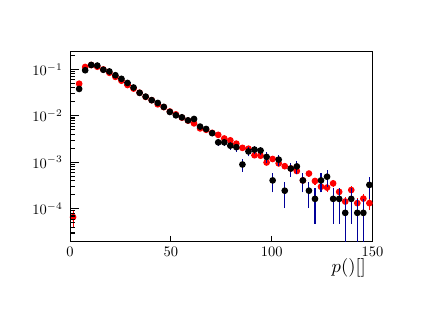
\begin{tikzpicture}
\pgfdeclareplotmark{cross} {
\pgfpathmoveto{\pgfpoint{-0.3\pgfplotmarksize}{\pgfplotmarksize}}
\pgfpathlineto{\pgfpoint{+0.3\pgfplotmarksize}{\pgfplotmarksize}}
\pgfpathlineto{\pgfpoint{+0.3\pgfplotmarksize}{0.3\pgfplotmarksize}}
\pgfpathlineto{\pgfpoint{+1\pgfplotmarksize}{0.3\pgfplotmarksize}}
\pgfpathlineto{\pgfpoint{+1\pgfplotmarksize}{-0.3\pgfplotmarksize}}
\pgfpathlineto{\pgfpoint{+0.3\pgfplotmarksize}{-0.3\pgfplotmarksize}}
\pgfpathlineto{\pgfpoint{+0.3\pgfplotmarksize}{-1.\pgfplotmarksize}}
\pgfpathlineto{\pgfpoint{-0.3\pgfplotmarksize}{-1.\pgfplotmarksize}}
\pgfpathlineto{\pgfpoint{-0.3\pgfplotmarksize}{-0.3\pgfplotmarksize}}
\pgfpathlineto{\pgfpoint{-1.\pgfplotmarksize}{-0.3\pgfplotmarksize}}
\pgfpathlineto{\pgfpoint{-1.\pgfplotmarksize}{0.3\pgfplotmarksize}}
\pgfpathlineto{\pgfpoint{-0.3\pgfplotmarksize}{0.3\pgfplotmarksize}}
\pgfpathclose
\pgfusepathqstroke
}
\pgfdeclareplotmark{cross*} {
\pgfpathmoveto{\pgfpoint{-0.3\pgfplotmarksize}{\pgfplotmarksize}}
\pgfpathlineto{\pgfpoint{+0.3\pgfplotmarksize}{\pgfplotmarksize}}
\pgfpathlineto{\pgfpoint{+0.3\pgfplotmarksize}{0.3\pgfplotmarksize}}
\pgfpathlineto{\pgfpoint{+1\pgfplotmarksize}{0.3\pgfplotmarksize}}
\pgfpathlineto{\pgfpoint{+1\pgfplotmarksize}{-0.3\pgfplotmarksize}}
\pgfpathlineto{\pgfpoint{+0.3\pgfplotmarksize}{-0.3\pgfplotmarksize}}
\pgfpathlineto{\pgfpoint{+0.3\pgfplotmarksize}{-1.\pgfplotmarksize}}
\pgfpathlineto{\pgfpoint{-0.3\pgfplotmarksize}{-1.\pgfplotmarksize}}
\pgfpathlineto{\pgfpoint{-0.3\pgfplotmarksize}{-0.3\pgfplotmarksize}}
\pgfpathlineto{\pgfpoint{-1.\pgfplotmarksize}{-0.3\pgfplotmarksize}}
\pgfpathlineto{\pgfpoint{-1.\pgfplotmarksize}{0.3\pgfplotmarksize}}
\pgfpathlineto{\pgfpoint{-0.3\pgfplotmarksize}{0.3\pgfplotmarksize}}
\pgfpathclose
\pgfusepathqfillstroke
}
\pgfdeclareplotmark{newstar} {
\pgfpathmoveto{\pgfqpoint{0pt}{\pgfplotmarksize}}
\pgfpathlineto{\pgfqpointpolar{44}{0.5\pgfplotmarksize}}
\pgfpathlineto{\pgfqpointpolar{18}{\pgfplotmarksize}}
\pgfpathlineto{\pgfqpointpolar{-20}{0.5\pgfplotmarksize}}
\pgfpathlineto{\pgfqpointpolar{-54}{\pgfplotmarksize}}
\pgfpathlineto{\pgfqpointpolar{-90}{0.5\pgfplotmarksize}}
\pgfpathlineto{\pgfqpointpolar{234}{\pgfplotmarksize}}
\pgfpathlineto{\pgfqpointpolar{198}{0.5\pgfplotmarksize}}
\pgfpathlineto{\pgfqpointpolar{162}{\pgfplotmarksize}}
\pgfpathlineto{\pgfqpointpolar{134}{0.5\pgfplotmarksize}}
\pgfpathclose
\pgfusepathqstroke
}
\pgfdeclareplotmark{newstar*} {
\pgfpathmoveto{\pgfqpoint{0pt}{\pgfplotmarksize}}
\pgfpathlineto{\pgfqpointpolar{44}{0.5\pgfplotmarksize}}
\pgfpathlineto{\pgfqpointpolar{18}{\pgfplotmarksize}}
\pgfpathlineto{\pgfqpointpolar{-20}{0.5\pgfplotmarksize}}
\pgfpathlineto{\pgfqpointpolar{-54}{\pgfplotmarksize}}
\pgfpathlineto{\pgfqpointpolar{-90}{0.5\pgfplotmarksize}}
\pgfpathlineto{\pgfqpointpolar{234}{\pgfplotmarksize}}
\pgfpathlineto{\pgfqpointpolar{198}{0.5\pgfplotmarksize}}
\pgfpathlineto{\pgfqpointpolar{162}{\pgfplotmarksize}}
\pgfpathlineto{\pgfqpointpolar{134}{0.5\pgfplotmarksize}}
\pgfpathclose
\pgfusepathqfillstroke
}
\definecolor{c}{rgb}{1,1,1};
\draw [color=c, fill=c] (5.1,3.20034) rectangle (9.9,6.21242);
\draw [color=c, fill=c] (5.58,3.50154) rectangle (9.42,5.91121);
\definecolor{c}{rgb}{0,0,0};
\draw [c] (5.58,3.50154) -- (5.58,5.91121) -- (9.42,5.91121) -- (9.42,3.50154) -- (5.58,3.50154);
\definecolor{c}{rgb}{1,0,0};
\draw [c] (5.6184,3.67911) -- (5.6184,3.81351);
\draw [c] (5.6184,3.81351) -- (5.6184,3.90121);
\draw [c] (5.58,3.81351) -- (5.6184,3.81351);
\draw [c] (5.6184,3.81351) -- (5.6568,3.81351);
\foreach \P in {(5.6184,3.81351)}{\draw[mark options={color=c,fill=c},mark size=2.402402pt,mark=*,mark size=1pt] plot coordinates {\P};}
\draw [c] (5.6952,5.50389) -- (5.6952,5.50775);
\draw [c] (5.6952,5.50775) -- (5.6952,5.51156);
\draw [c] (5.6568,5.50775) -- (5.6952,5.50775);
\draw [c] (5.6952,5.50775) -- (5.7336,5.50775);
\foreach \P in {(5.6952,5.50775)}{\draw[mark options={color=c,fill=c},mark size=2.402402pt,mark=*,mark size=1pt] plot coordinates {\P};}
\draw [c] (5.772,5.71769) -- (5.772,5.72023);
\draw [c] (5.772,5.72023) -- (5.772,5.72275);
\draw [c] (5.7336,5.72023) -- (5.772,5.72023);
\draw [c] (5.772,5.72023) -- (5.8104,5.72023);
\foreach \P in {(5.772,5.72023)}{\draw[mark options={color=c,fill=c},mark size=2.402402pt,mark=*,mark size=1pt] plot coordinates {\P};}
\draw [c] (5.8488,5.74268) -- (5.8488,5.7451);
\draw [c] (5.8488,5.7451) -- (5.8488,5.7475);
\draw [c] (5.8104,5.7451) -- (5.8488,5.7451);
\draw [c] (5.8488,5.7451) -- (5.8872,5.7451);
\foreach \P in {(5.8488,5.7451)}{\draw[mark options={color=c,fill=c},mark size=2.402402pt,mark=*,mark size=1pt] plot coordinates {\P};}
\draw [c] (5.9256,5.72103) -- (5.9256,5.72356);
\draw [c] (5.9256,5.72356) -- (5.9256,5.72606);
\draw [c] (5.8872,5.72356) -- (5.9256,5.72356);
\draw [c] (5.9256,5.72356) -- (5.964,5.72356);
\foreach \P in {(5.9256,5.72356)}{\draw[mark options={color=c,fill=c},mark size=2.402402pt,mark=*,mark size=1pt] plot coordinates {\P};}
\draw [c] (6.0024,5.68602) -- (6.0024,5.68873);
\draw [c] (6.0024,5.68873) -- (6.0024,5.69141);
\draw [c] (5.964,5.68873) -- (6.0024,5.68873);
\draw [c] (6.0024,5.68873) -- (6.0408,5.68873);
\foreach \P in {(6.0024,5.68873)}{\draw[mark options={color=c,fill=c},mark size=2.402402pt,mark=*,mark size=1pt] plot coordinates {\P};}
\draw [c] (6.0792,5.64398) -- (6.0792,5.64692);
\draw [c] (6.0792,5.64692) -- (6.0792,5.64982);
\draw [c] (6.0408,5.64692) -- (6.0792,5.64692);
\draw [c] (6.0792,5.64692) -- (6.1176,5.64692);
\foreach \P in {(6.0792,5.64692)}{\draw[mark options={color=c,fill=c},mark size=2.402402pt,mark=*,mark size=1pt] plot coordinates {\P};}
\draw [c] (6.156,5.59152) -- (6.156,5.59477);
\draw [c] (6.156,5.59477) -- (6.156,5.59798);
\draw [c] (6.1176,5.59477) -- (6.156,5.59477);
\draw [c] (6.156,5.59477) -- (6.1944,5.59477);
\foreach \P in {(6.156,5.59477)}{\draw[mark options={color=c,fill=c},mark size=2.402402pt,mark=*,mark size=1pt] plot coordinates {\P};}
\draw [c] (6.2328,5.54246) -- (6.2328,5.54604);
\draw [c] (6.2328,5.54604) -- (6.2328,5.54957);
\draw [c] (6.1944,5.54604) -- (6.2328,5.54604);
\draw [c] (6.2328,5.54604) -- (6.2712,5.54604);
\foreach \P in {(6.2328,5.54604)}{\draw[mark options={color=c,fill=c},mark size=2.402402pt,mark=*,mark size=1pt] plot coordinates {\P};}
\draw [c] (6.3096,5.48726) -- (6.3096,5.49125);
\draw [c] (6.3096,5.49125) -- (6.3096,5.49518);
\draw [c] (6.2712,5.49125) -- (6.3096,5.49125);
\draw [c] (6.3096,5.49125) -- (6.348,5.49125);
\foreach \P in {(6.3096,5.49125)}{\draw[mark options={color=c,fill=c},mark size=2.402402pt,mark=*,mark size=1pt] plot coordinates {\P};}
\draw [c] (6.3864,5.44142) -- (6.3864,5.44578);
\draw [c] (6.3864,5.44578) -- (6.3864,5.45006);
\draw [c] (6.348,5.44578) -- (6.3864,5.44578);
\draw [c] (6.3864,5.44578) -- (6.4248,5.44578);
\foreach \P in {(6.3864,5.44578)}{\draw[mark options={color=c,fill=c},mark size=2.402402pt,mark=*,mark size=1pt] plot coordinates {\P};}
\draw [c] (6.4632,5.38859) -- (6.4632,5.39342);
\draw [c] (6.4632,5.39342) -- (6.4632,5.39817);
\draw [c] (6.4248,5.39342) -- (6.4632,5.39342);
\draw [c] (6.4632,5.39342) -- (6.5016,5.39342);
\foreach \P in {(6.4632,5.39342)}{\draw[mark options={color=c,fill=c},mark size=2.402402pt,mark=*,mark size=1pt] plot coordinates {\P};}
\draw [c] (6.54,5.33504) -- (6.54,5.34041);
\draw [c] (6.54,5.34041) -- (6.54,5.34567);
\draw [c] (6.5016,5.34041) -- (6.54,5.34041);
\draw [c] (6.54,5.34041) -- (6.5784,5.34041);
\foreach \P in {(6.54,5.34041)}{\draw[mark options={color=c,fill=c},mark size=2.402402pt,mark=*,mark size=1pt] plot coordinates {\P};}
\draw [c] (6.6168,5.29257) -- (6.6168,5.2984);
\draw [c] (6.6168,5.2984) -- (6.6168,5.3041);
\draw [c] (6.5784,5.2984) -- (6.6168,5.2984);
\draw [c] (6.6168,5.2984) -- (6.6552,5.2984);
\foreach \P in {(6.6168,5.2984)}{\draw[mark options={color=c,fill=c},mark size=2.402402pt,mark=*,mark size=1pt] plot coordinates {\P};}
\draw [c] (6.6936,5.23943) -- (6.6936,5.24589);
\draw [c] (6.6936,5.24589) -- (6.6936,5.2522);
\draw [c] (6.6552,5.24589) -- (6.6936,5.24589);
\draw [c] (6.6936,5.24589) -- (6.732,5.24589);
\foreach \P in {(6.6936,5.24589)}{\draw[mark options={color=c,fill=c},mark size=2.402402pt,mark=*,mark size=1pt] plot coordinates {\P};}
\draw [c] (6.7704,5.20368) -- (6.7704,5.21062);
\draw [c] (6.7704,5.21062) -- (6.7704,5.21737);
\draw [c] (6.732,5.21062) -- (6.7704,5.21062);
\draw [c] (6.7704,5.21062) -- (6.8088,5.21062);
\foreach \P in {(6.7704,5.21062)}{\draw[mark options={color=c,fill=c},mark size=2.402402pt,mark=*,mark size=1pt] plot coordinates {\P};}
\draw [c] (6.8472,5.14694) -- (6.8472,5.15468);
\draw [c] (6.8472,5.15468) -- (6.8472,5.1622);
\draw [c] (6.8088,5.15468) -- (6.8472,5.15468);
\draw [c] (6.8472,5.15468) -- (6.8856,5.15468);
\foreach \P in {(6.8472,5.15468)}{\draw[mark options={color=c,fill=c},mark size=2.402402pt,mark=*,mark size=1pt] plot coordinates {\P};}
\draw [c] (6.924,5.10977) -- (6.924,5.1181);
\draw [c] (6.924,5.1181) -- (6.924,5.12616);
\draw [c] (6.8856,5.1181) -- (6.924,5.1181);
\draw [c] (6.924,5.1181) -- (6.9624,5.1181);
\foreach \P in {(6.924,5.1181)}{\draw[mark options={color=c,fill=c},mark size=2.402402pt,mark=*,mark size=1pt] plot coordinates {\P};}
\draw [c] (7.0008,5.06759) -- (7.0008,5.07663);
\draw [c] (7.0008,5.07663) -- (7.0008,5.08537);
\draw [c] (6.9624,5.07663) -- (7.0008,5.07663);
\draw [c] (7.0008,5.07663) -- (7.0392,5.07663);
\foreach \P in {(7.0008,5.07663)}{\draw[mark options={color=c,fill=c},mark size=2.402402pt,mark=*,mark size=1pt] plot coordinates {\P};}
\draw [c] (7.0776,5.02909) -- (7.0776,5.03884);
\draw [c] (7.0776,5.03884) -- (7.0776,5.04823);
\draw [c] (7.0392,5.03884) -- (7.0776,5.03884);
\draw [c] (7.0776,5.03884) -- (7.116,5.03884);
\foreach \P in {(7.0776,5.03884)}{\draw[mark options={color=c,fill=c},mark size=2.402402pt,mark=*,mark size=1pt] plot coordinates {\P};}
\draw [c] (7.1544,4.99362) -- (7.1544,5.00407);
\draw [c] (7.1544,5.00407) -- (7.1544,5.01411);
\draw [c] (7.116,5.00407) -- (7.1544,5.00407);
\draw [c] (7.1544,5.00407) -- (7.1928,5.00407);
\foreach \P in {(7.1544,5.00407)}{\draw[mark options={color=c,fill=c},mark size=2.402402pt,mark=*,mark size=1pt] plot coordinates {\P};}
\draw [c] (7.2312,4.92841) -- (7.2312,4.94027);
\draw [c] (7.2312,4.94027) -- (7.2312,4.95161);
\draw [c] (7.1928,4.94027) -- (7.2312,4.94027);
\draw [c] (7.2312,4.94027) -- (7.2696,4.94027);
\foreach \P in {(7.2312,4.94027)}{\draw[mark options={color=c,fill=c},mark size=2.402402pt,mark=*,mark size=1pt] plot coordinates {\P};}
\draw [c] (7.308,4.91004) -- (7.308,4.92234);
\draw [c] (7.308,4.92234) -- (7.308,4.93407);
\draw [c] (7.2696,4.92234) -- (7.308,4.92234);
\draw [c] (7.308,4.92234) -- (7.3464,4.92234);
\foreach \P in {(7.308,4.92234)}{\draw[mark options={color=c,fill=c},mark size=2.402402pt,mark=*,mark size=1pt] plot coordinates {\P};}
\draw [c] (7.3848,4.87021) -- (7.3848,4.8835);
\draw [c] (7.3848,4.8835) -- (7.3848,4.89614);
\draw [c] (7.3464,4.8835) -- (7.3848,4.8835);
\draw [c] (7.3848,4.8835) -- (7.4232,4.8835);
\foreach \P in {(7.3848,4.8835)}{\draw[mark options={color=c,fill=c},mark size=2.402402pt,mark=*,mark size=1pt] plot coordinates {\P};}
\draw [c] (7.4616,4.84405) -- (7.4616,4.85804);
\draw [c] (7.4616,4.85804) -- (7.4616,4.8713);
\draw [c] (7.4232,4.85804) -- (7.4616,4.85804);
\draw [c] (7.4616,4.85804) -- (7.5,4.85804);
\foreach \P in {(7.4616,4.85804)}{\draw[mark options={color=c,fill=c},mark size=2.402402pt,mark=*,mark size=1pt] plot coordinates {\P};}
\draw [c] (7.5384,4.79686) -- (7.5384,4.8122);
\draw [c] (7.5384,4.8122) -- (7.5384,4.82667);
\draw [c] (7.5,4.8122) -- (7.5384,4.8122);
\draw [c] (7.5384,4.8122) -- (7.5768,4.8122);
\foreach \P in {(7.5384,4.8122)}{\draw[mark options={color=c,fill=c},mark size=2.402402pt,mark=*,mark size=1pt] plot coordinates {\P};}
\draw [c] (7.6152,4.77256) -- (7.6152,4.78865);
\draw [c] (7.6152,4.78865) -- (7.6152,4.80378);
\draw [c] (7.5768,4.78865) -- (7.6152,4.78865);
\draw [c] (7.6152,4.78865) -- (7.6536,4.78865);
\foreach \P in {(7.6152,4.78865)}{\draw[mark options={color=c,fill=c},mark size=2.402402pt,mark=*,mark size=1pt] plot coordinates {\P};}
\draw [c] (7.692,4.72895) -- (7.692,4.74646);
\draw [c] (7.692,4.74646) -- (7.692,4.76285);
\draw [c] (7.6536,4.74646) -- (7.692,4.74646);
\draw [c] (7.692,4.74646) -- (7.7304,4.74646);
\foreach \P in {(7.692,4.74646)}{\draw[mark options={color=c,fill=c},mark size=2.402402pt,mark=*,mark size=1pt] plot coordinates {\P};}
\draw [c] (7.7688,4.67367) -- (7.7688,4.69318);
\draw [c] (7.7688,4.69318) -- (7.7688,4.71131);
\draw [c] (7.7304,4.69318) -- (7.7688,4.69318);
\draw [c] (7.7688,4.69318) -- (7.8072,4.69318);
\foreach \P in {(7.7688,4.69318)}{\draw[mark options={color=c,fill=c},mark size=2.402402pt,mark=*,mark size=1pt] plot coordinates {\P};}
\draw [c] (7.8456,4.66196) -- (7.8456,4.68192);
\draw [c] (7.8456,4.68192) -- (7.8456,4.70044);
\draw [c] (7.8072,4.68192) -- (7.8456,4.68192);
\draw [c] (7.8456,4.68192) -- (7.884,4.68192);
\foreach \P in {(7.8456,4.68192)}{\draw[mark options={color=c,fill=c},mark size=2.402402pt,mark=*,mark size=1pt] plot coordinates {\P};}
\draw [c] (7.9224,4.57583) -- (7.9224,4.59944);
\draw [c] (7.9224,4.59944) -- (7.9224,4.62106);
\draw [c] (7.884,4.59944) -- (7.9224,4.59944);
\draw [c] (7.9224,4.59944) -- (7.9608,4.59944);
\foreach \P in {(7.9224,4.59944)}{\draw[mark options={color=c,fill=c},mark size=2.402402pt,mark=*,mark size=1pt] plot coordinates {\P};}
\draw [c] (7.9992,4.56951) -- (7.9992,4.59341);
\draw [c] (7.9992,4.59341) -- (7.9992,4.61527);
\draw [c] (7.9608,4.59341) -- (7.9992,4.59341);
\draw [c] (7.9992,4.59341) -- (8.0376,4.59341);
\foreach \P in {(7.9992,4.59341)}{\draw[mark options={color=c,fill=c},mark size=2.402402pt,mark=*,mark size=1pt] plot coordinates {\P};}
\draw [c] (8.076,4.47869) -- (8.076,4.50722);
\draw [c] (8.076,4.50722) -- (8.076,4.53289);
\draw [c] (8.0376,4.50722) -- (8.076,4.50722);
\draw [c] (8.076,4.50722) -- (8.1144,4.50722);
\foreach \P in {(8.076,4.50722)}{\draw[mark options={color=c,fill=c},mark size=2.402402pt,mark=*,mark size=1pt] plot coordinates {\P};}
\draw [c] (8.1528,4.5255) -- (8.1528,4.55154);
\draw [c] (8.1528,4.55154) -- (8.1528,4.57518);
\draw [c] (8.1144,4.55154) -- (8.1528,4.55154);
\draw [c] (8.1528,4.55154) -- (8.1912,4.55154);
\foreach \P in {(8.1528,4.55154)}{\draw[mark options={color=c,fill=c},mark size=2.402402pt,mark=*,mark size=1pt] plot coordinates {\P};}
\draw [c] (8.2296,4.46635) -- (8.2296,4.49557);
\draw [c] (8.2296,4.49557) -- (8.2296,4.52181);
\draw [c] (8.1912,4.49557) -- (8.2296,4.49557);
\draw [c] (8.2296,4.49557) -- (8.268,4.49557);
\foreach \P in {(8.2296,4.49557)}{\draw[mark options={color=c,fill=c},mark size=2.402402pt,mark=*,mark size=1pt] plot coordinates {\P};}
\draw [c] (8.3064,4.42908) -- (8.3064,4.46052);
\draw [c] (8.3064,4.46052) -- (8.3064,4.48851);
\draw [c] (8.268,4.46052) -- (8.3064,4.46052);
\draw [c] (8.3064,4.46052) -- (8.3448,4.46052);
\foreach \P in {(8.3064,4.46052)}{\draw[mark options={color=c,fill=c},mark size=2.402402pt,mark=*,mark size=1pt] plot coordinates {\P};}
\draw [c] (8.3832,4.39824) -- (8.3832,4.43162);
\draw [c] (8.3832,4.43162) -- (8.3832,4.46115);
\draw [c] (8.3448,4.43162) -- (8.3832,4.43162);
\draw [c] (8.3832,4.43162) -- (8.4216,4.43162);
\foreach \P in {(8.3832,4.43162)}{\draw[mark options={color=c,fill=c},mark size=2.402402pt,mark=*,mark size=1pt] plot coordinates {\P};}
\draw [c] (8.46,4.36332) -- (8.46,4.39905);
\draw [c] (8.46,4.39905) -- (8.46,4.4304);
\draw [c] (8.4216,4.39905) -- (8.46,4.39905);
\draw [c] (8.46,4.39905) -- (8.4984,4.39905);
\foreach \P in {(8.46,4.39905)}{\draw[mark options={color=c,fill=c},mark size=2.402402pt,mark=*,mark size=1pt] plot coordinates {\P};}
\draw [c] (8.5368,4.23351) -- (8.5368,4.27952);
\draw [c] (8.5368,4.27952) -- (8.5368,4.31851);
\draw [c] (8.4984,4.27952) -- (8.5368,4.27952);
\draw [c] (8.5368,4.27952) -- (8.5752,4.27952);
\foreach \P in {(8.5368,4.27952)}{\draw[mark options={color=c,fill=c},mark size=2.402402pt,mark=*,mark size=1pt] plot coordinates {\P};}
\draw [c] (8.6136,4.32845) -- (8.6136,4.3667);
\draw [c] (8.6136,4.3667) -- (8.6136,4.39996);
\draw [c] (8.5752,4.3667) -- (8.6136,4.3667);
\draw [c] (8.6136,4.3667) -- (8.652,4.3667);
\foreach \P in {(8.6136,4.3667)}{\draw[mark options={color=c,fill=c},mark size=2.402402pt,mark=*,mark size=1pt] plot coordinates {\P};}
\draw [c] (8.6904,4.22579) -- (8.6904,4.2725);
\draw [c] (8.6904,4.2725) -- (8.6904,4.31199);
\draw [c] (8.652,4.2725) -- (8.6904,4.2725);
\draw [c] (8.6904,4.2725) -- (8.7288,4.2725);
\foreach \P in {(8.6904,4.2725)}{\draw[mark options={color=c,fill=c},mark size=2.402402pt,mark=*,mark size=1pt] plot coordinates {\P};}
\draw [c] (8.7672,4.14405) -- (8.7672,4.1988);
\draw [c] (8.7672,4.1988) -- (8.7672,4.24389);
\draw [c] (8.7288,4.1988) -- (8.7672,4.1988);
\draw [c] (8.7672,4.1988) -- (8.8056,4.1988);
\foreach \P in {(8.7672,4.1988)}{\draw[mark options={color=c,fill=c},mark size=2.402402pt,mark=*,mark size=1pt] plot coordinates {\P};}
\draw [c] (8.844,4.13321) -- (8.844,4.18914);
\draw [c] (8.844,4.18914) -- (8.844,4.23501);
\draw [c] (8.8056,4.18914) -- (8.844,4.18914);
\draw [c] (8.844,4.18914) -- (8.8824,4.18914);
\foreach \P in {(8.844,4.18914)}{\draw[mark options={color=c,fill=c},mark size=2.402402pt,mark=*,mark size=1pt] plot coordinates {\P};}
\draw [c] (8.9208,4.19249) -- (8.9208,4.24233);
\draw [c] (8.9208,4.24233) -- (8.9208,4.28402);
\draw [c] (8.8824,4.24233) -- (8.9208,4.24233);
\draw [c] (8.9208,4.24233) -- (8.9592,4.24233);
\foreach \P in {(8.9208,4.24233)}{\draw[mark options={color=c,fill=c},mark size=2.402402pt,mark=*,mark size=1pt] plot coordinates {\P};}
\draw [c] (8.9976,4.07136) -- (8.9976,4.13442);
\draw [c] (8.9976,4.13442) -- (8.9976,4.18499);
\draw [c] (8.9592,4.13442) -- (8.9976,4.13442);
\draw [c] (8.9976,4.13442) -- (9.036,4.13442);
\foreach \P in {(8.9976,4.13442)}{\draw[mark options={color=c,fill=c},mark size=2.402402pt,mark=*,mark size=1pt] plot coordinates {\P};}
\draw [c] (9.0744,3.92836) -- (9.0744,4.01157);
\draw [c] (9.0744,4.01157) -- (9.0744,4.07428);
\draw [c] (9.036,4.01157) -- (9.0744,4.01157);
\draw [c] (9.0744,4.01157) -- (9.1128,4.01157);
\foreach \P in {(9.0744,4.01157)}{\draw[mark options={color=c,fill=c},mark size=2.402402pt,mark=*,mark size=1pt] plot coordinates {\P};}
\draw [c] (9.1512,4.09783) -- (9.1512,4.15773);
\draw [c] (9.1512,4.15773) -- (9.1512,4.20624);
\draw [c] (9.1128,4.15773) -- (9.1512,4.15773);
\draw [c] (9.1512,4.15773) -- (9.1896,4.15773);
\foreach \P in {(9.1512,4.15773)}{\draw[mark options={color=c,fill=c},mark size=2.402402pt,mark=*,mark size=1pt] plot coordinates {\P};}
\draw [c] (9.228,3.90381) -- (9.228,3.99107);
\draw [c] (9.228,3.99107) -- (9.228,4.05604);
\draw [c] (9.1896,3.99107) -- (9.228,3.99107);
\draw [c] (9.228,3.99107) -- (9.2664,3.99107);
\foreach \P in {(9.228,3.99107)}{\draw[mark options={color=c,fill=c},mark size=2.402402pt,mark=*,mark size=1pt] plot coordinates {\P};}
\draw [c] (9.3048,3.97172) -- (9.3048,4.04823);
\draw [c] (9.3048,4.04823) -- (9.3048,4.10707);
\draw [c] (9.2664,4.04823) -- (9.3048,4.04823);
\draw [c] (9.3048,4.04823) -- (9.3432,4.04823);
\foreach \P in {(9.3048,4.04823)}{\draw[mark options={color=c,fill=c},mark size=2.402402pt,mark=*,mark size=1pt] plot coordinates {\P};}
\draw [c] (9.3816,3.90381) -- (9.3816,3.99107);
\draw [c] (9.3816,3.99107) -- (9.3816,4.05604);
\draw [c] (9.3432,3.99107) -- (9.3816,3.99107);
\draw [c] (9.3816,3.99107) -- (9.42,3.99107);
\foreach \P in {(9.3816,3.99107)}{\draw[mark options={color=c,fill=c},mark size=2.402402pt,mark=*,mark size=1pt] plot coordinates {\P};}
\definecolor{c}{rgb}{0,0,0};
\draw [c] (5.58,3.50154) -- (9.42,3.50154);
\draw [anchor= east] (9.42,3.16419) node[scale=0.672711, rotate=0]{$p(\pion) [\mevc]$};
\draw [c] (5.58,3.57383) -- (5.58,3.50154);
\draw [c] (6.86,3.57383) -- (6.86,3.50154);
\draw [c] (8.14,3.57383) -- (8.14,3.50154);
\draw [c] (9.42,3.57383) -- (9.42,3.50154);
\draw [anchor=base] (5.58,3.30877) node[scale=0.52322, rotate=0]{0};
\draw [anchor=base] (6.86,3.30877) node[scale=0.52322, rotate=0]{50};
\draw [anchor=base] (8.14,3.30877) node[scale=0.52322, rotate=0]{100};
\draw [anchor=base] (9.42,3.30877) node[scale=0.52322, rotate=0]{150};
\draw [c] (5.58,3.50154) -- (5.58,5.91121);
\draw [c] (5.6376,3.50734) -- (5.58,3.50734);
\draw [c] (5.6376,3.61121) -- (5.58,3.61121);
\draw [c] (5.6376,3.6849) -- (5.58,3.6849);
\draw [c] (5.6376,3.74207) -- (5.58,3.74207);
\draw [c] (5.6376,3.78877) -- (5.58,3.78877);
\draw [c] (5.6376,3.82826) -- (5.58,3.82826);
\draw [c] (5.6376,3.86247) -- (5.58,3.86247);
\draw [c] (5.6376,3.89264) -- (5.58,3.89264);
\draw [c] (5.6952,3.91963) -- (5.58,3.91963);
\draw [anchor= east] (5.54928,3.91963) node[scale=0.52322, rotate=0]{$10^{-4}$};
\draw [c] (5.6376,4.09719) -- (5.58,4.09719);
\draw [c] (5.6376,4.20106) -- (5.58,4.20106);
\draw [c] (5.6376,4.27475) -- (5.58,4.27475);
\draw [c] (5.6376,4.33191) -- (5.58,4.33191);
\draw [c] (5.6376,4.37862) -- (5.58,4.37862);
\draw [c] (5.6376,4.41811) -- (5.58,4.41811);
\draw [c] (5.6376,4.45231) -- (5.58,4.45231);
\draw [c] (5.6376,4.48248) -- (5.58,4.48248);
\draw [c] (5.6952,4.50947) -- (5.58,4.50947);
\draw [anchor= east] (5.54928,4.50947) node[scale=0.52322, rotate=0]{$10^{-3}$};
\draw [c] (5.6376,4.68704) -- (5.58,4.68704);
\draw [c] (5.6376,4.7909) -- (5.58,4.7909);
\draw [c] (5.6376,4.8646) -- (5.58,4.8646);
\draw [c] (5.6376,4.92176) -- (5.58,4.92176);
\draw [c] (5.6376,4.96846) -- (5.58,4.96846);
\draw [c] (5.6376,5.00795) -- (5.58,5.00795);
\draw [c] (5.6376,5.04216) -- (5.58,5.04216);
\draw [c] (5.6376,5.07233) -- (5.58,5.07233);
\draw [c] (5.6952,5.09932) -- (5.58,5.09932);
\draw [anchor= east] (5.54928,5.09932) node[scale=0.52322, rotate=0]{$10^{-2}$};
\draw [c] (5.6376,5.27688) -- (5.58,5.27688);
\draw [c] (5.6376,5.38075) -- (5.58,5.38075);
\draw [c] (5.6376,5.45444) -- (5.58,5.45444);
\draw [c] (5.6376,5.5116) -- (5.58,5.5116);
\draw [c] (5.6376,5.55831) -- (5.58,5.55831);
\draw [c] (5.6376,5.5978) -- (5.58,5.5978);
\draw [c] (5.6376,5.632) -- (5.58,5.632);
\draw [c] (5.6376,5.66218) -- (5.58,5.66218);
\draw [c] (5.6952,5.68917) -- (5.58,5.68917);
\draw [anchor= east] (5.54928,5.68917) node[scale=0.52322, rotate=0]{$10^{-1}$};
\draw [c] (5.6376,5.86673) -- (5.58,5.86673);
\definecolor{c}{rgb}{0,0,0.6};
\draw [c] (5.6952,5.4293) -- (5.6952,5.44145);
\draw [c] (5.6952,5.44145) -- (5.6952,5.45305);
\draw [c] (5.6568,5.44145) -- (5.6952,5.44145);
\draw [c] (5.6952,5.44145) -- (5.7336,5.44145);
\definecolor{c}{rgb}{0,0,0};
\foreach \P in {(5.6952,5.44145)}{\draw[mark options={color=c,fill=c},mark size=2.402402pt,mark=*,mark size=1pt] plot coordinates {\P};}
\definecolor{c}{rgb}{0,0,0.6};
\draw [c] (5.772,5.671) -- (5.772,5.67858);
\draw [c] (5.772,5.67858) -- (5.772,5.68595);
\draw [c] (5.7336,5.67858) -- (5.772,5.67858);
\draw [c] (5.772,5.67858) -- (5.8104,5.67858);
\definecolor{c}{rgb}{0,0,0};
\foreach \P in {(5.772,5.67858)}{\draw[mark options={color=c,fill=c},mark size=2.402402pt,mark=*,mark size=1pt] plot coordinates {\P};}
\definecolor{c}{rgb}{0,0,0.6};
\draw [c] (5.8488,5.73902) -- (5.8488,5.74566);
\draw [c] (5.8488,5.74566) -- (5.8488,5.75213);
\draw [c] (5.8104,5.74566) -- (5.8488,5.74566);
\draw [c] (5.8488,5.74566) -- (5.8872,5.74566);
\definecolor{c}{rgb}{0,0,0};
\foreach \P in {(5.8488,5.74566)}{\draw[mark options={color=c,fill=c},mark size=2.402402pt,mark=*,mark size=1pt] plot coordinates {\P};}
\definecolor{c}{rgb}{0,0,0.6};
\draw [c] (5.9256,5.73109) -- (5.9256,5.73783);
\draw [c] (5.9256,5.73783) -- (5.9256,5.7444);
\draw [c] (5.8872,5.73783) -- (5.9256,5.73783);
\draw [c] (5.9256,5.73783) -- (5.964,5.73783);
\definecolor{c}{rgb}{0,0,0};
\foreach \P in {(5.9256,5.73783)}{\draw[mark options={color=c,fill=c},mark size=2.402402pt,mark=*,mark size=1pt] plot coordinates {\P};}
\definecolor{c}{rgb}{0,0,0.6};
\draw [c] (6.0024,5.67755) -- (6.0024,5.68504);
\draw [c] (6.0024,5.68504) -- (6.0024,5.69231);
\draw [c] (5.964,5.68504) -- (6.0024,5.68504);
\draw [c] (6.0024,5.68504) -- (6.0408,5.68504);
\definecolor{c}{rgb}{0,0,0};
\foreach \P in {(6.0024,5.68504)}{\draw[mark options={color=c,fill=c},mark size=2.402402pt,mark=*,mark size=1pt] plot coordinates {\P};}
\definecolor{c}{rgb}{0,0,0.6};
\draw [c] (6.0792,5.65551) -- (6.0792,5.66333);
\draw [c] (6.0792,5.66333) -- (6.0792,5.67091);
\draw [c] (6.0408,5.66333) -- (6.0792,5.66333);
\draw [c] (6.0792,5.66333) -- (6.1176,5.66333);
\definecolor{c}{rgb}{0,0,0};
\foreach \P in {(6.0792,5.66333)}{\draw[mark options={color=c,fill=c},mark size=2.402402pt,mark=*,mark size=1pt] plot coordinates {\P};}
\definecolor{c}{rgb}{0,0,0.6};
\draw [c] (6.156,5.60682) -- (6.156,5.61542);
\draw [c] (6.156,5.61542) -- (6.156,5.62373);
\draw [c] (6.1176,5.61542) -- (6.156,5.61542);
\draw [c] (6.156,5.61542) -- (6.1944,5.61542);
\definecolor{c}{rgb}{0,0,0};
\foreach \P in {(6.156,5.61542)}{\draw[mark options={color=c,fill=c},mark size=2.402402pt,mark=*,mark size=1pt] plot coordinates {\P};}
\definecolor{c}{rgb}{0,0,0.6};
\draw [c] (6.2328,5.56002) -- (6.2328,5.56943);
\draw [c] (6.2328,5.56943) -- (6.2328,5.57852);
\draw [c] (6.1944,5.56943) -- (6.2328,5.56943);
\draw [c] (6.2328,5.56943) -- (6.2712,5.56943);
\definecolor{c}{rgb}{0,0,0};
\foreach \P in {(6.2328,5.56943)}{\draw[mark options={color=c,fill=c},mark size=2.402402pt,mark=*,mark size=1pt] plot coordinates {\P};}
\definecolor{c}{rgb}{0,0,0.6};
\draw [c] (6.3096,5.50703) -- (6.3096,5.51747);
\draw [c] (6.3096,5.51747) -- (6.3096,5.5275);
\draw [c] (6.2712,5.51747) -- (6.3096,5.51747);
\draw [c] (6.3096,5.51747) -- (6.348,5.51747);
\definecolor{c}{rgb}{0,0,0};
\foreach \P in {(6.3096,5.51747)}{\draw[mark options={color=c,fill=c},mark size=2.402402pt,mark=*,mark size=1pt] plot coordinates {\P};}
\definecolor{c}{rgb}{0,0,0.6};
\draw [c] (6.3864,5.44777) -- (6.3864,5.45949);
\draw [c] (6.3864,5.45949) -- (6.3864,5.4707);
\draw [c] (6.348,5.45949) -- (6.3864,5.45949);
\draw [c] (6.3864,5.45949) -- (6.4248,5.45949);
\definecolor{c}{rgb}{0,0,0};
\foreach \P in {(6.3864,5.45949)}{\draw[mark options={color=c,fill=c},mark size=2.402402pt,mark=*,mark size=1pt] plot coordinates {\P};}
\definecolor{c}{rgb}{0,0,0.6};
\draw [c] (6.4632,5.37846) -- (6.4632,5.39187);
\draw [c] (6.4632,5.39187) -- (6.4632,5.40462);
\draw [c] (6.4248,5.39187) -- (6.4632,5.39187);
\draw [c] (6.4632,5.39187) -- (6.5016,5.39187);
\definecolor{c}{rgb}{0,0,0};
\foreach \P in {(6.4632,5.39187)}{\draw[mark options={color=c,fill=c},mark size=2.402402pt,mark=*,mark size=1pt] plot coordinates {\P};}
\definecolor{c}{rgb}{0,0,0.6};
\draw [c] (6.54,5.32878) -- (6.54,5.34356);
\draw [c] (6.54,5.34356) -- (6.54,5.35754);
\draw [c] (6.5016,5.34356) -- (6.54,5.34356);
\draw [c] (6.54,5.34356) -- (6.5784,5.34356);
\definecolor{c}{rgb}{0,0,0};
\foreach \P in {(6.54,5.34356)}{\draw[mark options={color=c,fill=c},mark size=2.402402pt,mark=*,mark size=1pt] plot coordinates {\P};}
\definecolor{c}{rgb}{0,0,0.6};
\draw [c] (6.6168,5.28261) -- (6.6168,5.29878);
\draw [c] (6.6168,5.29878) -- (6.6168,5.314);
\draw [c] (6.5784,5.29878) -- (6.6168,5.29878);
\draw [c] (6.6168,5.29878) -- (6.6552,5.29878);
\definecolor{c}{rgb}{0,0,0};
\foreach \P in {(6.6168,5.29878)}{\draw[mark options={color=c,fill=c},mark size=2.402402pt,mark=*,mark size=1pt] plot coordinates {\P};}
\definecolor{c}{rgb}{0,0,0.6};
\draw [c] (6.6936,5.24653) -- (6.6936,5.26389);
\draw [c] (6.6936,5.26389) -- (6.6936,5.28015);
\draw [c] (6.6552,5.26389) -- (6.6936,5.26389);
\draw [c] (6.6936,5.26389) -- (6.732,5.26389);
\definecolor{c}{rgb}{0,0,0};
\foreach \P in {(6.6936,5.26389)}{\draw[mark options={color=c,fill=c},mark size=2.402402pt,mark=*,mark size=1pt] plot coordinates {\P};}
\definecolor{c}{rgb}{0,0,0.6};
\draw [c] (6.7704,5.19373) -- (6.7704,5.21297);
\draw [c] (6.7704,5.21297) -- (6.7704,5.23087);
\draw [c] (6.732,5.21297) -- (6.7704,5.21297);
\draw [c] (6.7704,5.21297) -- (6.8088,5.21297);
\definecolor{c}{rgb}{0,0,0};
\foreach \P in {(6.7704,5.21297)}{\draw[mark options={color=c,fill=c},mark size=2.402402pt,mark=*,mark size=1pt] plot coordinates {\P};}
\definecolor{c}{rgb}{0,0,0.6};
\draw [c] (6.8472,5.12747) -- (6.8472,5.14936);
\draw [c] (6.8472,5.14936) -- (6.8472,5.16953);
\draw [c] (6.8088,5.14936) -- (6.8472,5.14936);
\draw [c] (6.8472,5.14936) -- (6.8856,5.14936);
\definecolor{c}{rgb}{0,0,0};
\foreach \P in {(6.8472,5.14936)}{\draw[mark options={color=c,fill=c},mark size=2.402402pt,mark=*,mark size=1pt] plot coordinates {\P};}
\definecolor{c}{rgb}{0,0,0.6};
\draw [c] (6.924,5.08251) -- (6.924,5.10641);
\draw [c] (6.924,5.10641) -- (6.924,5.12827);
\draw [c] (6.8856,5.10641) -- (6.924,5.10641);
\draw [c] (6.924,5.10641) -- (6.9624,5.10641);
\definecolor{c}{rgb}{0,0,0};
\foreach \P in {(6.924,5.10641)}{\draw[mark options={color=c,fill=c},mark size=2.402402pt,mark=*,mark size=1pt] plot coordinates {\P};}
\definecolor{c}{rgb}{0,0,0.6};
\draw [c] (7.0008,5.05558) -- (7.0008,5.08077);
\draw [c] (7.0008,5.08077) -- (7.0008,5.10371);
\draw [c] (6.9624,5.08077) -- (7.0008,5.08077);
\draw [c] (7.0008,5.08077) -- (7.0392,5.08077);
\definecolor{c}{rgb}{0,0,0};
\foreach \P in {(7.0008,5.08077)}{\draw[mark options={color=c,fill=c},mark size=2.402402pt,mark=*,mark size=1pt] plot coordinates {\P};}
\definecolor{c}{rgb}{0,0,0.6};
\draw [c] (7.0776,5.01475) -- (7.0776,5.04203);
\draw [c] (7.0776,5.04203) -- (7.0776,5.06668);
\draw [c] (7.0392,5.04203) -- (7.0776,5.04203);
\draw [c] (7.0776,5.04203) -- (7.116,5.04203);
\definecolor{c}{rgb}{0,0,0};
\foreach \P in {(7.0776,5.04203)}{\draw[mark options={color=c,fill=c},mark size=2.402402pt,mark=*,mark size=1pt] plot coordinates {\P};}
\definecolor{c}{rgb}{0,0,0.6};
\draw [c] (7.1544,5.0334) -- (7.1544,5.05971);
\draw [c] (7.1544,5.05971) -- (7.1544,5.08356);
\draw [c] (7.116,5.05971) -- (7.1544,5.05971);
\draw [c] (7.1544,5.05971) -- (7.1928,5.05971);
\definecolor{c}{rgb}{0,0,0};
\foreach \P in {(7.1544,5.05971)}{\draw[mark options={color=c,fill=c},mark size=2.402402pt,mark=*,mark size=1pt] plot coordinates {\P};}
\definecolor{c}{rgb}{0,0,0.6};
\draw [c] (7.2312,4.93093) -- (7.2312,4.96306);
\draw [c] (7.2312,4.96306) -- (7.2312,4.99159);
\draw [c] (7.1928,4.96306) -- (7.2312,4.96306);
\draw [c] (7.2312,4.96306) -- (7.2696,4.96306);
\definecolor{c}{rgb}{0,0,0};
\foreach \P in {(7.2312,4.96306)}{\draw[mark options={color=c,fill=c},mark size=2.402402pt,mark=*,mark size=1pt] plot coordinates {\P};}
\definecolor{c}{rgb}{0,0,0.6};
\draw [c] (7.308,4.89868) -- (7.308,4.93288);
\draw [c] (7.308,4.93288) -- (7.308,4.96306);
\draw [c] (7.2696,4.93288) -- (7.308,4.93288);
\draw [c] (7.308,4.93288) -- (7.3464,4.93288);
\definecolor{c}{rgb}{0,0,0};
\foreach \P in {(7.308,4.93288)}{\draw[mark options={color=c,fill=c},mark size=2.402402pt,mark=*,mark size=1pt] plot coordinates {\P};}
\definecolor{c}{rgb}{0,0,0.6};
\draw [c] (7.3848,4.84145) -- (7.3848,4.87969);
\draw [c] (7.3848,4.87969) -- (7.3848,4.91296);
\draw [c] (7.3464,4.87969) -- (7.3848,4.87969);
\draw [c] (7.3848,4.87969) -- (7.4232,4.87969);
\definecolor{c}{rgb}{0,0,0};
\foreach \P in {(7.3848,4.87969)}{\draw[mark options={color=c,fill=c},mark size=2.402402pt,mark=*,mark size=1pt] plot coordinates {\P};}
\definecolor{c}{rgb}{0,0,0.6};
\draw [c] (7.4616,4.71421) -- (7.4616,4.76321);
\draw [c] (7.4616,4.76321) -- (7.4616,4.80432);
\draw [c] (7.4232,4.76321) -- (7.4616,4.76321);
\draw [c] (7.4616,4.76321) -- (7.5,4.76321);
\definecolor{c}{rgb}{0,0,0};
\foreach \P in {(7.4616,4.76321)}{\draw[mark options={color=c,fill=c},mark size=2.402402pt,mark=*,mark size=1pt] plot coordinates {\P};}
\definecolor{c}{rgb}{0,0,0.6};
\draw [c] (7.5384,4.71421) -- (7.5384,4.76321);
\draw [c] (7.5384,4.76321) -- (7.5384,4.80432);
\draw [c] (7.5,4.76321) -- (7.5384,4.76321);
\draw [c] (7.5384,4.76321) -- (7.5768,4.76321);
\definecolor{c}{rgb}{0,0,0};
\foreach \P in {(7.5384,4.76321)}{\draw[mark options={color=c,fill=c},mark size=2.402402pt,mark=*,mark size=1pt] plot coordinates {\P};}
\definecolor{c}{rgb}{0,0,0.6};
\draw [c] (7.6152,4.66746) -- (7.6152,4.72112);
\draw [c] (7.6152,4.72112) -- (7.6152,4.76546);
\draw [c] (7.5768,4.72112) -- (7.6152,4.72112);
\draw [c] (7.6152,4.72112) -- (7.6536,4.72112);
\definecolor{c}{rgb}{0,0,0};
\foreach \P in {(7.6152,4.72112)}{\draw[mark options={color=c,fill=c},mark size=2.402402pt,mark=*,mark size=1pt] plot coordinates {\P};}
\definecolor{c}{rgb}{0,0,0.6};
\draw [c] (7.692,4.64621) -- (7.692,4.70213);
\draw [c] (7.692,4.70213) -- (7.692,4.74801);
\draw [c] (7.6536,4.70213) -- (7.692,4.70213);
\draw [c] (7.692,4.70213) -- (7.7304,4.70213);
\definecolor{c}{rgb}{0,0,0};
\foreach \P in {(7.692,4.70213)}{\draw[mark options={color=c,fill=c},mark size=2.402402pt,mark=*,mark size=1pt] plot coordinates {\P};}
\definecolor{c}{rgb}{0,0,0.6};
\draw [c] (7.7688,4.38985) -- (7.7688,4.48178);
\draw [c] (7.7688,4.48178) -- (7.7688,4.54928);
\draw [c] (7.7304,4.48178) -- (7.7688,4.48178);
\draw [c] (7.7688,4.48178) -- (7.8072,4.48178);
\definecolor{c}{rgb}{0,0,0};
\foreach \P in {(7.7688,4.48178)}{\draw[mark options={color=c,fill=c},mark size=2.402402pt,mark=*,mark size=1pt] plot coordinates {\P};}
\definecolor{c}{rgb}{0,0,0.6};
\draw [c] (7.8456,4.58436) -- (7.8456,4.64742);
\draw [c] (7.8456,4.64742) -- (7.8456,4.69799);
\draw [c] (7.8072,4.64742) -- (7.8456,4.64742);
\draw [c] (7.8456,4.64742) -- (7.884,4.64742);
\definecolor{c}{rgb}{0,0,0};
\foreach \P in {(7.8456,4.64742)}{\draw[mark options={color=c,fill=c},mark size=2.402402pt,mark=*,mark size=1pt] plot coordinates {\P};}
\definecolor{c}{rgb}{0,0,0.6};
\draw [c] (7.9224,4.61082) -- (7.9224,4.67073);
\draw [c] (7.9224,4.67073) -- (7.9224,4.71924);
\draw [c] (7.884,4.67073) -- (7.9224,4.67073);
\draw [c] (7.9224,4.67073) -- (7.9608,4.67073);
\definecolor{c}{rgb}{0,0,0};
\foreach \P in {(7.9224,4.67073)}{\draw[mark options={color=c,fill=c},mark size=2.402402pt,mark=*,mark size=1pt] plot coordinates {\P};}
\definecolor{c}{rgb}{0,0,0.6};
\draw [c] (7.9992,4.59791) -- (7.9992,4.65934);
\draw [c] (7.9992,4.65934) -- (7.9992,4.70885);
\draw [c] (7.9608,4.65934) -- (7.9992,4.65934);
\draw [c] (7.9992,4.65934) -- (8.0376,4.65934);
\definecolor{c}{rgb}{0,0,0};
\foreach \P in {(7.9992,4.65934)}{\draw[mark options={color=c,fill=c},mark size=2.402402pt,mark=*,mark size=1pt] plot coordinates {\P};}
\definecolor{c}{rgb}{0,0,0.6};
\draw [c] (8.076,4.50407) -- (8.076,4.57776);
\draw [c] (8.076,4.57776) -- (8.076,4.63492);
\draw [c] (8.0376,4.57776) -- (8.076,4.57776);
\draw [c] (8.076,4.57776) -- (8.1144,4.57776);
\definecolor{c}{rgb}{0,0,0};
\foreach \P in {(8.076,4.57776)}{\draw[mark options={color=c,fill=c},mark size=2.402402pt,mark=*,mark size=1pt] plot coordinates {\P};}
\definecolor{c}{rgb}{0,0,0.6};
\draw [c] (8.1528,4.12795) -- (8.1528,4.2798);
\draw [c] (8.1528,4.2798) -- (8.1528,4.37449);
\draw [c] (8.1144,4.2798) -- (8.1528,4.2798);
\draw [c] (8.1528,4.2798) -- (8.1912,4.2798);
\definecolor{c}{rgb}{0,0,0};
\foreach \P in {(8.1528,4.2798)}{\draw[mark options={color=c,fill=c},mark size=2.402402pt,mark=*,mark size=1pt] plot coordinates {\P};}
\definecolor{c}{rgb}{0,0,0.6};
\draw [c] (8.2296,4.4639) -- (8.2296,4.54355);
\draw [c] (8.2296,4.54355) -- (8.2296,4.60423);
\draw [c] (8.1912,4.54355) -- (8.2296,4.54355);
\draw [c] (8.2296,4.54355) -- (8.268,4.54355);
\definecolor{c}{rgb}{0,0,0};
\foreach \P in {(8.2296,4.54355)}{\draw[mark options={color=c,fill=c},mark size=2.402402pt,mark=*,mark size=1pt] plot coordinates {\P};}
\definecolor{c}{rgb}{0,0,0.6};
\draw [c] (8.3064,3.92833) -- (8.3064,4.14894);
\draw [c] (8.3064,4.14894) -- (8.3064,4.26569);
\draw [c] (8.268,4.14894) -- (8.3064,4.14894);
\draw [c] (8.3064,4.14894) -- (8.3448,4.14894);
\definecolor{c}{rgb}{0,0,0};
\foreach \P in {(8.3064,4.14894)}{\draw[mark options={color=c,fill=c},mark size=2.402402pt,mark=*,mark size=1pt] plot coordinates {\P};}
\definecolor{c}{rgb}{0,0,0.6};
\draw [c] (8.3832,4.3265) -- (8.3832,4.43037);
\draw [c] (8.3832,4.43037) -- (8.3832,4.50407);
\draw [c] (8.3448,4.43037) -- (8.3832,4.43037);
\draw [c] (8.3832,4.43037) -- (8.4216,4.43037);
\definecolor{c}{rgb}{0,0,0};
\foreach \P in {(8.3832,4.43037)}{\draw[mark options={color=c,fill=c},mark size=2.402402pt,mark=*,mark size=1pt] plot coordinates {\P};}
\definecolor{c}{rgb}{0,0,0.6};
\draw [c] (8.46,4.35998) -- (8.46,4.45736);
\draw [c] (8.46,4.45736) -- (8.46,4.52775);
\draw [c] (8.4216,4.45736) -- (8.46,4.45736);
\draw [c] (8.46,4.45736) -- (8.4984,4.45736);
\definecolor{c}{rgb}{0,0,0};
\foreach \P in {(8.46,4.45736)}{\draw[mark options={color=c,fill=c},mark size=2.402402pt,mark=*,mark size=1pt] plot coordinates {\P};}
\definecolor{c}{rgb}{0,0,0.6};
\draw [c] (8.5368,4.12795) -- (8.5368,4.2798);
\draw [c] (8.5368,4.2798) -- (8.5368,4.37449);
\draw [c] (8.4984,4.2798) -- (8.5368,4.2798);
\draw [c] (8.5368,4.2798) -- (8.5752,4.2798);
\definecolor{c}{rgb}{0,0,0};
\foreach \P in {(8.5368,4.2798)}{\draw[mark options={color=c,fill=c},mark size=2.402402pt,mark=*,mark size=1pt] plot coordinates {\P};}
\definecolor{c}{rgb}{0,0,0.6};
\draw [c] (8.6136,3.92833) -- (8.6136,4.14894);
\draw [c] (8.6136,4.14894) -- (8.6136,4.26569);
\draw [c] (8.5752,4.14894) -- (8.6136,4.14894);
\draw [c] (8.6136,4.14894) -- (8.652,4.14894);
\definecolor{c}{rgb}{0,0,0};
\foreach \P in {(8.6136,4.14894)}{\draw[mark options={color=c,fill=c},mark size=2.402402pt,mark=*,mark size=1pt] plot coordinates {\P};}
\definecolor{c}{rgb}{0,0,0.6};
\draw [c] (8.6904,3.73052) -- (8.6904,4.04508);
\draw [c] (8.6904,4.04508) -- (8.6904,4.18207);
\draw [c] (8.652,4.04508) -- (8.6904,4.04508);
\draw [c] (8.6904,4.04508) -- (8.7288,4.04508);
\definecolor{c}{rgb}{0,0,0};
\foreach \P in {(8.6904,4.04508)}{\draw[mark options={color=c,fill=c},mark size=2.402402pt,mark=*,mark size=1pt] plot coordinates {\P};}
\definecolor{c}{rgb}{0,0,0.6};
\draw [c] (8.7672,4.12795) -- (8.7672,4.2798);
\draw [c] (8.7672,4.2798) -- (8.7672,4.37449);
\draw [c] (8.7288,4.2798) -- (8.7672,4.2798);
\draw [c] (8.7672,4.2798) -- (8.8056,4.2798);
\definecolor{c}{rgb}{0,0,0};
\foreach \P in {(8.7672,4.2798)}{\draw[mark options={color=c,fill=c},mark size=2.402402pt,mark=*,mark size=1pt] plot coordinates {\P};}
\definecolor{c}{rgb}{0,0,0.6};
\draw [c] (8.844,4.1921) -- (8.844,4.3265);
\draw [c] (8.844,4.3265) -- (8.844,4.4142);
\draw [c] (8.8056,4.3265) -- (8.844,4.3265);
\draw [c] (8.844,4.3265) -- (8.8824,4.3265);
\definecolor{c}{rgb}{0,0,0};
\foreach \P in {(8.844,4.3265)}{\draw[mark options={color=c,fill=c},mark size=2.402402pt,mark=*,mark size=1pt] plot coordinates {\P};}
\definecolor{c}{rgb}{0,0,0.6};
\draw [c] (8.9208,3.73052) -- (8.9208,4.04508);
\draw [c] (8.9208,4.04508) -- (8.9208,4.18207);
\draw [c] (8.8824,4.04508) -- (8.9208,4.04508);
\draw [c] (8.9208,4.04508) -- (8.9592,4.04508);
\definecolor{c}{rgb}{0,0,0};
\foreach \P in {(8.9208,4.04508)}{\draw[mark options={color=c,fill=c},mark size=2.402402pt,mark=*,mark size=1pt] plot coordinates {\P};}
\definecolor{c}{rgb}{0,0,0.6};
\draw [c] (8.9976,3.73052) -- (8.9976,4.04508);
\draw [c] (8.9976,4.04508) -- (8.9976,4.18207);
\draw [c] (8.9592,4.04508) -- (8.9976,4.04508);
\draw [c] (8.9976,4.04508) -- (9.036,4.04508);
\definecolor{c}{rgb}{0,0,0};
\foreach \P in {(8.9976,4.04508)}{\draw[mark options={color=c,fill=c},mark size=2.402402pt,mark=*,mark size=1pt] plot coordinates {\P};}
\definecolor{c}{rgb}{0,0,0.6};
\draw [c] (9.0744,3.50154) -- (9.0744,3.86752);
\draw [c] (9.0744,3.86752) -- (9.0744,4.04508);
\draw [c] (9.036,3.86752) -- (9.0744,3.86752);
\draw [c] (9.0744,3.86752) -- (9.1128,3.86752);
\definecolor{c}{rgb}{0,0,0};
\foreach \P in {(9.0744,3.86752)}{\draw[mark options={color=c,fill=c},mark size=2.402402pt,mark=*,mark size=1pt] plot coordinates {\P};}
\definecolor{c}{rgb}{0,0,0.6};
\draw [c] (9.1512,3.73052) -- (9.1512,4.04508);
\draw [c] (9.1512,4.04508) -- (9.1512,4.18207);
\draw [c] (9.1128,4.04508) -- (9.1512,4.04508);
\draw [c] (9.1512,4.04508) -- (9.1896,4.04508);
\definecolor{c}{rgb}{0,0,0};
\foreach \P in {(9.1512,4.04508)}{\draw[mark options={color=c,fill=c},mark size=2.402402pt,mark=*,mark size=1pt] plot coordinates {\P};}
\definecolor{c}{rgb}{0,0,0.6};
\draw [c] (9.228,3.50154) -- (9.228,3.86752);
\draw [c] (9.228,3.86752) -- (9.228,4.04508);
\draw [c] (9.1896,3.86752) -- (9.228,3.86752);
\draw [c] (9.228,3.86752) -- (9.2664,3.86752);
\definecolor{c}{rgb}{0,0,0};
\foreach \P in {(9.228,3.86752)}{\draw[mark options={color=c,fill=c},mark size=2.402402pt,mark=*,mark size=1pt] plot coordinates {\P};}
\definecolor{c}{rgb}{0,0,0.6};
\draw [c] (9.3048,3.50154) -- (9.3048,3.86752);
\draw [c] (9.3048,3.86752) -- (9.3048,4.04508);
\draw [c] (9.2664,3.86752) -- (9.3048,3.86752);
\draw [c] (9.3048,3.86752) -- (9.3432,3.86752);
\definecolor{c}{rgb}{0,0,0};
\foreach \P in {(9.3048,3.86752)}{\draw[mark options={color=c,fill=c},mark size=2.402402pt,mark=*,mark size=1pt] plot coordinates {\P};}
\definecolor{c}{rgb}{0,0,0.6};
\draw [c] (9.3816,4.04508) -- (9.3816,4.22264);
\draw [c] (9.3816,4.22264) -- (9.3816,4.3265);
\draw [c] (9.3432,4.22264) -- (9.3816,4.22264);
\draw [c] (9.3816,4.22264) -- (9.42,4.22264);
\definecolor{c}{rgb}{0,0,0};
\foreach \P in {(9.3816,4.22264)}{\draw[mark options={color=c,fill=c},mark size=2.402402pt,mark=*,mark size=1pt] plot coordinates {\P};}
\end{tikzpicture}
}
    \caption{}
    \label{kplus_rew_original}
  \end{subfigure}%
  \hfill
  \begin{subfigure}{0.5\textwidth}
    \raggedleft
    \tikzsetnextfilename{pminus_original}
    \scalebox{1.15}{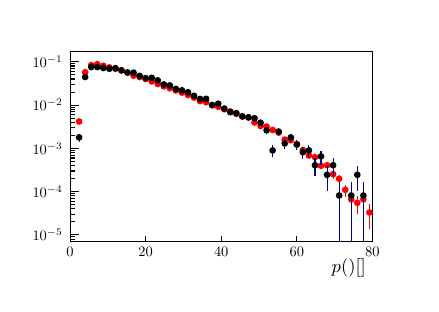
\begin{tikzpicture}
\pgfdeclareplotmark{cross} {
\pgfpathmoveto{\pgfpoint{-0.3\pgfplotmarksize}{\pgfplotmarksize}}
\pgfpathlineto{\pgfpoint{+0.3\pgfplotmarksize}{\pgfplotmarksize}}
\pgfpathlineto{\pgfpoint{+0.3\pgfplotmarksize}{0.3\pgfplotmarksize}}
\pgfpathlineto{\pgfpoint{+1\pgfplotmarksize}{0.3\pgfplotmarksize}}
\pgfpathlineto{\pgfpoint{+1\pgfplotmarksize}{-0.3\pgfplotmarksize}}
\pgfpathlineto{\pgfpoint{+0.3\pgfplotmarksize}{-0.3\pgfplotmarksize}}
\pgfpathlineto{\pgfpoint{+0.3\pgfplotmarksize}{-1.\pgfplotmarksize}}
\pgfpathlineto{\pgfpoint{-0.3\pgfplotmarksize}{-1.\pgfplotmarksize}}
\pgfpathlineto{\pgfpoint{-0.3\pgfplotmarksize}{-0.3\pgfplotmarksize}}
\pgfpathlineto{\pgfpoint{-1.\pgfplotmarksize}{-0.3\pgfplotmarksize}}
\pgfpathlineto{\pgfpoint{-1.\pgfplotmarksize}{0.3\pgfplotmarksize}}
\pgfpathlineto{\pgfpoint{-0.3\pgfplotmarksize}{0.3\pgfplotmarksize}}
\pgfpathclose
\pgfusepathqstroke
}
\pgfdeclareplotmark{cross*} {
\pgfpathmoveto{\pgfpoint{-0.3\pgfplotmarksize}{\pgfplotmarksize}}
\pgfpathlineto{\pgfpoint{+0.3\pgfplotmarksize}{\pgfplotmarksize}}
\pgfpathlineto{\pgfpoint{+0.3\pgfplotmarksize}{0.3\pgfplotmarksize}}
\pgfpathlineto{\pgfpoint{+1\pgfplotmarksize}{0.3\pgfplotmarksize}}
\pgfpathlineto{\pgfpoint{+1\pgfplotmarksize}{-0.3\pgfplotmarksize}}
\pgfpathlineto{\pgfpoint{+0.3\pgfplotmarksize}{-0.3\pgfplotmarksize}}
\pgfpathlineto{\pgfpoint{+0.3\pgfplotmarksize}{-1.\pgfplotmarksize}}
\pgfpathlineto{\pgfpoint{-0.3\pgfplotmarksize}{-1.\pgfplotmarksize}}
\pgfpathlineto{\pgfpoint{-0.3\pgfplotmarksize}{-0.3\pgfplotmarksize}}
\pgfpathlineto{\pgfpoint{-1.\pgfplotmarksize}{-0.3\pgfplotmarksize}}
\pgfpathlineto{\pgfpoint{-1.\pgfplotmarksize}{0.3\pgfplotmarksize}}
\pgfpathlineto{\pgfpoint{-0.3\pgfplotmarksize}{0.3\pgfplotmarksize}}
\pgfpathclose
\pgfusepathqfillstroke
}
\pgfdeclareplotmark{newstar} {
\pgfpathmoveto{\pgfqpoint{0pt}{\pgfplotmarksize}}
\pgfpathlineto{\pgfqpointpolar{44}{0.5\pgfplotmarksize}}
\pgfpathlineto{\pgfqpointpolar{18}{\pgfplotmarksize}}
\pgfpathlineto{\pgfqpointpolar{-20}{0.5\pgfplotmarksize}}
\pgfpathlineto{\pgfqpointpolar{-54}{\pgfplotmarksize}}
\pgfpathlineto{\pgfqpointpolar{-90}{0.5\pgfplotmarksize}}
\pgfpathlineto{\pgfqpointpolar{234}{\pgfplotmarksize}}
\pgfpathlineto{\pgfqpointpolar{198}{0.5\pgfplotmarksize}}
\pgfpathlineto{\pgfqpointpolar{162}{\pgfplotmarksize}}
\pgfpathlineto{\pgfqpointpolar{134}{0.5\pgfplotmarksize}}
\pgfpathclose
\pgfusepathqstroke
}
\pgfdeclareplotmark{newstar*} {
\pgfpathmoveto{\pgfqpoint{0pt}{\pgfplotmarksize}}
\pgfpathlineto{\pgfqpointpolar{44}{0.5\pgfplotmarksize}}
\pgfpathlineto{\pgfqpointpolar{18}{\pgfplotmarksize}}
\pgfpathlineto{\pgfqpointpolar{-20}{0.5\pgfplotmarksize}}
\pgfpathlineto{\pgfqpointpolar{-54}{\pgfplotmarksize}}
\pgfpathlineto{\pgfqpointpolar{-90}{0.5\pgfplotmarksize}}
\pgfpathlineto{\pgfqpointpolar{234}{\pgfplotmarksize}}
\pgfpathlineto{\pgfqpointpolar{198}{0.5\pgfplotmarksize}}
\pgfpathlineto{\pgfqpointpolar{162}{\pgfplotmarksize}}
\pgfpathlineto{\pgfqpointpolar{134}{0.5\pgfplotmarksize}}
\pgfpathclose
\pgfusepathqfillstroke
}
\definecolor{c}{rgb}{1,1,1};
\draw [color=c, fill=c] (0.1,3.20034) rectangle (4.9,6.21242);
\draw [color=c, fill=c] (0.58,3.50154) rectangle (4.42,5.91121);
\definecolor{c}{rgb}{0,0,0};
\draw [c] (0.58,3.50154) -- (0.58,5.91121) -- (4.42,5.91121) -- (4.42,3.50154) -- (0.58,3.50154);
\definecolor{c}{rgb}{1,0,0};
\draw [c] (0.6952,5.01563) -- (0.6952,5.0282);
\draw [c] (0.6952,5.0282) -- (0.6952,5.04014);
\draw [c] (0.6568,5.0282) -- (0.6952,5.0282);
\draw [c] (0.6952,5.0282) -- (0.7336,5.0282);
\foreach \P in {(0.6952,5.0282)}{\draw[mark options={color=c,fill=c},mark size=2.402402pt,mark=*,mark size=1pt] plot coordinates {\P};}
\draw [c] (0.772,5.65055) -- (0.772,5.65387);
\draw [c] (0.772,5.65387) -- (0.772,5.65715);
\draw [c] (0.7336,5.65387) -- (0.772,5.65387);
\draw [c] (0.772,5.65387) -- (0.8104,5.65387);
\foreach \P in {(0.772,5.65387)}{\draw[mark options={color=c,fill=c},mark size=2.402402pt,mark=*,mark size=1pt] plot coordinates {\P};}
\draw [c] (0.8488,5.74086) -- (0.8488,5.74361);
\draw [c] (0.8488,5.74361) -- (0.8488,5.74633);
\draw [c] (0.8104,5.74361) -- (0.8488,5.74361);
\draw [c] (0.8488,5.74361) -- (0.8872,5.74361);
\foreach \P in {(0.8488,5.74361)}{\draw[mark options={color=c,fill=c},mark size=2.402402pt,mark=*,mark size=1pt] plot coordinates {\P};}
\draw [c] (0.9256,5.75333) -- (0.9256,5.75601);
\draw [c] (0.9256,5.75601) -- (0.9256,5.75866);
\draw [c] (0.8872,5.75601) -- (0.9256,5.75601);
\draw [c] (0.9256,5.75601) -- (0.964,5.75601);
\foreach \P in {(0.9256,5.75601)}{\draw[mark options={color=c,fill=c},mark size=2.402402pt,mark=*,mark size=1pt] plot coordinates {\P};}
\draw [c] (1.0024,5.73281) -- (1.0024,5.7356);
\draw [c] (1.0024,5.7356) -- (1.0024,5.73837);
\draw [c] (0.964,5.7356) -- (1.0024,5.7356);
\draw [c] (1.0024,5.7356) -- (1.0408,5.7356);
\foreach \P in {(1.0024,5.7356)}{\draw[mark options={color=c,fill=c},mark size=2.402402pt,mark=*,mark size=1pt] plot coordinates {\P};}
\draw [c] (1.0792,5.71214) -- (1.0792,5.71506);
\draw [c] (1.0792,5.71506) -- (1.0792,5.71795);
\draw [c] (1.0408,5.71506) -- (1.0792,5.71506);
\draw [c] (1.0792,5.71506) -- (1.1176,5.71506);
\foreach \P in {(1.0792,5.71506)}{\draw[mark options={color=c,fill=c},mark size=2.402402pt,mark=*,mark size=1pt] plot coordinates {\P};}
\draw [c] (1.156,5.69412) -- (1.156,5.69715);
\draw [c] (1.156,5.69715) -- (1.156,5.70015);
\draw [c] (1.1176,5.69715) -- (1.156,5.69715);
\draw [c] (1.156,5.69715) -- (1.1944,5.69715);
\foreach \P in {(1.156,5.69715)}{\draw[mark options={color=c,fill=c},mark size=2.402402pt,mark=*,mark size=1pt] plot coordinates {\P};}
\draw [c] (1.2328,5.67455) -- (1.2328,5.67772);
\draw [c] (1.2328,5.67772) -- (1.2328,5.68084);
\draw [c] (1.1944,5.67772) -- (1.2328,5.67772);
\draw [c] (1.2328,5.67772) -- (1.2712,5.67772);
\foreach \P in {(1.2328,5.67772)}{\draw[mark options={color=c,fill=c},mark size=2.402402pt,mark=*,mark size=1pt] plot coordinates {\P};}
\draw [c] (1.3096,5.64468) -- (1.3096,5.64805);
\draw [c] (1.3096,5.64805) -- (1.3096,5.65137);
\draw [c] (1.2712,5.64805) -- (1.3096,5.64805);
\draw [c] (1.3096,5.64805) -- (1.348,5.64805);
\foreach \P in {(1.3096,5.64805)}{\draw[mark options={color=c,fill=c},mark size=2.402402pt,mark=*,mark size=1pt] plot coordinates {\P};}
\draw [c] (1.3864,5.60566) -- (1.3864,5.60931);
\draw [c] (1.3864,5.60931) -- (1.3864,5.61291);
\draw [c] (1.348,5.60931) -- (1.3864,5.60931);
\draw [c] (1.3864,5.60931) -- (1.4248,5.60931);
\foreach \P in {(1.3864,5.60931)}{\draw[mark options={color=c,fill=c},mark size=2.402402pt,mark=*,mark size=1pt] plot coordinates {\P};}
\draw [c] (1.4632,5.58877) -- (1.4632,5.59255);
\draw [c] (1.4632,5.59255) -- (1.4632,5.59628);
\draw [c] (1.4248,5.59255) -- (1.4632,5.59255);
\draw [c] (1.4632,5.59255) -- (1.5016,5.59255);
\foreach \P in {(1.4632,5.59255)}{\draw[mark options={color=c,fill=c},mark size=2.402402pt,mark=*,mark size=1pt] plot coordinates {\P};}
\draw [c] (1.54,5.56336) -- (1.54,5.56735);
\draw [c] (1.54,5.56735) -- (1.54,5.57127);
\draw [c] (1.5016,5.56735) -- (1.54,5.56735);
\draw [c] (1.54,5.56735) -- (1.5784,5.56735);
\foreach \P in {(1.54,5.56735)}{\draw[mark options={color=c,fill=c},mark size=2.402402pt,mark=*,mark size=1pt] plot coordinates {\P};}
\draw [c] (1.6168,5.53291) -- (1.6168,5.53717);
\draw [c] (1.6168,5.53717) -- (1.6168,5.54135);
\draw [c] (1.5784,5.53717) -- (1.6168,5.53717);
\draw [c] (1.6168,5.53717) -- (1.6552,5.53717);
\foreach \P in {(1.6168,5.53717)}{\draw[mark options={color=c,fill=c},mark size=2.402402pt,mark=*,mark size=1pt] plot coordinates {\P};}
\draw [c] (1.6936,5.49985) -- (1.6936,5.50441);
\draw [c] (1.6936,5.50441) -- (1.6936,5.50888);
\draw [c] (1.6552,5.50441) -- (1.6936,5.50441);
\draw [c] (1.6936,5.50441) -- (1.732,5.50441);
\foreach \P in {(1.6936,5.50441)}{\draw[mark options={color=c,fill=c},mark size=2.402402pt,mark=*,mark size=1pt] plot coordinates {\P};}
\draw [c] (1.7704,5.46945) -- (1.7704,5.47431);
\draw [c] (1.7704,5.47431) -- (1.7704,5.47907);
\draw [c] (1.732,5.47431) -- (1.7704,5.47431);
\draw [c] (1.7704,5.47431) -- (1.8088,5.47431);
\foreach \P in {(1.7704,5.47431)}{\draw[mark options={color=c,fill=c},mark size=2.402402pt,mark=*,mark size=1pt] plot coordinates {\P};}
\draw [c] (1.8472,5.44494) -- (1.8472,5.45006);
\draw [c] (1.8472,5.45006) -- (1.8472,5.45506);
\draw [c] (1.8088,5.45006) -- (1.8472,5.45006);
\draw [c] (1.8472,5.45006) -- (1.8856,5.45006);
\foreach \P in {(1.8472,5.45006)}{\draw[mark options={color=c,fill=c},mark size=2.402402pt,mark=*,mark size=1pt] plot coordinates {\P};}
\draw [c] (1.924,5.41617) -- (1.924,5.42161);
\draw [c] (1.924,5.42161) -- (1.924,5.42692);
\draw [c] (1.8856,5.42161) -- (1.924,5.42161);
\draw [c] (1.924,5.42161) -- (1.9624,5.42161);
\foreach \P in {(1.924,5.42161)}{\draw[mark options={color=c,fill=c},mark size=2.402402pt,mark=*,mark size=1pt] plot coordinates {\P};}
\draw [c] (2.0008,5.38861) -- (2.0008,5.39437);
\draw [c] (2.0008,5.39437) -- (2.0008,5.39999);
\draw [c] (1.9624,5.39437) -- (2.0008,5.39437);
\draw [c] (2.0008,5.39437) -- (2.0392,5.39437);
\foreach \P in {(2.0008,5.39437)}{\draw[mark options={color=c,fill=c},mark size=2.402402pt,mark=*,mark size=1pt] plot coordinates {\P};}
\draw [c] (2.0776,5.35794) -- (2.0776,5.36407);
\draw [c] (2.0776,5.36407) -- (2.0776,5.37006);
\draw [c] (2.0392,5.36407) -- (2.0776,5.36407);
\draw [c] (2.0776,5.36407) -- (2.116,5.36407);
\foreach \P in {(2.0776,5.36407)}{\draw[mark options={color=c,fill=c},mark size=2.402402pt,mark=*,mark size=1pt] plot coordinates {\P};}
\draw [c] (2.1544,5.32421) -- (2.1544,5.33079);
\draw [c] (2.1544,5.33079) -- (2.1544,5.3372);
\draw [c] (2.116,5.33079) -- (2.1544,5.33079);
\draw [c] (2.1544,5.33079) -- (2.1928,5.33079);
\foreach \P in {(2.1544,5.33079)}{\draw[mark options={color=c,fill=c},mark size=2.402402pt,mark=*,mark size=1pt] plot coordinates {\P};}
\draw [c] (2.2312,5.27897) -- (2.2312,5.28621);
\draw [c] (2.2312,5.28621) -- (2.2312,5.29324);
\draw [c] (2.1928,5.28621) -- (2.2312,5.28621);
\draw [c] (2.2312,5.28621) -- (2.2696,5.28621);
\foreach \P in {(2.2312,5.28621)}{\draw[mark options={color=c,fill=c},mark size=2.402402pt,mark=*,mark size=1pt] plot coordinates {\P};}
\draw [c] (2.308,5.26516) -- (2.308,5.27262);
\draw [c] (2.308,5.27262) -- (2.308,5.27984);
\draw [c] (2.2696,5.27262) -- (2.308,5.27262);
\draw [c] (2.308,5.27262) -- (2.3464,5.27262);
\foreach \P in {(2.308,5.27262)}{\draw[mark options={color=c,fill=c},mark size=2.402402pt,mark=*,mark size=1pt] plot coordinates {\P};}
\draw [c] (2.3848,5.22565) -- (2.3848,5.23374);
\draw [c] (2.3848,5.23374) -- (2.3848,5.24158);
\draw [c] (2.3464,5.23374) -- (2.3848,5.23374);
\draw [c] (2.3848,5.23374) -- (2.4232,5.23374);
\foreach \P in {(2.3848,5.23374)}{\draw[mark options={color=c,fill=c},mark size=2.402402pt,mark=*,mark size=1pt] plot coordinates {\P};}
\draw [c] (2.4616,5.20566) -- (2.4616,5.21411);
\draw [c] (2.4616,5.21411) -- (2.4616,5.22226);
\draw [c] (2.4232,5.21411) -- (2.4616,5.21411);
\draw [c] (2.4616,5.21411) -- (2.5,5.21411);
\foreach \P in {(2.4616,5.21411)}{\draw[mark options={color=c,fill=c},mark size=2.402402pt,mark=*,mark size=1pt] plot coordinates {\P};}
\draw [c] (2.5384,5.17437) -- (2.5384,5.18338);
\draw [c] (2.5384,5.18338) -- (2.5384,5.19207);
\draw [c] (2.5,5.18338) -- (2.5384,5.18338);
\draw [c] (2.5384,5.18338) -- (2.5768,5.18338);
\foreach \P in {(2.5384,5.18338)}{\draw[mark options={color=c,fill=c},mark size=2.402402pt,mark=*,mark size=1pt] plot coordinates {\P};}
\draw [c] (2.6152,5.14603) -- (2.6152,5.1556);
\draw [c] (2.6152,5.1556) -- (2.6152,5.1648);
\draw [c] (2.5768,5.1556) -- (2.6152,5.1556);
\draw [c] (2.6152,5.1556) -- (2.6536,5.1556);
\foreach \P in {(2.6152,5.1556)}{\draw[mark options={color=c,fill=c},mark size=2.402402pt,mark=*,mark size=1pt] plot coordinates {\P};}
\draw [c] (2.692,5.11434) -- (2.692,5.12457);
\draw [c] (2.692,5.12457) -- (2.692,5.13437);
\draw [c] (2.6536,5.12457) -- (2.692,5.12457);
\draw [c] (2.692,5.12457) -- (2.7304,5.12457);
\foreach \P in {(2.692,5.12457)}{\draw[mark options={color=c,fill=c},mark size=2.402402pt,mark=*,mark size=1pt] plot coordinates {\P};}
\draw [c] (2.7688,5.07984) -- (2.7688,5.09083);
\draw [c] (2.7688,5.09083) -- (2.7688,5.10133);
\draw [c] (2.7304,5.09083) -- (2.7688,5.09083);
\draw [c] (2.7688,5.09083) -- (2.8072,5.09083);
\foreach \P in {(2.7688,5.09083)}{\draw[mark options={color=c,fill=c},mark size=2.402402pt,mark=*,mark size=1pt] plot coordinates {\P};}
\draw [c] (2.8456,5.06767) -- (2.8456,5.07894);
\draw [c] (2.8456,5.07894) -- (2.8456,5.0897);
\draw [c] (2.8072,5.07894) -- (2.8456,5.07894);
\draw [c] (2.8456,5.07894) -- (2.884,5.07894);
\foreach \P in {(2.8456,5.07894)}{\draw[mark options={color=c,fill=c},mark size=2.402402pt,mark=*,mark size=1pt] plot coordinates {\P};}
\draw [c] (2.9224,5.00305) -- (2.9224,5.01596);
\draw [c] (2.9224,5.01596) -- (2.9224,5.0282);
\draw [c] (2.884,5.01596) -- (2.9224,5.01596);
\draw [c] (2.9224,5.01596) -- (2.9608,5.01596);
\foreach \P in {(2.9224,5.01596)}{\draw[mark options={color=c,fill=c},mark size=2.402402pt,mark=*,mark size=1pt] plot coordinates {\P};}
\draw [c] (2.9992,4.95676) -- (2.9992,4.97098);
\draw [c] (2.9992,4.97098) -- (2.9992,4.9844);
\draw [c] (2.9608,4.97098) -- (2.9992,4.97098);
\draw [c] (2.9992,4.97098) -- (3.0376,4.97098);
\foreach \P in {(2.9992,4.97098)}{\draw[mark options={color=c,fill=c},mark size=2.402402pt,mark=*,mark size=1pt] plot coordinates {\P};}
\draw [c] (3.076,4.94839) -- (3.076,4.96286);
\draw [c] (3.076,4.96286) -- (3.076,4.97651);
\draw [c] (3.0376,4.96286) -- (3.076,4.96286);
\draw [c] (3.076,4.96286) -- (3.1144,4.96286);
\foreach \P in {(3.076,4.96286)}{\draw[mark options={color=c,fill=c},mark size=2.402402pt,mark=*,mark size=1pt] plot coordinates {\P};}
\draw [c] (3.1528,4.90464) -- (3.1528,4.9205);
\draw [c] (3.1528,4.9205) -- (3.1528,4.93537);
\draw [c] (3.1144,4.9205) -- (3.1528,4.9205);
\draw [c] (3.1528,4.9205) -- (3.1912,4.9205);
\foreach \P in {(3.1528,4.9205)}{\draw[mark options={color=c,fill=c},mark size=2.402402pt,mark=*,mark size=1pt] plot coordinates {\P};}
\draw [c] (3.2296,4.86839) -- (3.2296,4.8855);
\draw [c] (3.2296,4.8855) -- (3.2296,4.90147);
\draw [c] (3.1912,4.8855) -- (3.2296,4.8855);
\draw [c] (3.2296,4.8855) -- (3.268,4.8855);
\foreach \P in {(3.2296,4.8855)}{\draw[mark options={color=c,fill=c},mark size=2.402402pt,mark=*,mark size=1pt] plot coordinates {\P};}
\draw [c] (3.3064,4.77754) -- (3.3064,4.79824);
\draw [c] (3.3064,4.79824) -- (3.3064,4.81728);
\draw [c] (3.268,4.79824) -- (3.3064,4.79824);
\draw [c] (3.3064,4.79824) -- (3.3448,4.79824);
\foreach \P in {(3.3064,4.79824)}{\draw[mark options={color=c,fill=c},mark size=2.402402pt,mark=*,mark size=1pt] plot coordinates {\P};}
\draw [c] (3.3832,4.76878) -- (3.3832,4.78986);
\draw [c] (3.3832,4.78986) -- (3.3832,4.80923);
\draw [c] (3.3448,4.78986) -- (3.3832,4.78986);
\draw [c] (3.3832,4.78986) -- (3.4216,4.78986);
\foreach \P in {(3.3832,4.78986)}{\draw[mark options={color=c,fill=c},mark size=2.402402pt,mark=*,mark size=1pt] plot coordinates {\P};}
\draw [c] (3.46,4.71954) -- (3.46,4.74291);
\draw [c] (3.46,4.74291) -- (3.46,4.76419);
\draw [c] (3.4216,4.74291) -- (3.46,4.74291);
\draw [c] (3.46,4.74291) -- (3.4984,4.74291);
\foreach \P in {(3.46,4.74291)}{\draw[mark options={color=c,fill=c},mark size=2.402402pt,mark=*,mark size=1pt] plot coordinates {\P};}
\draw [c] (3.5368,4.63732) -- (3.5368,4.66507);
\draw [c] (3.5368,4.66507) -- (3.5368,4.68993);
\draw [c] (3.4984,4.66507) -- (3.5368,4.66507);
\draw [c] (3.5368,4.66507) -- (3.5752,4.66507);
\foreach \P in {(3.5368,4.66507)}{\draw[mark options={color=c,fill=c},mark size=2.402402pt,mark=*,mark size=1pt] plot coordinates {\P};}
\draw [c] (3.6136,4.56303) -- (3.6136,4.59544);
\draw [c] (3.6136,4.59544) -- (3.6136,4.62398);
\draw [c] (3.5752,4.59544) -- (3.6136,4.59544);
\draw [c] (3.6136,4.59544) -- (3.652,4.59544);
\foreach \P in {(3.6136,4.59544)}{\draw[mark options={color=c,fill=c},mark size=2.402402pt,mark=*,mark size=1pt] plot coordinates {\P};}
\draw [c] (3.6904,4.54146) -- (3.6904,4.57537);
\draw [c] (3.6904,4.57537) -- (3.6904,4.60506);
\draw [c] (3.652,4.57537) -- (3.6904,4.57537);
\draw [c] (3.6904,4.57537) -- (3.7288,4.57537);
\foreach \P in {(3.6904,4.57537)}{\draw[mark options={color=c,fill=c},mark size=2.402402pt,mark=*,mark size=1pt] plot coordinates {\P};}
\draw [c] (3.7672,4.42217) -- (3.7672,4.46569);
\draw [c] (3.7672,4.46569) -- (3.7672,4.50248);
\draw [c] (3.7288,4.46569) -- (3.7672,4.46569);
\draw [c] (3.7672,4.46569) -- (3.8056,4.46569);
\foreach \P in {(3.7672,4.46569)}{\draw[mark options={color=c,fill=c},mark size=2.402402pt,mark=*,mark size=1pt] plot coordinates {\P};}
\draw [c] (3.844,4.42936) -- (3.844,4.47223);
\draw [c] (3.844,4.47223) -- (3.844,4.50856);
\draw [c] (3.8056,4.47223) -- (3.844,4.47223);
\draw [c] (3.844,4.47223) -- (3.8824,4.47223);
\foreach \P in {(3.844,4.47223)}{\draw[mark options={color=c,fill=c},mark size=2.402402pt,mark=*,mark size=1pt] plot coordinates {\P};}
\draw [c] (3.9208,4.30293) -- (3.9208,4.35875);
\draw [c] (3.9208,4.35875) -- (3.9208,4.40395);
\draw [c] (3.8824,4.35875) -- (3.9208,4.35875);
\draw [c] (3.9208,4.35875) -- (3.9592,4.35875);
\foreach \P in {(3.9208,4.35875)}{\draw[mark options={color=c,fill=c},mark size=2.402402pt,mark=*,mark size=1pt] plot coordinates {\P};}
\draw [c] (3.9976,4.23608) -- (3.9976,4.30024);
\draw [c] (3.9976,4.30024) -- (3.9976,4.35076);
\draw [c] (3.9592,4.30024) -- (3.9976,4.30024);
\draw [c] (3.9976,4.30024) -- (4.036,4.30024);
\foreach \P in {(3.9976,4.30024)}{\draw[mark options={color=c,fill=c},mark size=2.402402pt,mark=*,mark size=1pt] plot coordinates {\P};}
\draw [c] (4.0744,4.0692) -- (4.0744,4.15994);
\draw [c] (4.0744,4.15994) -- (4.0744,4.22552);
\draw [c] (4.036,4.15994) -- (4.0744,4.15994);
\draw [c] (4.0744,4.15994) -- (4.1128,4.15994);
\foreach \P in {(4.0744,4.15994)}{\draw[mark options={color=c,fill=c},mark size=2.402402pt,mark=*,mark size=1pt] plot coordinates {\P};}
\draw [c] (4.1512,3.91277) -- (4.1512,4.03801);
\draw [c] (4.1512,4.03801) -- (4.1512,4.11972);
\draw [c] (4.1128,4.03801) -- (4.1512,4.03801);
\draw [c] (4.1512,4.03801) -- (4.1896,4.03801);
\foreach \P in {(4.1512,4.03801)}{\draw[mark options={color=c,fill=c},mark size=2.402402pt,mark=*,mark size=1pt] plot coordinates {\P};}
\draw [c] (4.228,3.853) -- (4.228,3.99449);
\draw [c] (4.228,3.99449) -- (4.228,4.08272);
\draw [c] (4.1896,3.99449) -- (4.228,3.99449);
\draw [c] (4.228,3.99449) -- (4.2664,3.99449);
\foreach \P in {(4.228,3.99449)}{\draw[mark options={color=c,fill=c},mark size=2.402402pt,mark=*,mark size=1pt] plot coordinates {\P};}
\draw [c] (4.3048,3.91277) -- (4.3048,4.03801);
\draw [c] (4.3048,4.03801) -- (4.3048,4.11972);
\draw [c] (4.2664,4.03801) -- (4.3048,4.03801);
\draw [c] (4.3048,4.03801) -- (4.3432,4.03801);
\foreach \P in {(4.3048,4.03801)}{\draw[mark options={color=c,fill=c},mark size=2.402402pt,mark=*,mark size=1pt] plot coordinates {\P};}
\draw [c] (4.3816,3.66699) -- (4.3816,3.87256);
\draw [c] (4.3816,3.87256) -- (4.3816,3.98134);
\draw [c] (4.3432,3.87256) -- (4.3816,3.87256);
\draw [c] (4.3816,3.87256) -- (4.42,3.87256);
\foreach \P in {(4.3816,3.87256)}{\draw[mark options={color=c,fill=c},mark size=2.402402pt,mark=*,mark size=1pt] plot coordinates {\P};}
\definecolor{c}{rgb}{0,0,0};
\draw [c] (0.58,3.50154) -- (4.42,3.50154);
\draw [anchor= east] (4.42,3.16419) node[scale=0.672711, rotate=0]{$p(\kaon) [\mevc]$};
\draw [c] (0.58,3.57383) -- (0.58,3.50154);
\draw [c] (1.54,3.57383) -- (1.54,3.50154);
\draw [c] (2.5,3.57383) -- (2.5,3.50154);
\draw [c] (3.46,3.57383) -- (3.46,3.50154);
\draw [c] (4.42,3.57383) -- (4.42,3.50154);
\draw [anchor=base] (0.58,3.30877) node[scale=0.52322, rotate=0]{0};
\draw [anchor=base] (1.54,3.30877) node[scale=0.52322, rotate=0]{20};
\draw [anchor=base] (2.5,3.30877) node[scale=0.52322, rotate=0]{40};
\draw [anchor=base] (3.46,3.30877) node[scale=0.52322, rotate=0]{60};
\draw [anchor=base] (4.42,3.30877) node[scale=0.52322, rotate=0]{80};
\draw [c] (0.58,3.50154) -- (0.58,5.91121);
\draw [c] (0.6376,3.50214) -- (0.58,3.50214);
\draw [c] (0.6376,3.53402) -- (0.58,3.53402);
\draw [c] (0.6376,3.56213) -- (0.58,3.56213);
\draw [c] (0.6952,3.58728) -- (0.58,3.58728);
\draw [anchor= east] (0.54928,3.58728) node[scale=0.52322, rotate=0]{$10^{-5}$};
\draw [c] (0.6376,3.75273) -- (0.58,3.75273);
\draw [c] (0.6376,3.84951) -- (0.58,3.84951);
\draw [c] (0.6376,3.91818) -- (0.58,3.91818);
\draw [c] (0.6376,3.97144) -- (0.58,3.97144);
\draw [c] (0.6376,4.01496) -- (0.58,4.01496);
\draw [c] (0.6376,4.05175) -- (0.58,4.05175);
\draw [c] (0.6376,4.08363) -- (0.58,4.08363);
\draw [c] (0.6376,4.11174) -- (0.58,4.11174);
\draw [c] (0.6952,4.13689) -- (0.58,4.13689);
\draw [anchor= east] (0.54928,4.13689) node[scale=0.52322, rotate=0]{$10^{-4}$};
\draw [c] (0.6376,4.30234) -- (0.58,4.30234);
\draw [c] (0.6376,4.39912) -- (0.58,4.39912);
\draw [c] (0.6376,4.46779) -- (0.58,4.46779);
\draw [c] (0.6376,4.52105) -- (0.58,4.52105);
\draw [c] (0.6376,4.56457) -- (0.58,4.56457);
\draw [c] (0.6376,4.60136) -- (0.58,4.60136);
\draw [c] (0.6376,4.63324) -- (0.58,4.63324);
\draw [c] (0.6376,4.66135) -- (0.58,4.66135);
\draw [c] (0.6952,4.6865) -- (0.58,4.6865);
\draw [anchor= east] (0.54928,4.6865) node[scale=0.52322, rotate=0]{$10^{-3}$};
\draw [c] (0.6376,4.85195) -- (0.58,4.85195);
\draw [c] (0.6376,4.94873) -- (0.58,4.94873);
\draw [c] (0.6376,5.0174) -- (0.58,5.0174);
\draw [c] (0.6376,5.07066) -- (0.58,5.07066);
\draw [c] (0.6376,5.11418) -- (0.58,5.11418);
\draw [c] (0.6376,5.15097) -- (0.58,5.15097);
\draw [c] (0.6376,5.18285) -- (0.58,5.18285);
\draw [c] (0.6376,5.21096) -- (0.58,5.21096);
\draw [c] (0.6952,5.23611) -- (0.58,5.23611);
\draw [anchor= east] (0.54928,5.23611) node[scale=0.52322, rotate=0]{$10^{-2}$};
\draw [c] (0.6376,5.40156) -- (0.58,5.40156);
\draw [c] (0.6376,5.49834) -- (0.58,5.49834);
\draw [c] (0.6376,5.56701) -- (0.58,5.56701);
\draw [c] (0.6376,5.62027) -- (0.58,5.62027);
\draw [c] (0.6376,5.66379) -- (0.58,5.66379);
\draw [c] (0.6376,5.70058) -- (0.58,5.70058);
\draw [c] (0.6376,5.73246) -- (0.58,5.73246);
\draw [c] (0.6376,5.76057) -- (0.58,5.76057);
\draw [c] (0.6952,5.78572) -- (0.58,5.78572);
\draw [anchor= east] (0.54928,5.78572) node[scale=0.52322, rotate=0]{$10^{-1}$};
\definecolor{c}{rgb}{0,0,0.6};
\draw [c] (0.6952,4.76891) -- (0.6952,4.82614);
\draw [c] (0.6952,4.82614) -- (0.6952,4.87227);
\draw [c] (0.6568,4.82614) -- (0.6952,4.82614);
\draw [c] (0.6952,4.82614) -- (0.7336,4.82614);
\definecolor{c}{rgb}{0,0,0};
\foreach \P in {(0.6952,4.82614)}{\draw[mark options={color=c,fill=c},mark size=2.402402pt,mark=*,mark size=1pt] plot coordinates {\P};}
\definecolor{c}{rgb}{0,0,0.6};
\draw [c] (0.772,5.58273) -- (0.772,5.59316);
\draw [c] (0.772,5.59316) -- (0.772,5.60315);
\draw [c] (0.7336,5.59316) -- (0.772,5.59316);
\draw [c] (0.772,5.59316) -- (0.8104,5.59316);
\definecolor{c}{rgb}{0,0,0};
\foreach \P in {(0.772,5.59316)}{\draw[mark options={color=c,fill=c},mark size=2.402402pt,mark=*,mark size=1pt] plot coordinates {\P};}
\definecolor{c}{rgb}{0,0,0.6};
\draw [c] (0.8488,5.71136) -- (0.8488,5.71933);
\draw [c] (0.8488,5.71933) -- (0.8488,5.72704);
\draw [c] (0.8104,5.71933) -- (0.8488,5.71933);
\draw [c] (0.8488,5.71933) -- (0.8872,5.71933);
\definecolor{c}{rgb}{0,0,0};
\foreach \P in {(0.8488,5.71933)}{\draw[mark options={color=c,fill=c},mark size=2.402402pt,mark=*,mark size=1pt] plot coordinates {\P};}
\definecolor{c}{rgb}{0,0,0.6};
\draw [c] (0.9256,5.71136) -- (0.9256,5.71933);
\draw [c] (0.9256,5.71933) -- (0.9256,5.72704);
\draw [c] (0.8872,5.71933) -- (0.9256,5.71933);
\draw [c] (0.9256,5.71933) -- (0.964,5.71933);
\definecolor{c}{rgb}{0,0,0};
\foreach \P in {(0.9256,5.71933)}{\draw[mark options={color=c,fill=c},mark size=2.402402pt,mark=*,mark size=1pt] plot coordinates {\P};}
\definecolor{c}{rgb}{0,0,0.6};
\draw [c] (1.0024,5.69874) -- (1.0024,5.70692);
\draw [c] (1.0024,5.70692) -- (1.0024,5.71483);
\draw [c] (0.964,5.70692) -- (1.0024,5.70692);
\draw [c] (1.0024,5.70692) -- (1.0408,5.70692);
\definecolor{c}{rgb}{0,0,0};
\foreach \P in {(1.0024,5.70692)}{\draw[mark options={color=c,fill=c},mark size=2.402402pt,mark=*,mark size=1pt] plot coordinates {\P};}
\definecolor{c}{rgb}{0,0,0.6};
\draw [c] (1.0792,5.68918) -- (1.0792,5.69753);
\draw [c] (1.0792,5.69753) -- (1.0792,5.70559);
\draw [c] (1.0408,5.69753) -- (1.0792,5.69753);
\draw [c] (1.0792,5.69753) -- (1.1176,5.69753);
\definecolor{c}{rgb}{0,0,0};
\foreach \P in {(1.0792,5.69753)}{\draw[mark options={color=c,fill=c},mark size=2.402402pt,mark=*,mark size=1pt] plot coordinates {\P};}
\definecolor{c}{rgb}{0,0,0.6};
\draw [c] (1.156,5.6968) -- (1.156,5.70502);
\draw [c] (1.156,5.70502) -- (1.156,5.71296);
\draw [c] (1.1176,5.70502) -- (1.156,5.70502);
\draw [c] (1.156,5.70502) -- (1.1944,5.70502);
\definecolor{c}{rgb}{0,0,0};
\foreach \P in {(1.156,5.70502)}{\draw[mark options={color=c,fill=c},mark size=2.402402pt,mark=*,mark size=1pt] plot coordinates {\P};}
\definecolor{c}{rgb}{0,0,0.6};
\draw [c] (1.2328,5.6679) -- (1.2328,5.67663);
\draw [c] (1.2328,5.67663) -- (1.2328,5.68505);
\draw [c] (1.1944,5.67663) -- (1.2328,5.67663);
\draw [c] (1.2328,5.67663) -- (1.2712,5.67663);
\definecolor{c}{rgb}{0,0,0};
\foreach \P in {(1.2328,5.67663)}{\draw[mark options={color=c,fill=c},mark size=2.402402pt,mark=*,mark size=1pt] plot coordinates {\P};}
\definecolor{c}{rgb}{0,0,0.6};
\draw [c] (1.3096,5.64109) -- (1.3096,5.65032);
\draw [c] (1.3096,5.65032) -- (1.3096,5.6592);
\draw [c] (1.2712,5.65032) -- (1.3096,5.65032);
\draw [c] (1.3096,5.65032) -- (1.348,5.65032);
\definecolor{c}{rgb}{0,0,0};
\foreach \P in {(1.3096,5.65032)}{\draw[mark options={color=c,fill=c},mark size=2.402402pt,mark=*,mark size=1pt] plot coordinates {\P};}
\definecolor{c}{rgb}{0,0,0.6};
\draw [c] (1.3864,5.63862) -- (1.3864,5.6479);
\draw [c] (1.3864,5.6479) -- (1.3864,5.65683);
\draw [c] (1.348,5.6479) -- (1.3864,5.6479);
\draw [c] (1.3864,5.6479) -- (1.4248,5.6479);
\definecolor{c}{rgb}{0,0,0};
\foreach \P in {(1.3864,5.6479)}{\draw[mark options={color=c,fill=c},mark size=2.402402pt,mark=*,mark size=1pt] plot coordinates {\P};}
\definecolor{c}{rgb}{0,0,0.6};
\draw [c] (1.4632,5.59702) -- (1.4632,5.60714);
\draw [c] (1.4632,5.60714) -- (1.4632,5.61685);
\draw [c] (1.4248,5.60714) -- (1.4632,5.60714);
\draw [c] (1.4632,5.60714) -- (1.5016,5.60714);
\definecolor{c}{rgb}{0,0,0};
\foreach \P in {(1.4632,5.60714)}{\draw[mark options={color=c,fill=c},mark size=2.402402pt,mark=*,mark size=1pt] plot coordinates {\P};}
\definecolor{c}{rgb}{0,0,0.6};
\draw [c] (1.54,5.56754) -- (1.54,5.5783);
\draw [c] (1.54,5.5783) -- (1.54,5.58861);
\draw [c] (1.5016,5.5783) -- (1.54,5.5783);
\draw [c] (1.54,5.5783) -- (1.5784,5.5783);
\definecolor{c}{rgb}{0,0,0};
\foreach \P in {(1.54,5.5783)}{\draw[mark options={color=c,fill=c},mark size=2.402402pt,mark=*,mark size=1pt] plot coordinates {\P};}
\definecolor{c}{rgb}{0,0,0.6};
\draw [c] (1.6168,5.57178) -- (1.6168,5.58245);
\draw [c] (1.6168,5.58245) -- (1.6168,5.59266);
\draw [c] (1.5784,5.58245) -- (1.6168,5.58245);
\draw [c] (1.6168,5.58245) -- (1.6552,5.58245);
\definecolor{c}{rgb}{0,0,0};
\foreach \P in {(1.6168,5.58245)}{\draw[mark options={color=c,fill=c},mark size=2.402402pt,mark=*,mark size=1pt] plot coordinates {\P};}
\definecolor{c}{rgb}{0,0,0.6};
\draw [c] (1.6936,5.53881) -- (1.6936,5.55025);
\draw [c] (1.6936,5.55025) -- (1.6936,5.56116);
\draw [c] (1.6552,5.55025) -- (1.6936,5.55025);
\draw [c] (1.6936,5.55025) -- (1.732,5.55025);
\definecolor{c}{rgb}{0,0,0};
\foreach \P in {(1.6936,5.55025)}{\draw[mark options={color=c,fill=c},mark size=2.402402pt,mark=*,mark size=1pt] plot coordinates {\P};}
\definecolor{c}{rgb}{0,0,0.6};
\draw [c] (1.7704,5.48577) -- (1.7704,5.49855);
\draw [c] (1.7704,5.49855) -- (1.7704,5.51068);
\draw [c] (1.732,5.49855) -- (1.7704,5.49855);
\draw [c] (1.7704,5.49855) -- (1.8088,5.49855);
\definecolor{c}{rgb}{0,0,0};
\foreach \P in {(1.7704,5.49855)}{\draw[mark options={color=c,fill=c},mark size=2.402402pt,mark=*,mark size=1pt] plot coordinates {\P};}
\definecolor{c}{rgb}{0,0,0.6};
\draw [c] (1.8472,5.47276) -- (1.8472,5.48589);
\draw [c] (1.8472,5.48589) -- (1.8472,5.49834);
\draw [c] (1.8088,5.48589) -- (1.8472,5.48589);
\draw [c] (1.8472,5.48589) -- (1.8856,5.48589);
\definecolor{c}{rgb}{0,0,0};
\foreach \P in {(1.8472,5.48589)}{\draw[mark options={color=c,fill=c},mark size=2.402402pt,mark=*,mark size=1pt] plot coordinates {\P};}
\definecolor{c}{rgb}{0,0,0.6};
\draw [c] (1.924,5.42725) -- (1.924,5.44169);
\draw [c] (1.924,5.44169) -- (1.924,5.45531);
\draw [c] (1.8856,5.44169) -- (1.924,5.44169);
\draw [c] (1.924,5.44169) -- (1.9624,5.44169);
\definecolor{c}{rgb}{0,0,0};
\foreach \P in {(1.924,5.44169)}{\draw[mark options={color=c,fill=c},mark size=2.402402pt,mark=*,mark size=1pt] plot coordinates {\P};}
\definecolor{c}{rgb}{0,0,0.6};
\draw [c] (2.0008,5.40873) -- (2.0008,5.42375);
\draw [c] (2.0008,5.42375) -- (2.0008,5.43788);
\draw [c] (1.9624,5.42375) -- (2.0008,5.42375);
\draw [c] (2.0008,5.42375) -- (2.0392,5.42375);
\definecolor{c}{rgb}{0,0,0};
\foreach \P in {(2.0008,5.42375)}{\draw[mark options={color=c,fill=c},mark size=2.402402pt,mark=*,mark size=1pt] plot coordinates {\P};}
\definecolor{c}{rgb}{0,0,0.6};
\draw [c] (2.0776,5.38366) -- (2.0776,5.39949);
\draw [c] (2.0776,5.39949) -- (2.0776,5.41433);
\draw [c] (2.0392,5.39949) -- (2.0776,5.39949);
\draw [c] (2.0776,5.39949) -- (2.116,5.39949);
\definecolor{c}{rgb}{0,0,0};
\foreach \P in {(2.0776,5.39949)}{\draw[mark options={color=c,fill=c},mark size=2.402402pt,mark=*,mark size=1pt] plot coordinates {\P};}
\definecolor{c}{rgb}{0,0,0.6};
\draw [c] (2.1544,5.33673) -- (2.1544,5.35419);
\draw [c] (2.1544,5.35419) -- (2.1544,5.37046);
\draw [c] (2.116,5.35419) -- (2.1544,5.35419);
\draw [c] (2.1544,5.35419) -- (2.1928,5.35419);
\definecolor{c}{rgb}{0,0,0};
\foreach \P in {(2.1544,5.35419)}{\draw[mark options={color=c,fill=c},mark size=2.402402pt,mark=*,mark size=1pt] plot coordinates {\P};}
\definecolor{c}{rgb}{0,0,0.6};
\draw [c] (2.2312,5.29516) -- (2.2312,5.31421);
\draw [c] (2.2312,5.31421) -- (2.2312,5.33185);
\draw [c] (2.1928,5.31421) -- (2.2312,5.31421);
\draw [c] (2.2312,5.31421) -- (2.2696,5.31421);
\definecolor{c}{rgb}{0,0,0};
\foreach \P in {(2.2312,5.31421)}{\draw[mark options={color=c,fill=c},mark size=2.402402pt,mark=*,mark size=1pt] plot coordinates {\P};}
\definecolor{c}{rgb}{0,0,0.6};
\draw [c] (2.308,5.29662) -- (2.308,5.31561);
\draw [c] (2.308,5.31561) -- (2.308,5.3332);
\draw [c] (2.2696,5.31561) -- (2.308,5.31561);
\draw [c] (2.308,5.31561) -- (2.3464,5.31561);
\definecolor{c}{rgb}{0,0,0};
\foreach \P in {(2.308,5.31561)}{\draw[mark options={color=c,fill=c},mark size=2.402402pt,mark=*,mark size=1pt] plot coordinates {\P};}
\definecolor{c}{rgb}{0,0,0.6};
\draw [c] (2.3848,5.21441) -- (2.3848,5.23696);
\draw [c] (2.3848,5.23696) -- (2.3848,5.25757);
\draw [c] (2.3464,5.23696) -- (2.3848,5.23696);
\draw [c] (2.3848,5.23696) -- (2.4232,5.23696);
\definecolor{c}{rgb}{0,0,0};
\foreach \P in {(2.3848,5.23696)}{\draw[mark options={color=c,fill=c},mark size=2.402402pt,mark=*,mark size=1pt] plot coordinates {\P};}
\definecolor{c}{rgb}{0,0,0.6};
\draw [c] (2.4616,5.23208) -- (2.4616,5.25382);
\draw [c] (2.4616,5.25382) -- (2.4616,5.27374);
\draw [c] (2.4232,5.25382) -- (2.4616,5.25382);
\draw [c] (2.4616,5.25382) -- (2.5,5.25382);
\definecolor{c}{rgb}{0,0,0};
\foreach \P in {(2.4616,5.25382)}{\draw[mark options={color=c,fill=c},mark size=2.402402pt,mark=*,mark size=1pt] plot coordinates {\P};}
\definecolor{c}{rgb}{0,0,0.6};
\draw [c] (2.5384,5.16739) -- (2.5384,5.19228);
\draw [c] (2.5384,5.19228) -- (2.5384,5.21481);
\draw [c] (2.5,5.19228) -- (2.5384,5.19228);
\draw [c] (2.5384,5.19228) -- (2.5768,5.19228);
\definecolor{c}{rgb}{0,0,0};
\foreach \P in {(2.5384,5.19228)}{\draw[mark options={color=c,fill=c},mark size=2.402402pt,mark=*,mark size=1pt] plot coordinates {\P};}
\definecolor{c}{rgb}{0,0,0.6};
\draw [c] (2.6152,5.11836) -- (2.6152,5.14594);
\draw [c] (2.6152,5.14594) -- (2.6152,5.17065);
\draw [c] (2.5768,5.14594) -- (2.6152,5.14594);
\draw [c] (2.6152,5.14594) -- (2.6536,5.14594);
\definecolor{c}{rgb}{0,0,0};
\foreach \P in {(2.6152,5.14594)}{\draw[mark options={color=c,fill=c},mark size=2.402402pt,mark=*,mark size=1pt] plot coordinates {\P};}
\definecolor{c}{rgb}{0,0,0.6};
\draw [c] (2.692,5.10599) -- (2.692,5.13429);
\draw [c] (2.692,5.13429) -- (2.692,5.15959);
\draw [c] (2.6536,5.13429) -- (2.692,5.13429);
\draw [c] (2.692,5.13429) -- (2.7304,5.13429);
\definecolor{c}{rgb}{0,0,0};
\foreach \P in {(2.692,5.13429)}{\draw[mark options={color=c,fill=c},mark size=2.402402pt,mark=*,mark size=1pt] plot coordinates {\P};}
\definecolor{c}{rgb}{0,0,0.6};
\draw [c] (2.7688,5.06086) -- (2.7688,5.09196);
\draw [c] (2.7688,5.09196) -- (2.7688,5.11947);
\draw [c] (2.7304,5.09196) -- (2.7688,5.09196);
\draw [c] (2.7688,5.09196) -- (2.8072,5.09196);
\definecolor{c}{rgb}{0,0,0};
\foreach \P in {(2.7688,5.09196)}{\draw[mark options={color=c,fill=c},mark size=2.402402pt,mark=*,mark size=1pt] plot coordinates {\P};}
\definecolor{c}{rgb}{0,0,0.6};
\draw [c] (2.8456,5.04915) -- (2.8456,5.08103);
\draw [c] (2.8456,5.08103) -- (2.8456,5.10914);
\draw [c] (2.8072,5.08103) -- (2.8456,5.08103);
\draw [c] (2.8456,5.08103) -- (2.884,5.08103);
\definecolor{c}{rgb}{0,0,0};
\foreach \P in {(2.8456,5.08103)}{\draw[mark options={color=c,fill=c},mark size=2.402402pt,mark=*,mark size=1pt] plot coordinates {\P};}
\definecolor{c}{rgb}{0,0,0.6};
\draw [c] (2.9224,5.03686) -- (2.9224,5.06957);
\draw [c] (2.9224,5.06957) -- (2.9224,5.09832);
\draw [c] (2.884,5.06957) -- (2.9224,5.06957);
\draw [c] (2.9224,5.06957) -- (2.9608,5.06957);
\definecolor{c}{rgb}{0,0,0};
\foreach \P in {(2.9224,5.06957)}{\draw[mark options={color=c,fill=c},mark size=2.402402pt,mark=*,mark size=1pt] plot coordinates {\P};}
\definecolor{c}{rgb}{0,0,0.6};
\draw [c] (2.9992,4.97515) -- (2.9992,5.01236);
\draw [c] (2.9992,5.01236) -- (2.9992,5.04454);
\draw [c] (2.9608,5.01236) -- (2.9992,5.01236);
\draw [c] (2.9992,5.01236) -- (3.0376,5.01236);
\definecolor{c}{rgb}{0,0,0};
\foreach \P in {(2.9992,5.01236)}{\draw[mark options={color=c,fill=c},mark size=2.402402pt,mark=*,mark size=1pt] plot coordinates {\P};}
\definecolor{c}{rgb}{0,0,0.6};
\draw [c] (3.076,4.86914) -- (3.076,4.91558);
\draw [c] (3.076,4.91558) -- (3.076,4.95443);
\draw [c] (3.0376,4.91558) -- (3.076,4.91558);
\draw [c] (3.076,4.91558) -- (3.1144,4.91558);
\definecolor{c}{rgb}{0,0,0};
\foreach \P in {(3.076,4.91558)}{\draw[mark options={color=c,fill=c},mark size=2.402402pt,mark=*,mark size=1pt] plot coordinates {\P};}
\definecolor{c}{rgb}{0,0,0.6};
\draw [c] (3.1528,4.57504) -- (3.1528,4.66069);
\draw [c] (3.1528,4.66069) -- (3.1528,4.72359);
\draw [c] (3.1144,4.66069) -- (3.1528,4.66069);
\draw [c] (3.1528,4.66069) -- (3.1912,4.66069);
\definecolor{c}{rgb}{0,0,0};
\foreach \P in {(3.1528,4.66069)}{\draw[mark options={color=c,fill=c},mark size=2.402402pt,mark=*,mark size=1pt] plot coordinates {\P};}
\definecolor{c}{rgb}{0,0,0.6};
\draw [c] (3.2296,4.85205) -- (3.2296,4.90017);
\draw [c] (3.2296,4.90017) -- (3.2296,4.9402);
\draw [c] (3.1912,4.90017) -- (3.2296,4.90017);
\draw [c] (3.2296,4.90017) -- (3.268,4.90017);
\definecolor{c}{rgb}{0,0,0};
\foreach \P in {(3.2296,4.90017)}{\draw[mark options={color=c,fill=c},mark size=2.402402pt,mark=*,mark size=1pt] plot coordinates {\P};}
\definecolor{c}{rgb}{0,0,0.6};
\draw [c] (3.3064,4.68146) -- (3.3064,4.75013);
\draw [c] (3.3064,4.75013) -- (3.3064,4.80339);
\draw [c] (3.268,4.75013) -- (3.3064,4.75013);
\draw [c] (3.3064,4.75013) -- (3.3448,4.75013);
\definecolor{c}{rgb}{0,0,0};
\foreach \P in {(3.3064,4.75013)}{\draw[mark options={color=c,fill=c},mark size=2.402402pt,mark=*,mark size=1pt] plot coordinates {\P};}
\definecolor{c}{rgb}{0,0,0.6};
\draw [c] (3.3832,4.76891) -- (3.3832,4.82614);
\draw [c] (3.3832,4.82614) -- (3.3832,4.87227);
\draw [c] (3.3448,4.82614) -- (3.3832,4.82614);
\draw [c] (3.3832,4.82614) -- (3.4216,4.82614);
\definecolor{c}{rgb}{0,0,0};
\foreach \P in {(3.3832,4.82614)}{\draw[mark options={color=c,fill=c},mark size=2.402402pt,mark=*,mark size=1pt] plot coordinates {\P};}
\definecolor{c}{rgb}{0,0,0.6};
\draw [c] (3.46,4.66343) -- (3.46,4.73472);
\draw [c] (3.46,4.73472) -- (3.46,4.78955);
\draw [c] (3.4216,4.73472) -- (3.46,4.73472);
\draw [c] (3.46,4.73472) -- (3.4984,4.73472);
\definecolor{c}{rgb}{0,0,0};
\foreach \P in {(3.46,4.73472)}{\draw[mark options={color=c,fill=c},mark size=2.402402pt,mark=*,mark size=1pt] plot coordinates {\P};}
\definecolor{c}{rgb}{0,0,0.6};
\draw [c] (3.5368,4.54721) -- (3.5368,4.63794);
\draw [c] (3.5368,4.63794) -- (3.5368,4.70353);
\draw [c] (3.4984,4.63794) -- (3.5368,4.63794);
\draw [c] (3.5368,4.63794) -- (3.5752,4.63794);
\definecolor{c}{rgb}{0,0,0};
\foreach \P in {(3.5368,4.63794)}{\draw[mark options={color=c,fill=c},mark size=2.402402pt,mark=*,mark size=1pt] plot coordinates {\P};}
\definecolor{c}{rgb}{0,0,0.6};
\draw [c] (3.6136,4.57504) -- (3.6136,4.66069);
\draw [c] (3.6136,4.66069) -- (3.6136,4.72359);
\draw [c] (3.5752,4.66069) -- (3.6136,4.66069);
\draw [c] (3.6136,4.66069) -- (3.652,4.66069);
\definecolor{c}{rgb}{0,0,0};
\foreach \P in {(3.6136,4.66069)}{\draw[mark options={color=c,fill=c},mark size=2.402402pt,mark=*,mark size=1pt] plot coordinates {\P};}
\definecolor{c}{rgb}{0,0,0.6};
\draw [c] (3.6904,4.331) -- (3.6904,4.47249);
\draw [c] (3.6904,4.47249) -- (3.6904,4.56072);
\draw [c] (3.652,4.47249) -- (3.6904,4.47249);
\draw [c] (3.6904,4.47249) -- (3.7288,4.47249);
\definecolor{c}{rgb}{0,0,0};
\foreach \P in {(3.6904,4.47249)}{\draw[mark options={color=c,fill=c},mark size=2.402402pt,mark=*,mark size=1pt] plot coordinates {\P};}
\definecolor{c}{rgb}{0,0,0.6};
\draw [c] (3.7672,4.48055) -- (3.7672,4.58468);
\draw [c] (3.7672,4.58468) -- (3.7672,4.65694);
\draw [c] (3.7288,4.58468) -- (3.7672,4.58468);
\draw [c] (3.7672,4.58468) -- (3.8056,4.58468);
\definecolor{c}{rgb}{0,0,0};
\foreach \P in {(3.7672,4.58468)}{\draw[mark options={color=c,fill=c},mark size=2.402402pt,mark=*,mark size=1pt] plot coordinates {\P};}
\definecolor{c}{rgb}{0,0,0.6};
\draw [c] (3.844,4.145) -- (3.844,4.35056);
\draw [c] (3.844,4.35056) -- (3.844,4.45934);
\draw [c] (3.8056,4.35056) -- (3.844,4.35056);
\draw [c] (3.844,4.35056) -- (3.8824,4.35056);
\definecolor{c}{rgb}{0,0,0};
\foreach \P in {(3.844,4.35056)}{\draw[mark options={color=c,fill=c},mark size=2.402402pt,mark=*,mark size=1pt] plot coordinates {\P};}
\definecolor{c}{rgb}{0,0,0.6};
\draw [c] (3.9208,4.331) -- (3.9208,4.47249);
\draw [c] (3.9208,4.47249) -- (3.9208,4.56072);
\draw [c] (3.8824,4.47249) -- (3.9208,4.47249);
\draw [c] (3.9208,4.47249) -- (3.9592,4.47249);
\definecolor{c}{rgb}{0,0,0};
\foreach \P in {(3.9208,4.47249)}{\draw[mark options={color=c,fill=c},mark size=2.402402pt,mark=*,mark size=1pt] plot coordinates {\P};}
\definecolor{c}{rgb}{0,0,0.6};
\draw [c] (3.9976,3.50154) -- (3.9976,4.08833);
\draw [c] (3.9976,4.08833) -- (3.9976,4.25378);
\draw [c] (3.9592,4.08833) -- (3.9976,4.08833);
\draw [c] (3.9976,4.08833) -- (4.036,4.08833);
\definecolor{c}{rgb}{0,0,0};
\foreach \P in {(3.9976,4.08833)}{\draw[mark options={color=c,fill=c},mark size=2.402402pt,mark=*,mark size=1pt] plot coordinates {\P};}
\definecolor{c}{rgb}{0,0,0.6};
\draw [c] (4.1512,3.50154) -- (4.1512,4.08833);
\draw [c] (4.1512,4.08833) -- (4.1512,4.25378);
\draw [c] (4.1128,4.08833) -- (4.1512,4.08833);
\draw [c] (4.1512,4.08833) -- (4.1896,4.08833);
\definecolor{c}{rgb}{0,0,0};
\foreach \P in {(4.1512,4.08833)}{\draw[mark options={color=c,fill=c},mark size=2.402402pt,mark=*,mark size=1pt] plot coordinates {\P};}
\definecolor{c}{rgb}{0,0,0.6};
\draw [c] (4.228,4.145) -- (4.228,4.35056);
\draw [c] (4.228,4.35056) -- (4.228,4.45934);
\draw [c] (4.1896,4.35056) -- (4.228,4.35056);
\draw [c] (4.228,4.35056) -- (4.2664,4.35056);
\definecolor{c}{rgb}{0,0,0};
\foreach \P in {(4.228,4.35056)}{\draw[mark options={color=c,fill=c},mark size=2.402402pt,mark=*,mark size=1pt] plot coordinates {\P};}
\definecolor{c}{rgb}{0,0,0.6};
\draw [c] (4.3048,3.50154) -- (4.3048,4.08833);
\draw [c] (4.3048,4.08833) -- (4.3048,4.25378);
\draw [c] (4.2664,4.08833) -- (4.3048,4.08833);
\draw [c] (4.3048,4.08833) -- (4.3432,4.08833);
\definecolor{c}{rgb}{0,0,0};
\foreach \P in {(4.3048,4.08833)}{\draw[mark options={color=c,fill=c},mark size=2.402402pt,mark=*,mark size=1pt] plot coordinates {\P};}
\end{tikzpicture}
}
    \caption{}
    \label{pminus_rew_original}
  \end{subfigure}
\begin{subfigure}{0.5\textwidth}
    \raggedright
    \tikzsetnextfilename{kplus_matched}
    \scalebox{1.15}{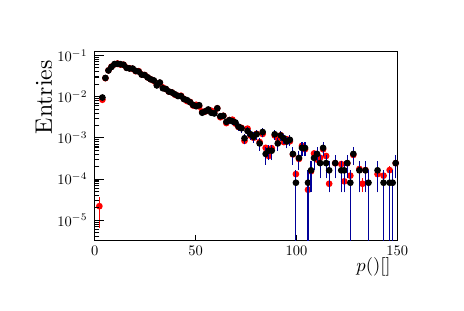
\begin{tikzpicture}
\pgfdeclareplotmark{cross} {
\pgfpathmoveto{\pgfpoint{-0.3\pgfplotmarksize}{\pgfplotmarksize}}
\pgfpathlineto{\pgfpoint{+0.3\pgfplotmarksize}{\pgfplotmarksize}}
\pgfpathlineto{\pgfpoint{+0.3\pgfplotmarksize}{0.3\pgfplotmarksize}}
\pgfpathlineto{\pgfpoint{+1\pgfplotmarksize}{0.3\pgfplotmarksize}}
\pgfpathlineto{\pgfpoint{+1\pgfplotmarksize}{-0.3\pgfplotmarksize}}
\pgfpathlineto{\pgfpoint{+0.3\pgfplotmarksize}{-0.3\pgfplotmarksize}}
\pgfpathlineto{\pgfpoint{+0.3\pgfplotmarksize}{-1.\pgfplotmarksize}}
\pgfpathlineto{\pgfpoint{-0.3\pgfplotmarksize}{-1.\pgfplotmarksize}}
\pgfpathlineto{\pgfpoint{-0.3\pgfplotmarksize}{-0.3\pgfplotmarksize}}
\pgfpathlineto{\pgfpoint{-1.\pgfplotmarksize}{-0.3\pgfplotmarksize}}
\pgfpathlineto{\pgfpoint{-1.\pgfplotmarksize}{0.3\pgfplotmarksize}}
\pgfpathlineto{\pgfpoint{-0.3\pgfplotmarksize}{0.3\pgfplotmarksize}}
\pgfpathclose
\pgfusepathqstroke
}
\pgfdeclareplotmark{cross*} {
\pgfpathmoveto{\pgfpoint{-0.3\pgfplotmarksize}{\pgfplotmarksize}}
\pgfpathlineto{\pgfpoint{+0.3\pgfplotmarksize}{\pgfplotmarksize}}
\pgfpathlineto{\pgfpoint{+0.3\pgfplotmarksize}{0.3\pgfplotmarksize}}
\pgfpathlineto{\pgfpoint{+1\pgfplotmarksize}{0.3\pgfplotmarksize}}
\pgfpathlineto{\pgfpoint{+1\pgfplotmarksize}{-0.3\pgfplotmarksize}}
\pgfpathlineto{\pgfpoint{+0.3\pgfplotmarksize}{-0.3\pgfplotmarksize}}
\pgfpathlineto{\pgfpoint{+0.3\pgfplotmarksize}{-1.\pgfplotmarksize}}
\pgfpathlineto{\pgfpoint{-0.3\pgfplotmarksize}{-1.\pgfplotmarksize}}
\pgfpathlineto{\pgfpoint{-0.3\pgfplotmarksize}{-0.3\pgfplotmarksize}}
\pgfpathlineto{\pgfpoint{-1.\pgfplotmarksize}{-0.3\pgfplotmarksize}}
\pgfpathlineto{\pgfpoint{-1.\pgfplotmarksize}{0.3\pgfplotmarksize}}
\pgfpathlineto{\pgfpoint{-0.3\pgfplotmarksize}{0.3\pgfplotmarksize}}
\pgfpathclose
\pgfusepathqfillstroke
}
\pgfdeclareplotmark{newstar} {
\pgfpathmoveto{\pgfqpoint{0pt}{\pgfplotmarksize}}
\pgfpathlineto{\pgfqpointpolar{44}{0.5\pgfplotmarksize}}
\pgfpathlineto{\pgfqpointpolar{18}{\pgfplotmarksize}}
\pgfpathlineto{\pgfqpointpolar{-20}{0.5\pgfplotmarksize}}
\pgfpathlineto{\pgfqpointpolar{-54}{\pgfplotmarksize}}
\pgfpathlineto{\pgfqpointpolar{-90}{0.5\pgfplotmarksize}}
\pgfpathlineto{\pgfqpointpolar{234}{\pgfplotmarksize}}
\pgfpathlineto{\pgfqpointpolar{198}{0.5\pgfplotmarksize}}
\pgfpathlineto{\pgfqpointpolar{162}{\pgfplotmarksize}}
\pgfpathlineto{\pgfqpointpolar{134}{0.5\pgfplotmarksize}}
\pgfpathclose
\pgfusepathqstroke
}
\pgfdeclareplotmark{newstar*} {
\pgfpathmoveto{\pgfqpoint{0pt}{\pgfplotmarksize}}
\pgfpathlineto{\pgfqpointpolar{44}{0.5\pgfplotmarksize}}
\pgfpathlineto{\pgfqpointpolar{18}{\pgfplotmarksize}}
\pgfpathlineto{\pgfqpointpolar{-20}{0.5\pgfplotmarksize}}
\pgfpathlineto{\pgfqpointpolar{-54}{\pgfplotmarksize}}
\pgfpathlineto{\pgfqpointpolar{-90}{0.5\pgfplotmarksize}}
\pgfpathlineto{\pgfqpointpolar{234}{\pgfplotmarksize}}
\pgfpathlineto{\pgfqpointpolar{198}{0.5\pgfplotmarksize}}
\pgfpathlineto{\pgfqpointpolar{162}{\pgfplotmarksize}}
\pgfpathlineto{\pgfqpointpolar{134}{0.5\pgfplotmarksize}}
\pgfpathclose
\pgfusepathqfillstroke
}
\definecolor{c}{rgb}{1,1,1};
\draw [color=c, fill=c] (5.1,0.0624161) rectangle (9.9,3.05839);
\draw [color=c, fill=c] (5.58,0.362013) rectangle (9.42,2.75879);
\definecolor{c}{rgb}{0,0,0};
\draw [c] (5.58,0.362013) -- (5.58,2.75879) -- (9.42,2.75879) -- (9.42,0.362013) -- (5.58,0.362013);
\definecolor{c}{rgb}{1,0,0};
\draw [c] (5.6376,0.519539) -- (5.6376,0.798603);
\draw [c] (5.6376,0.798603) -- (5.6376,0.920142);
\draw [c] (5.6184,0.798603) -- (5.6376,0.798603);
\draw [c] (5.6376,0.798603) -- (5.6568,0.798603);
\foreach \P in {(5.6376,0.798603)}{\draw[mark options={color=c,fill=c},mark size=2.402402pt,mark=*,mark size=1pt] plot coordinates {\P};}
\draw [c] (5.676,2.142) -- (5.676,2.15036);
\draw [c] (5.676,2.15036) -- (5.676,2.15843);
\draw [c] (5.6568,2.15036) -- (5.676,2.15036);
\draw [c] (5.676,2.15036) -- (5.6952,2.15036);
\foreach \P in {(5.676,2.15036)}{\draw[mark options={color=c,fill=c},mark size=2.402402pt,mark=*,mark size=1pt] plot coordinates {\P};}
\draw [c] (5.7144,2.41958) -- (5.7144,2.42412);
\draw [c] (5.7144,2.42412) -- (5.7144,2.42858);
\draw [c] (5.6952,2.42412) -- (5.7144,2.42412);
\draw [c] (5.7144,2.42412) -- (5.7336,2.42412);
\foreach \P in {(5.7144,2.42412)}{\draw[mark options={color=c,fill=c},mark size=2.402402pt,mark=*,mark size=1pt] plot coordinates {\P};}
\draw [c] (5.7528,2.51937) -- (5.7528,2.52302);
\draw [c] (5.7528,2.52302) -- (5.7528,2.52661);
\draw [c] (5.7336,2.52302) -- (5.7528,2.52302);
\draw [c] (5.7528,2.52302) -- (5.772,2.52302);
\foreach \P in {(5.7528,2.52302)}{\draw[mark options={color=c,fill=c},mark size=2.402402pt,mark=*,mark size=1pt] plot coordinates {\P};}
\draw [c] (5.7912,2.56767) -- (5.7912,2.57095);
\draw [c] (5.7912,2.57095) -- (5.7912,2.57418);
\draw [c] (5.772,2.57095) -- (5.7912,2.57095);
\draw [c] (5.7912,2.57095) -- (5.8104,2.57095);
\foreach \P in {(5.7912,2.57095)}{\draw[mark options={color=c,fill=c},mark size=2.402402pt,mark=*,mark size=1pt] plot coordinates {\P};}
\draw [c] (5.8296,2.59565) -- (5.8296,2.59874);
\draw [c] (5.8296,2.59874) -- (5.8296,2.60178);
\draw [c] (5.8104,2.59874) -- (5.8296,2.59874);
\draw [c] (5.8296,2.59874) -- (5.8488,2.59874);
\foreach \P in {(5.8296,2.59874)}{\draw[mark options={color=c,fill=c},mark size=2.402402pt,mark=*,mark size=1pt] plot coordinates {\P};}
\draw [c] (5.868,2.60759) -- (5.868,2.61059);
\draw [c] (5.868,2.61059) -- (5.868,2.61355);
\draw [c] (5.8488,2.61059) -- (5.868,2.61059);
\draw [c] (5.868,2.61059) -- (5.8872,2.61059);
\foreach \P in {(5.868,2.61059)}{\draw[mark options={color=c,fill=c},mark size=2.402402pt,mark=*,mark size=1pt] plot coordinates {\P};}
\draw [c] (5.9064,2.59294) -- (5.9064,2.59604);
\draw [c] (5.9064,2.59604) -- (5.9064,2.5991);
\draw [c] (5.8872,2.59604) -- (5.9064,2.59604);
\draw [c] (5.9064,2.59604) -- (5.9256,2.59604);
\foreach \P in {(5.9064,2.59604)}{\draw[mark options={color=c,fill=c},mark size=2.402402pt,mark=*,mark size=1pt] plot coordinates {\P};}
\draw [c] (5.9448,2.59167) -- (5.9448,2.59478);
\draw [c] (5.9448,2.59478) -- (5.9448,2.59785);
\draw [c] (5.9256,2.59478) -- (5.9448,2.59478);
\draw [c] (5.9448,2.59478) -- (5.964,2.59478);
\foreach \P in {(5.9448,2.59478)}{\draw[mark options={color=c,fill=c},mark size=2.402402pt,mark=*,mark size=1pt] plot coordinates {\P};}
\draw [c] (5.9832,2.55423) -- (5.9832,2.55761);
\draw [c] (5.9832,2.55761) -- (5.9832,2.56093);
\draw [c] (5.964,2.55761) -- (5.9832,2.55761);
\draw [c] (5.9832,2.55761) -- (6.0024,2.55761);
\foreach \P in {(5.9832,2.55761)}{\draw[mark options={color=c,fill=c},mark size=2.402402pt,mark=*,mark size=1pt] plot coordinates {\P};}
\draw [c] (6.0216,2.5455) -- (6.0216,2.54894);
\draw [c] (6.0216,2.54894) -- (6.0216,2.55233);
\draw [c] (6.0024,2.54894) -- (6.0216,2.54894);
\draw [c] (6.0216,2.54894) -- (6.0408,2.54894);
\foreach \P in {(6.0216,2.54894)}{\draw[mark options={color=c,fill=c},mark size=2.402402pt,mark=*,mark size=1pt] plot coordinates {\P};}
\draw [c] (6.06,2.53915) -- (6.06,2.54264);
\draw [c] (6.06,2.54264) -- (6.06,2.54608);
\draw [c] (6.0408,2.54264) -- (6.06,2.54264);
\draw [c] (6.06,2.54264) -- (6.0792,2.54264);
\foreach \P in {(6.06,2.54264)}{\draw[mark options={color=c,fill=c},mark size=2.402402pt,mark=*,mark size=1pt] plot coordinates {\P};}
\draw [c] (6.0984,2.50929) -- (6.0984,2.51302);
\draw [c] (6.0984,2.51302) -- (6.0984,2.51668);
\draw [c] (6.0792,2.51302) -- (6.0984,2.51302);
\draw [c] (6.0984,2.51302) -- (6.1176,2.51302);
\foreach \P in {(6.0984,2.51302)}{\draw[mark options={color=c,fill=c},mark size=2.402402pt,mark=*,mark size=1pt] plot coordinates {\P};}
\draw [c] (6.1368,2.50959) -- (6.1368,2.51332);
\draw [c] (6.1368,2.51332) -- (6.1368,2.51698);
\draw [c] (6.1176,2.51332) -- (6.1368,2.51332);
\draw [c] (6.1368,2.51332) -- (6.156,2.51332);
\foreach \P in {(6.1368,2.51332)}{\draw[mark options={color=c,fill=c},mark size=2.402402pt,mark=*,mark size=1pt] plot coordinates {\P};}
\draw [c] (6.1752,2.4663) -- (6.1752,2.4704);
\draw [c] (6.1752,2.4704) -- (6.1752,2.47442);
\draw [c] (6.156,2.4704) -- (6.1752,2.4704);
\draw [c] (6.1752,2.4704) -- (6.1944,2.4704);
\foreach \P in {(6.1752,2.4704)}{\draw[mark options={color=c,fill=c},mark size=2.402402pt,mark=*,mark size=1pt] plot coordinates {\P};}
\draw [c] (6.2136,2.45969) -- (6.2136,2.46385);
\draw [c] (6.2136,2.46385) -- (6.2136,2.46793);
\draw [c] (6.1944,2.46385) -- (6.2136,2.46385);
\draw [c] (6.2136,2.46385) -- (6.2328,2.46385);
\foreach \P in {(6.2136,2.46385)}{\draw[mark options={color=c,fill=c},mark size=2.402402pt,mark=*,mark size=1pt] plot coordinates {\P};}
\draw [c] (6.252,2.42831) -- (6.252,2.43276);
\draw [c] (6.252,2.43276) -- (6.252,2.43713);
\draw [c] (6.2328,2.43276) -- (6.252,2.43276);
\draw [c] (6.252,2.43276) -- (6.2712,2.43276);
\foreach \P in {(6.252,2.43276)}{\draw[mark options={color=c,fill=c},mark size=2.402402pt,mark=*,mark size=1pt] plot coordinates {\P};}
\draw [c] (6.2904,2.40483) -- (6.2904,2.40952);
\draw [c] (6.2904,2.40952) -- (6.2904,2.41412);
\draw [c] (6.2712,2.40952) -- (6.2904,2.40952);
\draw [c] (6.2904,2.40952) -- (6.3096,2.40952);
\foreach \P in {(6.2904,2.40952)}{\draw[mark options={color=c,fill=c},mark size=2.402402pt,mark=*,mark size=1pt] plot coordinates {\P};}
\draw [c] (6.3288,2.38575) -- (6.3288,2.39064);
\draw [c] (6.3288,2.39064) -- (6.3288,2.39543);
\draw [c] (6.3096,2.39064) -- (6.3288,2.39064);
\draw [c] (6.3288,2.39064) -- (6.348,2.39064);
\foreach \P in {(6.3288,2.39064)}{\draw[mark options={color=c,fill=c},mark size=2.402402pt,mark=*,mark size=1pt] plot coordinates {\P};}
\draw [c] (6.3672,2.33524) -- (6.3672,2.3407);
\draw [c] (6.3672,2.3407) -- (6.3672,2.34604);
\draw [c] (6.348,2.3407) -- (6.3672,2.3407);
\draw [c] (6.3672,2.3407) -- (6.3864,2.3407);
\foreach \P in {(6.3672,2.3407)}{\draw[mark options={color=c,fill=c},mark size=2.402402pt,mark=*,mark size=1pt] plot coordinates {\P};}
\draw [c] (6.4056,2.35868) -- (6.4056,2.36388);
\draw [c] (6.4056,2.36388) -- (6.4056,2.36895);
\draw [c] (6.3864,2.36388) -- (6.4056,2.36388);
\draw [c] (6.4056,2.36388) -- (6.4248,2.36388);
\foreach \P in {(6.4056,2.36388)}{\draw[mark options={color=c,fill=c},mark size=2.402402pt,mark=*,mark size=1pt] plot coordinates {\P};}
\draw [c] (6.444,2.30019) -- (6.444,2.3061);
\draw [c] (6.444,2.3061) -- (6.444,2.31185);
\draw [c] (6.4248,2.3061) -- (6.444,2.3061);
\draw [c] (6.444,2.3061) -- (6.4632,2.3061);
\foreach \P in {(6.444,2.3061)}{\draw[mark options={color=c,fill=c},mark size=2.402402pt,mark=*,mark size=1pt] plot coordinates {\P};}
\draw [c] (6.4824,2.27844) -- (6.4824,2.28463);
\draw [c] (6.4824,2.28463) -- (6.4824,2.29066);
\draw [c] (6.4632,2.28463) -- (6.4824,2.28463);
\draw [c] (6.4824,2.28463) -- (6.5016,2.28463);
\foreach \P in {(6.4824,2.28463)}{\draw[mark options={color=c,fill=c},mark size=2.402402pt,mark=*,mark size=1pt] plot coordinates {\P};}
\draw [c] (6.5208,2.24649) -- (6.5208,2.25313);
\draw [c] (6.5208,2.25313) -- (6.5208,2.25959);
\draw [c] (6.5016,2.25313) -- (6.5208,2.25313);
\draw [c] (6.5208,2.25313) -- (6.54,2.25313);
\foreach \P in {(6.5208,2.25313)}{\draw[mark options={color=c,fill=c},mark size=2.402402pt,mark=*,mark size=1pt] plot coordinates {\P};}
\draw [c] (6.5592,2.2361) -- (6.5592,2.2429);
\draw [c] (6.5592,2.2429) -- (6.5592,2.2495);
\draw [c] (6.54,2.2429) -- (6.5592,2.2429);
\draw [c] (6.5592,2.2429) -- (6.5784,2.2429);
\foreach \P in {(6.5592,2.2429)}{\draw[mark options={color=c,fill=c},mark size=2.402402pt,mark=*,mark size=1pt] plot coordinates {\P};}
\draw [c] (6.5976,2.20753) -- (6.5976,2.21477);
\draw [c] (6.5976,2.21477) -- (6.5976,2.22179);
\draw [c] (6.5784,2.21477) -- (6.5976,2.21477);
\draw [c] (6.5976,2.21477) -- (6.6168,2.21477);
\foreach \P in {(6.5976,2.21477)}{\draw[mark options={color=c,fill=c},mark size=2.402402pt,mark=*,mark size=1pt] plot coordinates {\P};}
\draw [c] (6.636,2.193) -- (6.636,2.20048);
\draw [c] (6.636,2.20048) -- (6.636,2.20771);
\draw [c] (6.6168,2.20048) -- (6.636,2.20048);
\draw [c] (6.636,2.20048) -- (6.6552,2.20048);
\foreach \P in {(6.636,2.20048)}{\draw[mark options={color=c,fill=c},mark size=2.402402pt,mark=*,mark size=1pt] plot coordinates {\P};}
\draw [c] (6.6744,2.19348) -- (6.6744,2.20095);
\draw [c] (6.6744,2.20095) -- (6.6744,2.20818);
\draw [c] (6.6552,2.20095) -- (6.6744,2.20095);
\draw [c] (6.6744,2.20095) -- (6.6936,2.20095);
\foreach \P in {(6.6744,2.20095)}{\draw[mark options={color=c,fill=c},mark size=2.402402pt,mark=*,mark size=1pt] plot coordinates {\P};}
\draw [c] (6.7128,2.1506) -- (6.7128,2.1588);
\draw [c] (6.7128,2.1588) -- (6.7128,2.16672);
\draw [c] (6.6936,2.1588) -- (6.7128,2.1588);
\draw [c] (6.7128,2.1588) -- (6.732,2.1588);
\foreach \P in {(6.7128,2.1588)}{\draw[mark options={color=c,fill=c},mark size=2.402402pt,mark=*,mark size=1pt] plot coordinates {\P};}
\draw [c] (6.7512,2.12441) -- (6.7512,2.13311);
\draw [c] (6.7512,2.13311) -- (6.7512,2.14148);
\draw [c] (6.732,2.13311) -- (6.7512,2.13311);
\draw [c] (6.7512,2.13311) -- (6.7704,2.13311);
\foreach \P in {(6.7512,2.13311)}{\draw[mark options={color=c,fill=c},mark size=2.402402pt,mark=*,mark size=1pt] plot coordinates {\P};}
\draw [c] (6.7896,2.11373) -- (6.7896,2.12263);
\draw [c] (6.7896,2.12263) -- (6.7896,2.13119);
\draw [c] (6.7704,2.12263) -- (6.7896,2.12263);
\draw [c] (6.7896,2.12263) -- (6.8088,2.12263);
\foreach \P in {(6.7896,2.12263)}{\draw[mark options={color=c,fill=c},mark size=2.402402pt,mark=*,mark size=1pt] plot coordinates {\P};}
\draw [c] (6.828,2.06728) -- (6.828,2.07713);
\draw [c] (6.828,2.07713) -- (6.828,2.08658);
\draw [c] (6.8088,2.07713) -- (6.828,2.07713);
\draw [c] (6.828,2.07713) -- (6.8472,2.07713);
\foreach \P in {(6.828,2.07713)}{\draw[mark options={color=c,fill=c},mark size=2.402402pt,mark=*,mark size=1pt] plot coordinates {\P};}
\draw [c] (6.8664,2.07671) -- (6.8664,2.08636);
\draw [c] (6.8664,2.08636) -- (6.8664,2.09562);
\draw [c] (6.8472,2.08636) -- (6.8664,2.08636);
\draw [c] (6.8664,2.08636) -- (6.8856,2.08636);
\foreach \P in {(6.8664,2.08636)}{\draw[mark options={color=c,fill=c},mark size=2.402402pt,mark=*,mark size=1pt] plot coordinates {\P};}
\draw [c] (6.9048,2.05436) -- (6.9048,2.0645);
\draw [c] (6.9048,2.0645) -- (6.9048,2.07421);
\draw [c] (6.8856,2.0645) -- (6.9048,2.0645);
\draw [c] (6.9048,2.0645) -- (6.924,2.0645);
\foreach \P in {(6.9048,2.0645)}{\draw[mark options={color=c,fill=c},mark size=2.402402pt,mark=*,mark size=1pt] plot coordinates {\P};}
\draw [c] (6.9432,1.98633) -- (6.9432,1.99811);
\draw [c] (6.9432,1.99811) -- (6.9432,2.00931);
\draw [c] (6.924,1.99811) -- (6.9432,1.99811);
\draw [c] (6.9432,1.99811) -- (6.9624,1.99811);
\foreach \P in {(6.9432,1.99811)}{\draw[mark options={color=c,fill=c},mark size=2.402402pt,mark=*,mark size=1pt] plot coordinates {\P};}
\draw [c] (6.9816,1.9887) -- (6.9816,2.00042);
\draw [c] (6.9816,2.00042) -- (6.9816,2.01156);
\draw [c] (6.9624,2.00042) -- (6.9816,2.00042);
\draw [c] (6.9816,2.00042) -- (7.0008,2.00042);
\foreach \P in {(6.9816,2.00042)}{\draw[mark options={color=c,fill=c},mark size=2.402402pt,mark=*,mark size=1pt] plot coordinates {\P};}
\draw [c] (7.02,2.00242) -- (7.02,2.01379);
\draw [c] (7.02,2.01379) -- (7.02,2.02462);
\draw [c] (7.0008,2.01379) -- (7.02,2.01379);
\draw [c] (7.02,2.01379) -- (7.0392,2.01379);
\foreach \P in {(7.02,2.01379)}{\draw[mark options={color=c,fill=c},mark size=2.402402pt,mark=*,mark size=1pt] plot coordinates {\P};}
\draw [c] (7.0584,1.99907) -- (7.0584,2.01052);
\draw [c] (7.0584,2.01052) -- (7.0584,2.02143);
\draw [c] (7.0392,2.01052) -- (7.0584,2.01052);
\draw [c] (7.0584,2.01052) -- (7.0776,2.01052);
\foreach \P in {(7.0584,2.01052)}{\draw[mark options={color=c,fill=c},mark size=2.402402pt,mark=*,mark size=1pt] plot coordinates {\P};}
\draw [c] (7.0968,1.97411) -- (7.0968,1.98621);
\draw [c] (7.0968,1.98621) -- (7.0968,1.9977);
\draw [c] (7.0776,1.98621) -- (7.0968,1.98621);
\draw [c] (7.0968,1.98621) -- (7.116,1.98621);
\foreach \P in {(7.0968,1.98621)}{\draw[mark options={color=c,fill=c},mark size=2.402402pt,mark=*,mark size=1pt] plot coordinates {\P};}
\draw [c] (7.1352,2.03059) -- (7.1352,2.04128);
\draw [c] (7.1352,2.04128) -- (7.1352,2.05149);
\draw [c] (7.116,2.04128) -- (7.1352,2.04128);
\draw [c] (7.1352,2.04128) -- (7.1544,2.04128);
\foreach \P in {(7.1352,2.04128)}{\draw[mark options={color=c,fill=c},mark size=2.402402pt,mark=*,mark size=1pt] plot coordinates {\P};}
\draw [c] (7.1736,1.91425) -- (7.1736,1.92805);
\draw [c] (7.1736,1.92805) -- (7.1736,1.94106);
\draw [c] (7.1544,1.92805) -- (7.1736,1.92805);
\draw [c] (7.1736,1.92805) -- (7.1928,1.92805);
\foreach \P in {(7.1736,1.92805)}{\draw[mark options={color=c,fill=c},mark size=2.402402pt,mark=*,mark size=1pt] plot coordinates {\P};}
\draw [c] (7.212,1.93299) -- (7.212,1.94624);
\draw [c] (7.212,1.94624) -- (7.212,1.95875);
\draw [c] (7.1928,1.94624) -- (7.212,1.94624);
\draw [c] (7.212,1.94624) -- (7.2312,1.94624);
\foreach \P in {(7.212,1.94624)}{\draw[mark options={color=c,fill=c},mark size=2.402402pt,mark=*,mark size=1pt] plot coordinates {\P};}
\draw [c] (7.2504,1.83776) -- (7.2504,1.85409);
\draw [c] (7.2504,1.85409) -- (7.2504,1.86933);
\draw [c] (7.2312,1.85409) -- (7.2504,1.85409);
\draw [c] (7.2504,1.85409) -- (7.2696,1.85409);
\foreach \P in {(7.2504,1.85409)}{\draw[mark options={color=c,fill=c},mark size=2.402402pt,mark=*,mark size=1pt] plot coordinates {\P};}
\draw [c] (7.2888,1.87725) -- (7.2888,1.89222);
\draw [c] (7.2888,1.89222) -- (7.2888,1.90627);
\draw [c] (7.2696,1.89222) -- (7.2888,1.89222);
\draw [c] (7.2888,1.89222) -- (7.308,1.89222);
\foreach \P in {(7.2888,1.89222)}{\draw[mark options={color=c,fill=c},mark size=2.402402pt,mark=*,mark size=1pt] plot coordinates {\P};}
\draw [c] (7.3272,1.88198) -- (7.3272,1.8968);
\draw [c] (7.3272,1.8968) -- (7.3272,1.91071);
\draw [c] (7.308,1.8968) -- (7.3272,1.8968);
\draw [c] (7.3272,1.8968) -- (7.3464,1.8968);
\foreach \P in {(7.3272,1.8968)}{\draw[mark options={color=c,fill=c},mark size=2.402402pt,mark=*,mark size=1pt] plot coordinates {\P};}
\draw [c] (7.3656,1.83086) -- (7.3656,1.84744);
\draw [c] (7.3656,1.84744) -- (7.3656,1.86289);
\draw [c] (7.3464,1.84744) -- (7.3656,1.84744);
\draw [c] (7.3656,1.84744) -- (7.3848,1.84744);
\foreach \P in {(7.3656,1.84744)}{\draw[mark options={color=c,fill=c},mark size=2.402402pt,mark=*,mark size=1pt] plot coordinates {\P};}
\draw [c] (7.404,1.78589) -- (7.404,1.8042);
\draw [c] (7.404,1.8042) -- (7.404,1.82114);
\draw [c] (7.3848,1.8042) -- (7.404,1.8042);
\draw [c] (7.404,1.8042) -- (7.4232,1.8042);
\foreach \P in {(7.404,1.8042)}{\draw[mark options={color=c,fill=c},mark size=2.402402pt,mark=*,mark size=1pt] plot coordinates {\P};}
\draw [c] (7.4424,1.77426) -- (7.4424,1.79304);
\draw [c] (7.4424,1.79304) -- (7.4424,1.81039);
\draw [c] (7.4232,1.79304) -- (7.4424,1.79304);
\draw [c] (7.4424,1.79304) -- (7.4616,1.79304);
\foreach \P in {(7.4424,1.79304)}{\draw[mark options={color=c,fill=c},mark size=2.402402pt,mark=*,mark size=1pt] plot coordinates {\P};}
\draw [c] (7.4808,1.60076) -- (7.4808,1.62826);
\draw [c] (7.4808,1.62826) -- (7.4808,1.65278);
\draw [c] (7.4616,1.62826) -- (7.4808,1.62826);
\draw [c] (7.4808,1.62826) -- (7.5,1.62826);
\foreach \P in {(7.4808,1.62826)}{\draw[mark options={color=c,fill=c},mark size=2.402402pt,mark=*,mark size=1pt] plot coordinates {\P};}
\draw [c] (7.5192,1.76359) -- (7.5192,1.78281);
\draw [c] (7.5192,1.78281) -- (7.5192,1.80053);
\draw [c] (7.5,1.78281) -- (7.5192,1.78281);
\draw [c] (7.5192,1.78281) -- (7.5384,1.78281);
\foreach \P in {(7.5192,1.78281)}{\draw[mark options={color=c,fill=c},mark size=2.402402pt,mark=*,mark size=1pt] plot coordinates {\P};}
\draw [c] (7.5576,1.6708) -- (7.5576,1.69437);
\draw [c] (7.5576,1.69437) -- (7.5576,1.71573);
\draw [c] (7.5384,1.69437) -- (7.5576,1.69437);
\draw [c] (7.5576,1.69437) -- (7.5768,1.69437);
\foreach \P in {(7.5576,1.69437)}{\draw[mark options={color=c,fill=c},mark size=2.402402pt,mark=*,mark size=1pt] plot coordinates {\P};}
\draw [c] (7.596,1.64105) -- (7.596,1.66622);
\draw [c] (7.596,1.66622) -- (7.596,1.68888);
\draw [c] (7.5768,1.66622) -- (7.596,1.66622);
\draw [c] (7.596,1.66622) -- (7.6152,1.66622);
\foreach \P in {(7.596,1.66622)}{\draw[mark options={color=c,fill=c},mark size=2.402402pt,mark=*,mark size=1pt] plot coordinates {\P};}
\draw [c] (7.6344,1.69508) -- (7.6344,1.71743);
\draw [c] (7.6344,1.71743) -- (7.6344,1.73778);
\draw [c] (7.6152,1.71743) -- (7.6344,1.71743);
\draw [c] (7.6344,1.71743) -- (7.6536,1.71743);
\foreach \P in {(7.6344,1.71743)}{\draw[mark options={color=c,fill=c},mark size=2.402402pt,mark=*,mark size=1pt] plot coordinates {\P};}
\draw [c] (7.6728,1.5845) -- (7.6728,1.613);
\draw [c] (7.6728,1.613) -- (7.6728,1.63832);
\draw [c] (7.6536,1.613) -- (7.6728,1.613);
\draw [c] (7.6728,1.613) -- (7.692,1.613);
\foreach \P in {(7.6728,1.613)}{\draw[mark options={color=c,fill=c},mark size=2.402402pt,mark=*,mark size=1pt] plot coordinates {\P};}
\draw [c] (7.7112,1.69298) -- (7.7112,1.71543);
\draw [c] (7.7112,1.71543) -- (7.7112,1.73586);
\draw [c] (7.692,1.71543) -- (7.7112,1.71543);
\draw [c] (7.7112,1.71543) -- (7.7304,1.71543);
\foreach \P in {(7.7112,1.71543)}{\draw[mark options={color=c,fill=c},mark size=2.402402pt,mark=*,mark size=1pt] plot coordinates {\P};}
\draw [c] (7.7496,1.50512) -- (7.7496,1.53904);
\draw [c] (7.7496,1.53904) -- (7.7496,1.56855);
\draw [c] (7.7304,1.53904) -- (7.7496,1.53904);
\draw [c] (7.7496,1.53904) -- (7.7688,1.53904);
\foreach \P in {(7.7496,1.53904)}{\draw[mark options={color=c,fill=c},mark size=2.402402pt,mark=*,mark size=1pt] plot coordinates {\P};}
\draw [c] (7.788,1.39223) -- (7.788,1.4357);
\draw [c] (7.788,1.4357) -- (7.788,1.47217);
\draw [c] (7.7688,1.4357) -- (7.788,1.4357);
\draw [c] (7.788,1.4357) -- (7.8072,1.4357);
\foreach \P in {(7.788,1.4357)}{\draw[mark options={color=c,fill=c},mark size=2.402402pt,mark=*,mark size=1pt] plot coordinates {\P};}
\draw [c] (7.8264,1.50034) -- (7.8264,1.53463);
\draw [c] (7.8264,1.53463) -- (7.8264,1.56441);
\draw [c] (7.8072,1.53463) -- (7.8264,1.53463);
\draw [c] (7.8264,1.53463) -- (7.8456,1.53463);
\foreach \P in {(7.8264,1.53463)}{\draw[mark options={color=c,fill=c},mark size=2.402402pt,mark=*,mark size=1pt] plot coordinates {\P};}
\draw [c] (7.8648,1.67311) -- (7.8648,1.69657);
\draw [c] (7.8648,1.69657) -- (7.8648,1.71783);
\draw [c] (7.8456,1.69657) -- (7.8648,1.69657);
\draw [c] (7.8648,1.69657) -- (7.884,1.69657);
\foreach \P in {(7.8648,1.69657)}{\draw[mark options={color=c,fill=c},mark size=2.402402pt,mark=*,mark size=1pt] plot coordinates {\P};}
\draw [c] (7.9032,1.63839) -- (7.9032,1.66371);
\draw [c] (7.9032,1.66371) -- (7.9032,1.68648);
\draw [c] (7.884,1.66371) -- (7.9032,1.66371);
\draw [c] (7.9032,1.66371) -- (7.9224,1.66371);
\foreach \P in {(7.9032,1.66371)}{\draw[mark options={color=c,fill=c},mark size=2.402402pt,mark=*,mark size=1pt] plot coordinates {\P};}
\draw [c] (7.9416,1.6754) -- (7.9416,1.69874);
\draw [c] (7.9416,1.69874) -- (7.9416,1.7199);
\draw [c] (7.9224,1.69874) -- (7.9416,1.69874);
\draw [c] (7.9416,1.69874) -- (7.9608,1.69874);
\foreach \P in {(7.9416,1.69874)}{\draw[mark options={color=c,fill=c},mark size=2.402402pt,mark=*,mark size=1pt] plot coordinates {\P};}
\draw [c] (7.98,1.5845) -- (7.98,1.613);
\draw [c] (7.98,1.613) -- (7.98,1.63832);
\draw [c] (7.9608,1.613) -- (7.98,1.613);
\draw [c] (7.98,1.613) -- (7.9992,1.613);
\foreach \P in {(7.98,1.613)}{\draw[mark options={color=c,fill=c},mark size=2.402402pt,mark=*,mark size=1pt] plot coordinates {\P};}
\draw [c] (8.0184,1.62177) -- (8.0184,1.64803);
\draw [c] (8.0184,1.64803) -- (8.0184,1.67156);
\draw [c] (7.9992,1.64803) -- (8.0184,1.64803);
\draw [c] (8.0184,1.64803) -- (8.0376,1.64803);
\foreach \P in {(8.0184,1.64803)}{\draw[mark options={color=c,fill=c},mark size=2.402402pt,mark=*,mark size=1pt] plot coordinates {\P};}
\draw [c] (8.0568,1.59439) -- (8.0568,1.62227);
\draw [c] (8.0568,1.62227) -- (8.0568,1.64711);
\draw [c] (8.0376,1.62227) -- (8.0568,1.62227);
\draw [c] (8.0568,1.62227) -- (8.076,1.62227);
\foreach \P in {(8.0568,1.62227)}{\draw[mark options={color=c,fill=c},mark size=2.402402pt,mark=*,mark size=1pt] plot coordinates {\P};}
\draw [c] (8.0952,1.41404) -- (8.0952,1.45547);
\draw [c] (8.0952,1.45547) -- (8.0952,1.4905);
\draw [c] (8.076,1.45547) -- (8.0952,1.45547);
\draw [c] (8.0952,1.45547) -- (8.1144,1.45547);
\foreach \P in {(8.0952,1.45547)}{\draw[mark options={color=c,fill=c},mark size=2.402402pt,mark=*,mark size=1pt] plot coordinates {\P};}
\draw [c] (8.1336,1.12839) -- (8.1336,1.2058);
\draw [c] (8.1336,1.2058) -- (8.1336,1.26344);
\draw [c] (8.1144,1.2058) -- (8.1336,1.2058);
\draw [c] (8.1336,1.2058) -- (8.1528,1.2058);
\foreach \P in {(8.1336,1.2058)}{\draw[mark options={color=c,fill=c},mark size=2.402402pt,mark=*,mark size=1pt] plot coordinates {\P};}
\draw [c] (8.172,1.35075) -- (8.172,1.39836);
\draw [c] (8.172,1.39836) -- (8.172,1.4377);
\draw [c] (8.1528,1.39836) -- (8.172,1.39836);
\draw [c] (8.172,1.39836) -- (8.1912,1.39836);
\foreach \P in {(8.172,1.39836)}{\draw[mark options={color=c,fill=c},mark size=2.402402pt,mark=*,mark size=1pt] plot coordinates {\P};}
\draw [c] (8.2104,1.53187) -- (8.2104,1.56386);
\draw [c] (8.2104,1.56386) -- (8.2104,1.5919);
\draw [c] (8.1912,1.56386) -- (8.2104,1.56386);
\draw [c] (8.2104,1.56386) -- (8.2296,1.56386);
\foreach \P in {(8.2104,1.56386)}{\draw[mark options={color=c,fill=c},mark size=2.402402pt,mark=*,mark size=1pt] plot coordinates {\P};}
\draw [c] (8.2488,1.48543) -- (8.2488,1.52085);
\draw [c] (8.2488,1.52085) -- (8.2488,1.55149);
\draw [c] (8.2296,1.52085) -- (8.2488,1.52085);
\draw [c] (8.2488,1.52085) -- (8.268,1.52085);
\foreach \P in {(8.2488,1.52085)}{\draw[mark options={color=c,fill=c},mark size=2.402402pt,mark=*,mark size=1pt] plot coordinates {\P};}
\draw [c] (8.2872,0.872124) -- (8.2872,1.00684);
\draw [c] (8.2872,1.00684) -- (8.2872,1.09085);
\draw [c] (8.268,1.00684) -- (8.2872,1.00684);
\draw [c] (8.2872,1.00684) -- (8.3064,1.00684);
\foreach \P in {(8.2872,1.00684)}{\draw[mark options={color=c,fill=c},mark size=2.402402pt,mark=*,mark size=1pt] plot coordinates {\P};}
\draw [c] (8.3256,1.17016) -- (8.3256,1.24083);
\draw [c] (8.3256,1.24083) -- (8.3256,1.29466);
\draw [c] (8.3064,1.24083) -- (8.3256,1.24083);
\draw [c] (8.3256,1.24083) -- (8.3448,1.24083);
\foreach \P in {(8.3256,1.24083)}{\draw[mark options={color=c,fill=c},mark size=2.402402pt,mark=*,mark size=1pt] plot coordinates {\P};}
\draw [c] (8.364,1.42753) -- (8.364,1.46776);
\draw [c] (8.364,1.46776) -- (8.364,1.50192);
\draw [c] (8.3448,1.46776) -- (8.364,1.46776);
\draw [c] (8.364,1.46776) -- (8.3832,1.46776);
\foreach \P in {(8.364,1.46776)}{\draw[mark options={color=c,fill=c},mark size=2.402402pt,mark=*,mark size=1pt] plot coordinates {\P};}
\draw [c] (8.4024,1.34152) -- (8.4024,1.39009);
\draw [c] (8.4024,1.39009) -- (8.4024,1.43009);
\draw [c] (8.3832,1.39009) -- (8.4024,1.39009);
\draw [c] (8.4024,1.39009) -- (8.4216,1.39009);
\foreach \P in {(8.4024,1.39009)}{\draw[mark options={color=c,fill=c},mark size=2.402402pt,mark=*,mark size=1pt] plot coordinates {\P};}
\draw [c] (8.4408,1.36822) -- (8.4408,1.41404);
\draw [c] (8.4408,1.41404) -- (8.4408,1.45215);
\draw [c] (8.4216,1.41404) -- (8.4408,1.41404);
\draw [c] (8.4408,1.41404) -- (8.46,1.41404);
\foreach \P in {(8.4408,1.41404)}{\draw[mark options={color=c,fill=c},mark size=2.402402pt,mark=*,mark size=1pt] plot coordinates {\P};}
\draw [c] (8.4792,1.48543) -- (8.4792,1.52085);
\draw [c] (8.4792,1.52085) -- (8.4792,1.55149);
\draw [c] (8.46,1.52085) -- (8.4792,1.52085);
\draw [c] (8.4792,1.52085) -- (8.4984,1.52085);
\foreach \P in {(8.4792,1.52085)}{\draw[mark options={color=c,fill=c},mark size=2.402402pt,mark=*,mark size=1pt] plot coordinates {\P};}
\draw [c] (8.5176,1.39223) -- (8.5176,1.4357);
\draw [c] (8.5176,1.4357) -- (8.5176,1.47217);
\draw [c] (8.4984,1.4357) -- (8.5176,1.4357);
\draw [c] (8.5176,1.4357) -- (8.5368,1.4357);
\foreach \P in {(8.5176,1.4357)}{\draw[mark options={color=c,fill=c},mark size=2.402402pt,mark=*,mark size=1pt] plot coordinates {\P};}
\draw [c] (8.556,0.975413) -- (8.556,1.08331);
\draw [c] (8.556,1.08331) -- (8.556,1.15617);
\draw [c] (8.5368,1.08331) -- (8.556,1.08331);
\draw [c] (8.556,1.08331) -- (8.5752,1.08331);
\foreach \P in {(8.556,1.08331)}{\draw[mark options={color=c,fill=c},mark size=2.402402pt,mark=*,mark size=1pt] plot coordinates {\P};}
\draw [c] (8.6328,1.28906) -- (8.6328,1.34355);
\draw [c] (8.6328,1.34355) -- (8.6328,1.38747);
\draw [c] (8.6136,1.34355) -- (8.6328,1.34355);
\draw [c] (8.6328,1.34355) -- (8.652,1.34355);
\foreach \P in {(8.6328,1.34355)}{\draw[mark options={color=c,fill=c},mark size=2.402402pt,mark=*,mark size=1pt] plot coordinates {\P};}
\draw [c] (8.7096,1.27703) -- (8.7096,1.33298);
\draw [c] (8.7096,1.33298) -- (8.7096,1.37784);
\draw [c] (8.6904,1.33298) -- (8.7096,1.33298);
\draw [c] (8.7096,1.33298) -- (8.7288,1.33298);
\foreach \P in {(8.7096,1.33298)}{\draw[mark options={color=c,fill=c},mark size=2.402402pt,mark=*,mark size=1pt] plot coordinates {\P};}
\draw [c] (8.748,1.01451) -- (8.748,1.11365);
\draw [c] (8.748,1.11365) -- (8.748,1.18245);
\draw [c] (8.7288,1.11365) -- (8.748,1.11365);
\draw [c] (8.748,1.11365) -- (8.7672,1.11365);
\foreach \P in {(8.748,1.11365)}{\draw[mark options={color=c,fill=c},mark size=2.402402pt,mark=*,mark size=1pt] plot coordinates {\P};}
\draw [c] (8.7864,1.28906) -- (8.7864,1.34355);
\draw [c] (8.7864,1.34355) -- (8.7864,1.38747);
\draw [c] (8.7672,1.34355) -- (8.7864,1.34355);
\draw [c] (8.7864,1.34355) -- (8.8056,1.34355);
\foreach \P in {(8.7864,1.34355)}{\draw[mark options={color=c,fill=c},mark size=2.402402pt,mark=*,mark size=1pt] plot coordinates {\P};}
\draw [c] (8.8248,1.10448) -- (8.8248,1.18603);
\draw [c] (8.8248,1.18603) -- (8.8248,1.24592);
\draw [c] (8.8056,1.18603) -- (8.8248,1.18603);
\draw [c] (8.8248,1.18603) -- (8.844,1.18603);
\foreach \P in {(8.8248,1.18603)}{\draw[mark options={color=c,fill=c},mark size=2.402402pt,mark=*,mark size=1pt] plot coordinates {\P};}
\draw [c] (8.8632,1.40699) -- (8.8632,1.44907);
\draw [c] (8.8632,1.44907) -- (8.8632,1.48456);
\draw [c] (8.844,1.44907) -- (8.8632,1.44907);
\draw [c] (8.8632,1.44907) -- (8.8824,1.44907);
\foreach \P in {(8.8632,1.44907)}{\draw[mark options={color=c,fill=c},mark size=2.402402pt,mark=*,mark size=1pt] plot coordinates {\P};}
\draw [c] (8.94,1.2058) -- (8.94,1.27118);
\draw [c] (8.94,1.27118) -- (8.94,1.32189);
\draw [c] (8.9208,1.27118) -- (8.94,1.27118);
\draw [c] (8.94,1.27118) -- (8.9592,1.27118);
\foreach \P in {(8.94,1.27118)}{\draw[mark options={color=c,fill=c},mark size=2.402402pt,mark=*,mark size=1pt] plot coordinates {\P};}
\draw [c] (8.9784,0.975413) -- (8.9784,1.08331);
\draw [c] (8.9784,1.08331) -- (8.9784,1.15617);
\draw [c] (8.9592,1.08331) -- (8.9784,1.08331);
\draw [c] (8.9784,1.08331) -- (8.9976,1.08331);
\foreach \P in {(8.9784,1.08331)}{\draw[mark options={color=c,fill=c},mark size=2.402402pt,mark=*,mark size=1pt] plot coordinates {\P};}
\draw [c] (9.0168,1.18863) -- (9.0168,1.25651);
\draw [c] (9.0168,1.25651) -- (9.0168,1.30871);
\draw [c] (8.9976,1.25651) -- (9.0168,1.25651);
\draw [c] (9.0168,1.25651) -- (9.036,1.25651);
\foreach \P in {(9.0168,1.25651)}{\draw[mark options={color=c,fill=c},mark size=2.402402pt,mark=*,mark size=1pt] plot coordinates {\P};}
\draw [c] (9.1704,1.12839) -- (9.1704,1.2058);
\draw [c] (9.1704,1.2058) -- (9.1704,1.26344);
\draw [c] (9.1512,1.2058) -- (9.1704,1.2058);
\draw [c] (9.1704,1.2058) -- (9.1896,1.2058);
\foreach \P in {(9.1704,1.2058)}{\draw[mark options={color=c,fill=c},mark size=2.402402pt,mark=*,mark size=1pt] plot coordinates {\P};}
\draw [c] (9.2472,1.10448) -- (9.2472,1.18603);
\draw [c] (9.2472,1.18603) -- (9.2472,1.24592);
\draw [c] (9.228,1.18603) -- (9.2472,1.18603);
\draw [c] (9.2472,1.18603) -- (9.2664,1.18603);
\foreach \P in {(9.2472,1.18603)}{\draw[mark options={color=c,fill=c},mark size=2.402402pt,mark=*,mark size=1pt] plot coordinates {\P};}
\draw [c] (9.324,1.18863) -- (9.324,1.25651);
\draw [c] (9.324,1.25651) -- (9.324,1.30871);
\draw [c] (9.3048,1.25651) -- (9.324,1.25651);
\draw [c] (9.324,1.25651) -- (9.3432,1.25651);
\foreach \P in {(9.324,1.25651)}{\draw[mark options={color=c,fill=c},mark size=2.402402pt,mark=*,mark size=1pt] plot coordinates {\P};}
\draw [c] (9.4008,1.28906) -- (9.4008,1.34355);
\draw [c] (9.4008,1.34355) -- (9.4008,1.38747);
\draw [c] (9.3816,1.34355) -- (9.4008,1.34355);
\draw [c] (9.4008,1.34355) -- (9.42,1.34355);
\foreach \P in {(9.4008,1.34355)}{\draw[mark options={color=c,fill=c},mark size=2.402402pt,mark=*,mark size=1pt] plot coordinates {\P};}
\definecolor{c}{rgb}{0,0,0};
\draw [c] (5.58,0.362013) -- (9.42,0.362013);
\draw [anchor= east] (9.42,0.0264644) node[scale=0.672873, rotate=0]{$p(\pion) [\mevc]$};
\draw [c] (5.58,0.433917) -- (5.58,0.362013);
\draw [c] (6.86,0.433917) -- (6.86,0.362013);
\draw [c] (8.14,0.433917) -- (8.14,0.362013);
\draw [c] (9.42,0.433917) -- (9.42,0.362013);
\draw [anchor=base] (5.58,0.170271) node[scale=0.523346, rotate=0]{0};
\draw [anchor=base] (6.86,0.170271) node[scale=0.523346, rotate=0]{50};
\draw [anchor=base] (8.14,0.170271) node[scale=0.523346, rotate=0]{100};
\draw [anchor=base] (9.42,0.170271) node[scale=0.523346, rotate=0]{150};
\draw [c] (5.58,0.362013) -- (5.58,2.75879);
\draw [anchor= east] (4.93104,2.75879) node[scale=0.859782, rotate=90]{Entries};
\draw [c] (5.6376,0.410896) -- (5.58,0.410896);
\draw [c] (5.6376,0.461607) -- (5.58,0.461607);
\draw [c] (5.6376,0.503042) -- (5.58,0.503042);
\draw [c] (5.6376,0.538074) -- (5.58,0.538074);
\draw [c] (5.6376,0.568421) -- (5.58,0.568421);
\draw [c] (5.6376,0.595188) -- (5.58,0.595188);
\draw [c] (5.6952,0.619133) -- (5.58,0.619133);
\draw [anchor= east] (5.54928,0.619133) node[scale=0.523346, rotate=0]{$10^{-5}$};
\draw [c] (5.6376,0.776658) -- (5.58,0.776658);
\draw [c] (5.6376,0.868804) -- (5.58,0.868804);
\draw [c] (5.6376,0.934183) -- (5.58,0.934183);
\draw [c] (5.6376,0.984895) -- (5.58,0.984895);
\draw [c] (5.6376,1.02633) -- (5.58,1.02633);
\draw [c] (5.6376,1.06136) -- (5.58,1.06136);
\draw [c] (5.6376,1.09171) -- (5.58,1.09171);
\draw [c] (5.6376,1.11848) -- (5.58,1.11848);
\draw [c] (5.6952,1.14242) -- (5.58,1.14242);
\draw [anchor= east] (5.54928,1.14242) node[scale=0.523346, rotate=0]{$10^{-4}$};
\draw [c] (5.6376,1.29995) -- (5.58,1.29995);
\draw [c] (5.6376,1.39209) -- (5.58,1.39209);
\draw [c] (5.6376,1.45747) -- (5.58,1.45747);
\draw [c] (5.6376,1.50818) -- (5.58,1.50818);
\draw [c] (5.6376,1.54962) -- (5.58,1.54962);
\draw [c] (5.6376,1.58465) -- (5.58,1.58465);
\draw [c] (5.6376,1.615) -- (5.58,1.615);
\draw [c] (5.6376,1.64176) -- (5.58,1.64176);
\draw [c] (5.6952,1.66571) -- (5.58,1.66571);
\draw [anchor= east] (5.54928,1.66571) node[scale=0.523346, rotate=0]{$10^{-3}$};
\draw [c] (5.6376,1.82323) -- (5.58,1.82323);
\draw [c] (5.6376,1.91538) -- (5.58,1.91538);
\draw [c] (5.6376,1.98076) -- (5.58,1.98076);
\draw [c] (5.6376,2.03147) -- (5.58,2.03147);
\draw [c] (5.6376,2.0729) -- (5.58,2.0729);
\draw [c] (5.6376,2.10794) -- (5.58,2.10794);
\draw [c] (5.6376,2.13828) -- (5.58,2.13828);
\draw [c] (5.6376,2.16505) -- (5.58,2.16505);
\draw [c] (5.6952,2.189) -- (5.58,2.189);
\draw [anchor= east] (5.54928,2.189) node[scale=0.523346, rotate=0]{$10^{-2}$};
\draw [c] (5.6376,2.34652) -- (5.58,2.34652);
\draw [c] (5.6376,2.43867) -- (5.58,2.43867);
\draw [c] (5.6376,2.50405) -- (5.58,2.50405);
\draw [c] (5.6376,2.55476) -- (5.58,2.55476);
\draw [c] (5.6376,2.59619) -- (5.58,2.59619);
\draw [c] (5.6376,2.63122) -- (5.58,2.63122);
\draw [c] (5.6376,2.66157) -- (5.58,2.66157);
\draw [c] (5.6376,2.68834) -- (5.58,2.68834);
\draw [c] (5.6952,2.71228) -- (5.58,2.71228);
\draw [anchor= east] (5.54928,2.71228) node[scale=0.523346, rotate=0]{$10^{-1}$};
\definecolor{c}{rgb}{0,0,0.6};
\draw [c] (5.676,2.1564) -- (5.676,2.17844);
\draw [c] (5.676,2.17844) -- (5.676,2.19854);
\draw [c] (5.6568,2.17844) -- (5.676,2.17844);
\draw [c] (5.676,2.17844) -- (5.6952,2.17844);
\definecolor{c}{rgb}{0,0,0};
\foreach \P in {(5.676,2.17844)}{\draw[mark options={color=c,fill=c},mark size=2.402402pt,mark=*,mark size=1pt] plot coordinates {\P};}
\definecolor{c}{rgb}{0,0,0.6};
\draw [c] (5.7144,2.41431) -- (5.7144,2.42682);
\draw [c] (5.7144,2.42682) -- (5.7144,2.43867);
\draw [c] (5.6952,2.42682) -- (5.7144,2.42682);
\draw [c] (5.7144,2.42682) -- (5.7336,2.42682);
\definecolor{c}{rgb}{0,0,0};
\foreach \P in {(5.7144,2.42682)}{\draw[mark options={color=c,fill=c},mark size=2.402402pt,mark=*,mark size=1pt] plot coordinates {\P};}
\definecolor{c}{rgb}{0,0,0.6};
\draw [c] (5.7528,2.51168) -- (5.7528,2.52177);
\draw [c] (5.7528,2.52177) -- (5.7528,2.53143);
\draw [c] (5.7336,2.52177) -- (5.7528,2.52177);
\draw [c] (5.7528,2.52177) -- (5.772,2.52177);
\definecolor{c}{rgb}{0,0,0};
\foreach \P in {(5.7528,2.52177)}{\draw[mark options={color=c,fill=c},mark size=2.402402pt,mark=*,mark size=1pt] plot coordinates {\P};}
\definecolor{c}{rgb}{0,0,0.6};
\draw [c] (5.7912,2.55763) -- (5.7912,2.56675);
\draw [c] (5.7912,2.56675) -- (5.7912,2.57552);
\draw [c] (5.772,2.56675) -- (5.7912,2.56675);
\draw [c] (5.7912,2.56675) -- (5.8104,2.56675);
\definecolor{c}{rgb}{0,0,0};
\foreach \P in {(5.7912,2.56675)}{\draw[mark options={color=c,fill=c},mark size=2.402402pt,mark=*,mark size=1pt] plot coordinates {\P};}
\definecolor{c}{rgb}{0,0,0.6};
\draw [c] (5.8296,2.59437) -- (5.8296,2.60278);
\draw [c] (5.8296,2.60278) -- (5.8296,2.6109);
\draw [c] (5.8104,2.60278) -- (5.8296,2.60278);
\draw [c] (5.8296,2.60278) -- (5.8488,2.60278);
\definecolor{c}{rgb}{0,0,0};
\foreach \P in {(5.8296,2.60278)}{\draw[mark options={color=c,fill=c},mark size=2.402402pt,mark=*,mark size=1pt] plot coordinates {\P};}
\definecolor{c}{rgb}{0,0,0.6};
\draw [c] (5.868,2.59861) -- (5.868,2.60695);
\draw [c] (5.868,2.60695) -- (5.868,2.61499);
\draw [c] (5.8488,2.60695) -- (5.868,2.60695);
\draw [c] (5.868,2.60695) -- (5.8872,2.60695);
\definecolor{c}{rgb}{0,0,0};
\foreach \P in {(5.868,2.60695)}{\draw[mark options={color=c,fill=c},mark size=2.402402pt,mark=*,mark size=1pt] plot coordinates {\P};}
\definecolor{c}{rgb}{0,0,0.6};
\draw [c] (5.9064,2.59345) -- (5.9064,2.60188);
\draw [c] (5.9064,2.60188) -- (5.9064,2.61001);
\draw [c] (5.8872,2.60188) -- (5.9064,2.60188);
\draw [c] (5.9064,2.60188) -- (5.9256,2.60188);
\definecolor{c}{rgb}{0,0,0};
\foreach \P in {(5.9064,2.60188)}{\draw[mark options={color=c,fill=c},mark size=2.402402pt,mark=*,mark size=1pt] plot coordinates {\P};}
\definecolor{c}{rgb}{0,0,0.6};
\draw [c] (5.9448,2.58532) -- (5.9448,2.59391);
\draw [c] (5.9448,2.59391) -- (5.9448,2.60218);
\draw [c] (5.9256,2.59391) -- (5.9448,2.59391);
\draw [c] (5.9448,2.59391) -- (5.964,2.59391);
\definecolor{c}{rgb}{0,0,0};
\foreach \P in {(5.9448,2.59391)}{\draw[mark options={color=c,fill=c},mark size=2.402402pt,mark=*,mark size=1pt] plot coordinates {\P};}
\definecolor{c}{rgb}{0,0,0.6};
\draw [c] (5.9832,2.54584) -- (5.9832,2.5552);
\draw [c] (5.9832,2.5552) -- (5.9832,2.56419);
\draw [c] (5.964,2.5552) -- (5.9832,2.5552);
\draw [c] (5.9832,2.5552) -- (6.0024,2.5552);
\definecolor{c}{rgb}{0,0,0};
\foreach \P in {(5.9832,2.5552)}{\draw[mark options={color=c,fill=c},mark size=2.402402pt,mark=*,mark size=1pt] plot coordinates {\P};}
\definecolor{c}{rgb}{0,0,0.6};
\draw [c] (6.0216,2.53737) -- (6.0216,2.54691);
\draw [c] (6.0216,2.54691) -- (6.0216,2.55606);
\draw [c] (6.0024,2.54691) -- (6.0216,2.54691);
\draw [c] (6.0216,2.54691) -- (6.0408,2.54691);
\definecolor{c}{rgb}{0,0,0};
\foreach \P in {(6.0216,2.54691)}{\draw[mark options={color=c,fill=c},mark size=2.402402pt,mark=*,mark size=1pt] plot coordinates {\P};}
\definecolor{c}{rgb}{0,0,0.6};
\draw [c] (6.06,2.53659) -- (6.06,2.54614);
\draw [c] (6.06,2.54614) -- (6.06,2.55531);
\draw [c] (6.0408,2.54614) -- (6.06,2.54614);
\draw [c] (6.06,2.54614) -- (6.0792,2.54614);
\definecolor{c}{rgb}{0,0,0};
\foreach \P in {(6.06,2.54614)}{\draw[mark options={color=c,fill=c},mark size=2.402402pt,mark=*,mark size=1pt] plot coordinates {\P};}
\definecolor{c}{rgb}{0,0,0.6};
\draw [c] (6.0984,2.50635) -- (6.0984,2.51656);
\draw [c] (6.0984,2.51656) -- (6.0984,2.52634);
\draw [c] (6.0792,2.51656) -- (6.0984,2.51656);
\draw [c] (6.0984,2.51656) -- (6.1176,2.51656);
\definecolor{c}{rgb}{0,0,0};
\foreach \P in {(6.0984,2.51656)}{\draw[mark options={color=c,fill=c},mark size=2.402402pt,mark=*,mark size=1pt] plot coordinates {\P};}
\definecolor{c}{rgb}{0,0,0.6};
\draw [c] (6.1368,2.4972) -- (6.1368,2.50762);
\draw [c] (6.1368,2.50762) -- (6.1368,2.51758);
\draw [c] (6.1176,2.50762) -- (6.1368,2.50762);
\draw [c] (6.1368,2.50762) -- (6.156,2.50762);
\definecolor{c}{rgb}{0,0,0};
\foreach \P in {(6.1368,2.50762)}{\draw[mark options={color=c,fill=c},mark size=2.402402pt,mark=*,mark size=1pt] plot coordinates {\P};}
\definecolor{c}{rgb}{0,0,0.6};
\draw [c] (6.1752,2.45809) -- (6.1752,2.46944);
\draw [c] (6.1752,2.46944) -- (6.1752,2.48026);
\draw [c] (6.156,2.46944) -- (6.1752,2.46944);
\draw [c] (6.1752,2.46944) -- (6.1944,2.46944);
\definecolor{c}{rgb}{0,0,0};
\foreach \P in {(6.1752,2.46944)}{\draw[mark options={color=c,fill=c},mark size=2.402402pt,mark=*,mark size=1pt] plot coordinates {\P};}
\definecolor{c}{rgb}{0,0,0.6};
\draw [c] (6.2136,2.45135) -- (6.2136,2.46287);
\draw [c] (6.2136,2.46287) -- (6.2136,2.47384);
\draw [c] (6.1944,2.46287) -- (6.2136,2.46287);
\draw [c] (6.2136,2.46287) -- (6.2328,2.46287);
\definecolor{c}{rgb}{0,0,0};
\foreach \P in {(6.2136,2.46287)}{\draw[mark options={color=c,fill=c},mark size=2.402402pt,mark=*,mark size=1pt] plot coordinates {\P};}
\definecolor{c}{rgb}{0,0,0.6};
\draw [c] (6.252,2.42092) -- (6.252,2.43324);
\draw [c] (6.252,2.43324) -- (6.252,2.44493);
\draw [c] (6.2328,2.43324) -- (6.252,2.43324);
\draw [c] (6.252,2.43324) -- (6.2712,2.43324);
\definecolor{c}{rgb}{0,0,0};
\foreach \P in {(6.252,2.43324)}{\draw[mark options={color=c,fill=c},mark size=2.402402pt,mark=*,mark size=1pt] plot coordinates {\P};}
\definecolor{c}{rgb}{0,0,0.6};
\draw [c] (6.2904,2.39621) -- (6.2904,2.40922);
\draw [c] (6.2904,2.40922) -- (6.2904,2.42153);
\draw [c] (6.2712,2.40922) -- (6.2904,2.40922);
\draw [c] (6.2904,2.40922) -- (6.3096,2.40922);
\definecolor{c}{rgb}{0,0,0};
\foreach \P in {(6.2904,2.40922)}{\draw[mark options={color=c,fill=c},mark size=2.402402pt,mark=*,mark size=1pt] plot coordinates {\P};}
\definecolor{c}{rgb}{0,0,0.6};
\draw [c] (6.3288,2.38202) -- (6.3288,2.39545);
\draw [c] (6.3288,2.39545) -- (6.3288,2.40812);
\draw [c] (6.3096,2.39545) -- (6.3288,2.39545);
\draw [c] (6.3288,2.39545) -- (6.348,2.39545);
\definecolor{c}{rgb}{0,0,0};
\foreach \P in {(6.3288,2.39545)}{\draw[mark options={color=c,fill=c},mark size=2.402402pt,mark=*,mark size=1pt] plot coordinates {\P};}
\definecolor{c}{rgb}{0,0,0.6};
\draw [c] (6.3672,2.31655) -- (6.3672,2.33205);
\draw [c] (6.3672,2.33205) -- (6.3672,2.34656);
\draw [c] (6.348,2.33205) -- (6.3672,2.33205);
\draw [c] (6.3672,2.33205) -- (6.3864,2.33205);
\definecolor{c}{rgb}{0,0,0};
\foreach \P in {(6.3672,2.33205)}{\draw[mark options={color=c,fill=c},mark size=2.402402pt,mark=*,mark size=1pt] plot coordinates {\P};}
\definecolor{c}{rgb}{0,0,0.6};
\draw [c] (6.4056,2.35422) -- (6.4056,2.36849);
\draw [c] (6.4056,2.36849) -- (6.4056,2.38192);
\draw [c] (6.3864,2.36849) -- (6.4056,2.36849);
\draw [c] (6.4056,2.36849) -- (6.4248,2.36849);
\definecolor{c}{rgb}{0,0,0};
\foreach \P in {(6.4056,2.36849)}{\draw[mark options={color=c,fill=c},mark size=2.402402pt,mark=*,mark size=1pt] plot coordinates {\P};}
\definecolor{c}{rgb}{0,0,0.6};
\draw [c] (6.444,2.27886) -- (6.444,2.2957);
\draw [c] (6.444,2.2957) -- (6.444,2.31138);
\draw [c] (6.4248,2.2957) -- (6.444,2.2957);
\draw [c] (6.444,2.2957) -- (6.4632,2.2957);
\definecolor{c}{rgb}{0,0,0};
\foreach \P in {(6.444,2.2957)}{\draw[mark options={color=c,fill=c},mark size=2.402402pt,mark=*,mark size=1pt] plot coordinates {\P};}
\definecolor{c}{rgb}{0,0,0.6};
\draw [c] (6.4824,2.26902) -- (6.4824,2.28623);
\draw [c] (6.4824,2.28623) -- (6.4824,2.30223);
\draw [c] (6.4632,2.28623) -- (6.4824,2.28623);
\draw [c] (6.4824,2.28623) -- (6.5016,2.28623);
\definecolor{c}{rgb}{0,0,0};
\foreach \P in {(6.4824,2.28623)}{\draw[mark options={color=c,fill=c},mark size=2.402402pt,mark=*,mark size=1pt] plot coordinates {\P};}
\definecolor{c}{rgb}{0,0,0.6};
\draw [c] (6.5208,2.23526) -- (6.5208,2.2538);
\draw [c] (6.5208,2.2538) -- (6.5208,2.27094);
\draw [c] (6.5016,2.2538) -- (6.5208,2.2538);
\draw [c] (6.5208,2.2538) -- (6.54,2.2538);
\definecolor{c}{rgb}{0,0,0};
\foreach \P in {(6.5208,2.2538)}{\draw[mark options={color=c,fill=c},mark size=2.402402pt,mark=*,mark size=1pt] plot coordinates {\P};}
\definecolor{c}{rgb}{0,0,0.6};
\draw [c] (6.5592,2.22333) -- (6.5592,2.24236);
\draw [c] (6.5592,2.24236) -- (6.5592,2.25992);
\draw [c] (6.54,2.24236) -- (6.5592,2.24236);
\draw [c] (6.5592,2.24236) -- (6.5784,2.24236);
\definecolor{c}{rgb}{0,0,0};
\foreach \P in {(6.5592,2.24236)}{\draw[mark options={color=c,fill=c},mark size=2.402402pt,mark=*,mark size=1pt] plot coordinates {\P};}
\definecolor{c}{rgb}{0,0,0.6};
\draw [c] (6.5976,2.19916) -- (6.5976,2.21923);
\draw [c] (6.5976,2.21923) -- (6.5976,2.23767);
\draw [c] (6.5784,2.21923) -- (6.5976,2.21923);
\draw [c] (6.5976,2.21923) -- (6.6168,2.21923);
\definecolor{c}{rgb}{0,0,0};
\foreach \P in {(6.5976,2.21923)}{\draw[mark options={color=c,fill=c},mark size=2.402402pt,mark=*,mark size=1pt] plot coordinates {\P};}
\definecolor{c}{rgb}{0,0,0.6};
\draw [c] (6.636,2.17597) -- (6.636,2.19708);
\draw [c] (6.636,2.19708) -- (6.636,2.2164);
\draw [c] (6.6168,2.19708) -- (6.636,2.19708);
\draw [c] (6.636,2.19708) -- (6.6552,2.19708);
\definecolor{c}{rgb}{0,0,0};
\foreach \P in {(6.636,2.19708)}{\draw[mark options={color=c,fill=c},mark size=2.402402pt,mark=*,mark size=1pt] plot coordinates {\P};}
\definecolor{c}{rgb}{0,0,0.6};
\draw [c] (6.6744,2.17408) -- (6.6744,2.19529);
\draw [c] (6.6744,2.19529) -- (6.6744,2.21468);
\draw [c] (6.6552,2.19529) -- (6.6744,2.19529);
\draw [c] (6.6744,2.19529) -- (6.6936,2.19529);
\definecolor{c}{rgb}{0,0,0};
\foreach \P in {(6.6744,2.19529)}{\draw[mark options={color=c,fill=c},mark size=2.402402pt,mark=*,mark size=1pt] plot coordinates {\P};}
\definecolor{c}{rgb}{0,0,0.6};
\draw [c] (6.7128,2.13503) -- (6.7128,2.15814);
\draw [c] (6.7128,2.15814) -- (6.7128,2.17911);
\draw [c] (6.6936,2.15814) -- (6.7128,2.15814);
\draw [c] (6.7128,2.15814) -- (6.732,2.15814);
\definecolor{c}{rgb}{0,0,0};
\foreach \P in {(6.7128,2.15814)}{\draw[mark options={color=c,fill=c},mark size=2.402402pt,mark=*,mark size=1pt] plot coordinates {\P};}
\definecolor{c}{rgb}{0,0,0.6};
\draw [c] (6.7512,2.12121) -- (6.7512,2.14503);
\draw [c] (6.7512,2.14503) -- (6.7512,2.16658);
\draw [c] (6.732,2.14503) -- (6.7512,2.14503);
\draw [c] (6.7512,2.14503) -- (6.7704,2.14503);
\definecolor{c}{rgb}{0,0,0};
\foreach \P in {(6.7512,2.14503)}{\draw[mark options={color=c,fill=c},mark size=2.402402pt,mark=*,mark size=1pt] plot coordinates {\P};}
\definecolor{c}{rgb}{0,0,0.6};
\draw [c] (6.7896,2.0935) -- (6.7896,2.11882);
\draw [c] (6.7896,2.11882) -- (6.7896,2.14159);
\draw [c] (6.7704,2.11882) -- (6.7896,2.11882);
\draw [c] (6.7896,2.11882) -- (6.8088,2.11882);
\definecolor{c}{rgb}{0,0,0};
\foreach \P in {(6.7896,2.11882)}{\draw[mark options={color=c,fill=c},mark size=2.402402pt,mark=*,mark size=1pt] plot coordinates {\P};}
\definecolor{c}{rgb}{0,0,0.6};
\draw [c] (6.828,2.05587) -- (6.828,2.08337);
\draw [c] (6.828,2.08337) -- (6.828,2.10789);
\draw [c] (6.8088,2.08337) -- (6.828,2.08337);
\draw [c] (6.828,2.08337) -- (6.8472,2.08337);
\definecolor{c}{rgb}{0,0,0};
\foreach \P in {(6.828,2.08337)}{\draw[mark options={color=c,fill=c},mark size=2.402402pt,mark=*,mark size=1pt] plot coordinates {\P};}
\definecolor{c}{rgb}{0,0,0.6};
\draw [c] (6.8664,2.03961) -- (6.8664,2.06811);
\draw [c] (6.8664,2.06811) -- (6.8664,2.09343);
\draw [c] (6.8472,2.06811) -- (6.8664,2.06811);
\draw [c] (6.8664,2.06811) -- (6.8856,2.06811);
\definecolor{c}{rgb}{0,0,0};
\foreach \P in {(6.8664,2.06811)}{\draw[mark options={color=c,fill=c},mark size=2.402402pt,mark=*,mark size=1pt] plot coordinates {\P};}
\definecolor{c}{rgb}{0,0,0.6};
\draw [c] (6.9048,2.05271) -- (6.9048,2.08039);
\draw [c] (6.9048,2.08039) -- (6.9048,2.10507);
\draw [c] (6.8856,2.08039) -- (6.9048,2.08039);
\draw [c] (6.9048,2.08039) -- (6.924,2.08039);
\definecolor{c}{rgb}{0,0,0};
\foreach \P in {(6.9048,2.08039)}{\draw[mark options={color=c,fill=c},mark size=2.402402pt,mark=*,mark size=1pt] plot coordinates {\P};}
\definecolor{c}{rgb}{0,0,0.6};
\draw [c] (6.9432,1.95059) -- (6.9432,1.98524);
\draw [c] (6.9432,1.98524) -- (6.9432,2.0153);
\draw [c] (6.924,1.98524) -- (6.9432,1.98524);
\draw [c] (6.9432,1.98524) -- (6.9624,1.98524);
\definecolor{c}{rgb}{0,0,0};
\foreach \P in {(6.9432,1.98524)}{\draw[mark options={color=c,fill=c},mark size=2.402402pt,mark=*,mark size=1pt] plot coordinates {\P};}
\definecolor{c}{rgb}{0,0,0.6};
\draw [c] (6.9816,1.96949) -- (6.9816,2.00273);
\draw [c] (6.9816,2.00273) -- (6.9816,2.03172);
\draw [c] (6.9624,2.00273) -- (6.9816,2.00273);
\draw [c] (6.9816,2.00273) -- (7.0008,2.00273);
\definecolor{c}{rgb}{0,0,0};
\foreach \P in {(6.9816,2.00273)}{\draw[mark options={color=c,fill=c},mark size=2.402402pt,mark=*,mark size=1pt] plot coordinates {\P};}
\definecolor{c}{rgb}{0,0,0.6};
\draw [c] (7.02,1.99526) -- (7.02,2.02667);
\draw [c] (7.02,2.02667) -- (7.02,2.05427);
\draw [c] (7.0008,2.02667) -- (7.02,2.02667);
\draw [c] (7.02,2.02667) -- (7.0392,2.02667);
\definecolor{c}{rgb}{0,0,0};
\foreach \P in {(7.02,2.02667)}{\draw[mark options={color=c,fill=c},mark size=2.402402pt,mark=*,mark size=1pt] plot coordinates {\P};}
\definecolor{c}{rgb}{0,0,0.6};
\draw [c] (7.0584,1.95059) -- (7.0584,1.98524);
\draw [c] (7.0584,1.98524) -- (7.0584,2.0153);
\draw [c] (7.0392,1.98524) -- (7.0584,1.98524);
\draw [c] (7.0584,1.98524) -- (7.0776,1.98524);
\definecolor{c}{rgb}{0,0,0};
\foreach \P in {(7.0584,1.98524)}{\draw[mark options={color=c,fill=c},mark size=2.402402pt,mark=*,mark size=1pt] plot coordinates {\P};}
\definecolor{c}{rgb}{0,0,0.6};
\draw [c] (7.0968,1.94054) -- (7.0968,1.97596);
\draw [c] (7.0968,1.97596) -- (7.0968,2.0066);
\draw [c] (7.0776,1.97596) -- (7.0968,1.97596);
\draw [c] (7.0968,1.97596) -- (7.116,1.97596);
\definecolor{c}{rgb}{0,0,0};
\foreach \P in {(7.0968,1.97596)}{\draw[mark options={color=c,fill=c},mark size=2.402402pt,mark=*,mark size=1pt] plot coordinates {\P};}
\definecolor{c}{rgb}{0,0,0.6};
\draw [c] (7.1352,2.01099) -- (7.1352,2.04134);
\draw [c] (7.1352,2.04134) -- (7.1352,2.06811);
\draw [c] (7.116,2.04134) -- (7.1352,2.04134);
\draw [c] (7.1352,2.04134) -- (7.1544,2.04134);
\definecolor{c}{rgb}{0,0,0};
\foreach \P in {(7.1352,2.04134)}{\draw[mark options={color=c,fill=c},mark size=2.402402pt,mark=*,mark size=1pt] plot coordinates {\P};}
\definecolor{c}{rgb}{0,0,0.6};
\draw [c] (7.1736,1.90155) -- (7.1736,1.94014);
\draw [c] (7.1736,1.94014) -- (7.1736,1.97312);
\draw [c] (7.1544,1.94014) -- (7.1736,1.94014);
\draw [c] (7.1736,1.94014) -- (7.1928,1.94014);
\definecolor{c}{rgb}{0,0,0};
\foreach \P in {(7.1736,1.94014)}{\draw[mark options={color=c,fill=c},mark size=2.402402pt,mark=*,mark size=1pt] plot coordinates {\P};}
\definecolor{c}{rgb}{0,0,0.6};
\draw [c] (7.212,1.90753) -- (7.212,1.94561);
\draw [c] (7.212,1.94561) -- (7.212,1.97823);
\draw [c] (7.1928,1.94561) -- (7.212,1.94561);
\draw [c] (7.212,1.94561) -- (7.2312,1.94561);
\definecolor{c}{rgb}{0,0,0};
\foreach \P in {(7.212,1.94561)}{\draw[mark options={color=c,fill=c},mark size=2.402402pt,mark=*,mark size=1pt] plot coordinates {\P};}
\definecolor{c}{rgb}{0,0,0.6};
\draw [c] (7.2504,1.82333) -- (7.2504,1.86915);
\draw [c] (7.2504,1.86915) -- (7.2504,1.90726);
\draw [c] (7.2312,1.86915) -- (7.2504,1.86915);
\draw [c] (7.2504,1.86915) -- (7.2696,1.86915);
\definecolor{c}{rgb}{0,0,0};
\foreach \P in {(7.2504,1.86915)}{\draw[mark options={color=c,fill=c},mark size=2.402402pt,mark=*,mark size=1pt] plot coordinates {\P};}
\definecolor{c}{rgb}{0,0,0.6};
\draw [c] (7.2888,1.84734) -- (7.2888,1.89081);
\draw [c] (7.2888,1.89081) -- (7.2888,1.92728);
\draw [c] (7.2696,1.89081) -- (7.2888,1.89081);
\draw [c] (7.2888,1.89081) -- (7.308,1.89081);
\definecolor{c}{rgb}{0,0,0};
\foreach \P in {(7.2888,1.89081)}{\draw[mark options={color=c,fill=c},mark size=2.402402pt,mark=*,mark size=1pt] plot coordinates {\P};}
\definecolor{c}{rgb}{0,0,0.6};
\draw [c] (7.3272,1.83161) -- (7.3272,1.8766);
\draw [c] (7.3272,1.8766) -- (7.3272,1.91414);
\draw [c] (7.308,1.8766) -- (7.3272,1.8766);
\draw [c] (7.3272,1.8766) -- (7.3464,1.8766);
\definecolor{c}{rgb}{0,0,0};
\foreach \P in {(7.3272,1.8766)}{\draw[mark options={color=c,fill=c},mark size=2.402402pt,mark=*,mark size=1pt] plot coordinates {\P};}
\definecolor{c}{rgb}{0,0,0.6};
\draw [c] (7.3656,1.81476) -- (7.3656,1.86144);
\draw [c] (7.3656,1.86144) -- (7.3656,1.90015);
\draw [c] (7.3464,1.86144) -- (7.3656,1.86144);
\draw [c] (7.3656,1.86144) -- (7.3848,1.86144);
\definecolor{c}{rgb}{0,0,0};
\foreach \P in {(7.3656,1.86144)}{\draw[mark options={color=c,fill=c},mark size=2.402402pt,mark=*,mark size=1pt] plot coordinates {\P};}
\definecolor{c}{rgb}{0,0,0.6};
\draw [c] (7.404,1.75562) -- (7.404,1.80876);
\draw [c] (7.404,1.80876) -- (7.404,1.8518);
\draw [c] (7.3848,1.80876) -- (7.404,1.80876);
\draw [c] (7.404,1.80876) -- (7.4232,1.80876);
\definecolor{c}{rgb}{0,0,0};
\foreach \P in {(7.404,1.80876)}{\draw[mark options={color=c,fill=c},mark size=2.402402pt,mark=*,mark size=1pt] plot coordinates {\P};}
\definecolor{c}{rgb}{0,0,0.6};
\draw [c] (7.4424,1.73214) -- (7.4424,1.78809);
\draw [c] (7.4424,1.78809) -- (7.4424,1.83295);
\draw [c] (7.4232,1.78809) -- (7.4424,1.78809);
\draw [c] (7.4424,1.78809) -- (7.4616,1.78809);
\definecolor{c}{rgb}{0,0,0};
\foreach \P in {(7.4424,1.78809)}{\draw[mark options={color=c,fill=c},mark size=2.402402pt,mark=*,mark size=1pt] plot coordinates {\P};}
\definecolor{c}{rgb}{0,0,0.6};
\draw [c] (7.4808,1.5835) -- (7.4808,1.66091);
\draw [c] (7.4808,1.66091) -- (7.4808,1.71855);
\draw [c] (7.4616,1.66091) -- (7.4808,1.66091);
\draw [c] (7.4808,1.66091) -- (7.5,1.66091);
\definecolor{c}{rgb}{0,0,0};
\foreach \P in {(7.4808,1.66091)}{\draw[mark options={color=c,fill=c},mark size=2.402402pt,mark=*,mark size=1pt] plot coordinates {\P};}
\definecolor{c}{rgb}{0,0,0.6};
\draw [c] (7.5192,1.69197) -- (7.5192,1.75306);
\draw [c] (7.5192,1.75306) -- (7.5192,1.80115);
\draw [c] (7.5,1.75306) -- (7.5192,1.75306);
\draw [c] (7.5192,1.75306) -- (7.5384,1.75306);
\definecolor{c}{rgb}{0,0,0};
\foreach \P in {(7.5192,1.75306)}{\draw[mark options={color=c,fill=c},mark size=2.402402pt,mark=*,mark size=1pt] plot coordinates {\P};}
\definecolor{c}{rgb}{0,0,0.6};
\draw [c] (7.5576,1.64375) -- (7.5576,1.71162);
\draw [c] (7.5576,1.71162) -- (7.5576,1.76382);
\draw [c] (7.5384,1.71162) -- (7.5576,1.71162);
\draw [c] (7.5576,1.71162) -- (7.5768,1.71162);
\definecolor{c}{rgb}{0,0,0};
\foreach \P in {(7.5576,1.71162)}{\draw[mark options={color=c,fill=c},mark size=2.402402pt,mark=*,mark size=1pt] plot coordinates {\P};}
\definecolor{c}{rgb}{0,0,0.6};
\draw [c] (7.596,1.60528) -- (7.596,1.6791);
\draw [c] (7.596,1.6791) -- (7.596,1.73473);
\draw [c] (7.5768,1.6791) -- (7.596,1.6791);
\draw [c] (7.596,1.6791) -- (7.6152,1.6791);
\definecolor{c}{rgb}{0,0,0};
\foreach \P in {(7.596,1.6791)}{\draw[mark options={color=c,fill=c},mark size=2.402402pt,mark=*,mark size=1pt] plot coordinates {\P};}
\definecolor{c}{rgb}{0,0,0.6};
\draw [c] (7.6344,1.64375) -- (7.6344,1.71162);
\draw [c] (7.6344,1.71162) -- (7.6344,1.76382);
\draw [c] (7.6152,1.71162) -- (7.6344,1.71162);
\draw [c] (7.6344,1.71162) -- (7.6536,1.71162);
\definecolor{c}{rgb}{0,0,0};
\foreach \P in {(7.6344,1.71162)}{\draw[mark options={color=c,fill=c},mark size=2.402402pt,mark=*,mark size=1pt] plot coordinates {\P};}
\definecolor{c}{rgb}{0,0,0.6};
\draw [c] (7.6728,1.50339) -- (7.6728,1.59553);
\draw [c] (7.6728,1.59553) -- (7.6728,1.66091);
\draw [c] (7.6536,1.59553) -- (7.6728,1.59553);
\draw [c] (7.6728,1.59553) -- (7.692,1.59553);
\definecolor{c}{rgb}{0,0,0};
\foreach \P in {(7.6728,1.59553)}{\draw[mark options={color=c,fill=c},mark size=2.402402pt,mark=*,mark size=1pt] plot coordinates {\P};}
\definecolor{c}{rgb}{0,0,0.6};
\draw [c] (7.7112,1.67694) -- (7.7112,1.74007);
\draw [c] (7.7112,1.74007) -- (7.7112,1.78942);
\draw [c] (7.692,1.74007) -- (7.7112,1.74007);
\draw [c] (7.7112,1.74007) -- (7.7304,1.74007);
\definecolor{c}{rgb}{0,0,0};
\foreach \P in {(7.7112,1.74007)}{\draw[mark options={color=c,fill=c},mark size=2.402402pt,mark=*,mark size=1pt] plot coordinates {\P};}
\definecolor{c}{rgb}{0,0,0.6};
\draw [c] (7.7496,1.32723) -- (7.7496,1.46195);
\draw [c] (7.7496,1.46195) -- (7.7496,1.54596);
\draw [c] (7.7304,1.46195) -- (7.7496,1.46195);
\draw [c] (7.7496,1.46195) -- (7.7688,1.46195);
\definecolor{c}{rgb}{0,0,0};
\foreach \P in {(7.7496,1.46195)}{\draw[mark options={color=c,fill=c},mark size=2.402402pt,mark=*,mark size=1pt] plot coordinates {\P};}
\definecolor{c}{rgb}{0,0,0.6};
\draw [c] (7.788,1.38415) -- (7.788,1.50339);
\draw [c] (7.788,1.50339) -- (7.788,1.58119);
\draw [c] (7.7688,1.50339) -- (7.788,1.50339);
\draw [c] (7.788,1.50339) -- (7.8072,1.50339);
\definecolor{c}{rgb}{0,0,0};
\foreach \P in {(7.788,1.50339)}{\draw[mark options={color=c,fill=c},mark size=2.402402pt,mark=*,mark size=1pt] plot coordinates {\P};}
\definecolor{c}{rgb}{0,0,0.6};
\draw [c] (7.8264,1.38415) -- (7.8264,1.50339);
\draw [c] (7.8264,1.50339) -- (7.8264,1.58119);
\draw [c] (7.8072,1.50339) -- (7.8264,1.50339);
\draw [c] (7.8264,1.50339) -- (7.8456,1.50339);
\definecolor{c}{rgb}{0,0,0};
\foreach \P in {(7.8264,1.50339)}{\draw[mark options={color=c,fill=c},mark size=2.402402pt,mark=*,mark size=1pt] plot coordinates {\P};}
\definecolor{c}{rgb}{0,0,0.6};
\draw [c] (7.8648,1.64375) -- (7.8648,1.71162);
\draw [c] (7.8648,1.71162) -- (7.8648,1.76382);
\draw [c] (7.8456,1.71162) -- (7.8648,1.71162);
\draw [c] (7.8648,1.71162) -- (7.884,1.71162);
\definecolor{c}{rgb}{0,0,0};
\foreach \P in {(7.8648,1.71162)}{\draw[mark options={color=c,fill=c},mark size=2.402402pt,mark=*,mark size=1pt] plot coordinates {\P};}
\definecolor{c}{rgb}{0,0,0.6};
\draw [c] (7.9032,1.50339) -- (7.9032,1.59553);
\draw [c] (7.9032,1.59553) -- (7.9032,1.66091);
\draw [c] (7.884,1.59553) -- (7.9032,1.59553);
\draw [c] (7.9032,1.59553) -- (7.9224,1.59553);
\definecolor{c}{rgb}{0,0,0};
\foreach \P in {(7.9032,1.59553)}{\draw[mark options={color=c,fill=c},mark size=2.402402pt,mark=*,mark size=1pt] plot coordinates {\P};}
\definecolor{c}{rgb}{0,0,0.6};
\draw [c] (7.9416,1.62527) -- (7.9416,1.69594);
\draw [c] (7.9416,1.69594) -- (7.9416,1.74977);
\draw [c] (7.9224,1.69594) -- (7.9416,1.69594);
\draw [c] (7.9416,1.69594) -- (7.9608,1.69594);
\definecolor{c}{rgb}{0,0,0};
\foreach \P in {(7.9416,1.69594)}{\draw[mark options={color=c,fill=c},mark size=2.402402pt,mark=*,mark size=1pt] plot coordinates {\P};}
\definecolor{c}{rgb}{0,0,0.6};
\draw [c] (7.98,1.5835) -- (7.98,1.66091);
\draw [c] (7.98,1.66091) -- (7.98,1.71855);
\draw [c] (7.9608,1.66091) -- (7.98,1.66091);
\draw [c] (7.98,1.66091) -- (7.9992,1.66091);
\definecolor{c}{rgb}{0,0,0};
\foreach \P in {(7.98,1.66091)}{\draw[mark options={color=c,fill=c},mark size=2.402402pt,mark=*,mark size=1pt] plot coordinates {\P};}
\definecolor{c}{rgb}{0,0,0.6};
\draw [c] (8.0184,1.53309) -- (8.0184,1.61948);
\draw [c] (8.0184,1.61948) -- (8.0184,1.68192);
\draw [c] (7.9992,1.61948) -- (8.0184,1.61948);
\draw [c] (8.0184,1.61948) -- (8.0376,1.61948);
\definecolor{c}{rgb}{0,0,0};
\foreach \P in {(8.0184,1.61948)}{\draw[mark options={color=c,fill=c},mark size=2.402402pt,mark=*,mark size=1pt] plot coordinates {\P};}
\definecolor{c}{rgb}{0,0,0.6};
\draw [c] (8.0568,1.55959) -- (8.0568,1.64114);
\draw [c] (8.0568,1.64114) -- (8.0568,1.70103);
\draw [c] (8.0376,1.64114) -- (8.0568,1.64114);
\draw [c] (8.0568,1.64114) -- (8.076,1.64114);
\definecolor{c}{rgb}{0,0,0};
\foreach \P in {(8.0568,1.64114)}{\draw[mark options={color=c,fill=c},mark size=2.402402pt,mark=*,mark size=1pt] plot coordinates {\P};}
\definecolor{c}{rgb}{0,0,0.6};
\draw [c] (8.0952,1.32723) -- (8.0952,1.46195);
\draw [c] (8.0952,1.46195) -- (8.0952,1.54596);
\draw [c] (8.076,1.46195) -- (8.0952,1.46195);
\draw [c] (8.0952,1.46195) -- (8.1144,1.46195);
\definecolor{c}{rgb}{0,0,0};
\foreach \P in {(8.0952,1.46195)}{\draw[mark options={color=c,fill=c},mark size=2.402402pt,mark=*,mark size=1pt] plot coordinates {\P};}
\definecolor{c}{rgb}{0,0,0.6};
\draw [c] (8.1336,0.362013) -- (8.1336,1.09619);
\draw [c] (8.1336,1.09619) -- (8.1336,1.25371);
\draw [c] (8.1144,1.09619) -- (8.1336,1.09619);
\draw [c] (8.1336,1.09619) -- (8.1528,1.09619);
\definecolor{c}{rgb}{0,0,0};
\foreach \P in {(8.1336,1.09619)}{\draw[mark options={color=c,fill=c},mark size=2.402402pt,mark=*,mark size=1pt] plot coordinates {\P};}
\definecolor{c}{rgb}{0,0,0.6};
\draw [c] (8.172,1.25371) -- (8.172,1.41124);
\draw [c] (8.172,1.41124) -- (8.172,1.50339);
\draw [c] (8.1528,1.41124) -- (8.172,1.41124);
\draw [c] (8.172,1.41124) -- (8.1912,1.41124);
\definecolor{c}{rgb}{0,0,0};
\foreach \P in {(8.172,1.41124)}{\draw[mark options={color=c,fill=c},mark size=2.402402pt,mark=*,mark size=1pt] plot coordinates {\P};}
\definecolor{c}{rgb}{0,0,0.6};
\draw [c] (8.2104,1.43052) -- (8.2104,1.53842);
\draw [c] (8.2104,1.53842) -- (8.2104,1.61128);
\draw [c] (8.1912,1.53842) -- (8.2104,1.53842);
\draw [c] (8.2104,1.53842) -- (8.2296,1.53842);
\definecolor{c}{rgb}{0,0,0};
\foreach \P in {(8.2104,1.53842)}{\draw[mark options={color=c,fill=c},mark size=2.402402pt,mark=*,mark size=1pt] plot coordinates {\P};}
\definecolor{c}{rgb}{0,0,0.6};
\draw [c] (8.2488,1.43052) -- (8.2488,1.53842);
\draw [c] (8.2488,1.53842) -- (8.2488,1.61128);
\draw [c] (8.2296,1.53842) -- (8.2488,1.53842);
\draw [c] (8.2488,1.53842) -- (8.268,1.53842);
\definecolor{c}{rgb}{0,0,0};
\foreach \P in {(8.2488,1.53842)}{\draw[mark options={color=c,fill=c},mark size=2.402402pt,mark=*,mark size=1pt] plot coordinates {\P};}
\definecolor{c}{rgb}{0,0,0.6};
\draw [c] (8.2872,0.362013) -- (8.2872,1.09619);
\draw [c] (8.2872,1.09619) -- (8.2872,1.25371);
\draw [c] (8.268,1.09619) -- (8.2872,1.09619);
\draw [c] (8.2872,1.09619) -- (8.3064,1.09619);
\definecolor{c}{rgb}{0,0,0};
\foreach \P in {(8.2872,1.09619)}{\draw[mark options={color=c,fill=c},mark size=2.402402pt,mark=*,mark size=1pt] plot coordinates {\P};}
\definecolor{c}{rgb}{0,0,0.6};
\draw [c] (8.3256,0.974649) -- (8.3256,1.25371);
\draw [c] (8.3256,1.25371) -- (8.3256,1.37525);
\draw [c] (8.3064,1.25371) -- (8.3256,1.25371);
\draw [c] (8.3256,1.25371) -- (8.3448,1.25371);
\definecolor{c}{rgb}{0,0,0};
\foreach \P in {(8.3256,1.25371)}{\draw[mark options={color=c,fill=c},mark size=2.402402pt,mark=*,mark size=1pt] plot coordinates {\P};}
\definecolor{c}{rgb}{0,0,0.6};
\draw [c] (8.364,1.25371) -- (8.364,1.41124);
\draw [c] (8.364,1.41124) -- (8.364,1.50339);
\draw [c] (8.3448,1.41124) -- (8.364,1.41124);
\draw [c] (8.364,1.41124) -- (8.3832,1.41124);
\definecolor{c}{rgb}{0,0,0};
\foreach \P in {(8.364,1.41124)}{\draw[mark options={color=c,fill=c},mark size=2.402402pt,mark=*,mark size=1pt] plot coordinates {\P};}
\definecolor{c}{rgb}{0,0,0.6};
\draw [c] (8.4024,1.32723) -- (8.4024,1.46195);
\draw [c] (8.4024,1.46195) -- (8.4024,1.54596);
\draw [c] (8.3832,1.46195) -- (8.4024,1.46195);
\draw [c] (8.4024,1.46195) -- (8.4216,1.46195);
\definecolor{c}{rgb}{0,0,0};
\foreach \P in {(8.4024,1.46195)}{\draw[mark options={color=c,fill=c},mark size=2.402402pt,mark=*,mark size=1pt] plot coordinates {\P};}
\definecolor{c}{rgb}{0,0,0.6};
\draw [c] (8.4408,1.15014) -- (8.4408,1.34586);
\draw [c] (8.4408,1.34586) -- (8.4408,1.44943);
\draw [c] (8.4216,1.34586) -- (8.4408,1.34586);
\draw [c] (8.4408,1.34586) -- (8.46,1.34586);
\definecolor{c}{rgb}{0,0,0};
\foreach \P in {(8.4408,1.34586)}{\draw[mark options={color=c,fill=c},mark size=2.402402pt,mark=*,mark size=1pt] plot coordinates {\P};}
\definecolor{c}{rgb}{0,0,0.6};
\draw [c] (8.4792,1.43052) -- (8.4792,1.53842);
\draw [c] (8.4792,1.53842) -- (8.4792,1.61128);
\draw [c] (8.46,1.53842) -- (8.4792,1.53842);
\draw [c] (8.4792,1.53842) -- (8.4984,1.53842);
\definecolor{c}{rgb}{0,0,0};
\foreach \P in {(8.4792,1.53842)}{\draw[mark options={color=c,fill=c},mark size=2.402402pt,mark=*,mark size=1pt] plot coordinates {\P};}
\definecolor{c}{rgb}{0,0,0.6};
\draw [c] (8.5176,1.15014) -- (8.5176,1.34586);
\draw [c] (8.5176,1.34586) -- (8.5176,1.44943);
\draw [c] (8.4984,1.34586) -- (8.5176,1.34586);
\draw [c] (8.5176,1.34586) -- (8.5368,1.34586);
\definecolor{c}{rgb}{0,0,0};
\foreach \P in {(8.5176,1.34586)}{\draw[mark options={color=c,fill=c},mark size=2.402402pt,mark=*,mark size=1pt] plot coordinates {\P};}
\definecolor{c}{rgb}{0,0,0.6};
\draw [c] (8.556,0.974649) -- (8.556,1.25371);
\draw [c] (8.556,1.25371) -- (8.556,1.37525);
\draw [c] (8.5368,1.25371) -- (8.556,1.25371);
\draw [c] (8.556,1.25371) -- (8.5752,1.25371);
\definecolor{c}{rgb}{0,0,0};
\foreach \P in {(8.556,1.25371)}{\draw[mark options={color=c,fill=c},mark size=2.402402pt,mark=*,mark size=1pt] plot coordinates {\P};}
\definecolor{c}{rgb}{0,0,0.6};
\draw [c] (8.6328,1.15014) -- (8.6328,1.34586);
\draw [c] (8.6328,1.34586) -- (8.6328,1.44943);
\draw [c] (8.6136,1.34586) -- (8.6328,1.34586);
\draw [c] (8.6328,1.34586) -- (8.652,1.34586);
\definecolor{c}{rgb}{0,0,0};
\foreach \P in {(8.6328,1.34586)}{\draw[mark options={color=c,fill=c},mark size=2.402402pt,mark=*,mark size=1pt] plot coordinates {\P};}
\definecolor{c}{rgb}{0,0,0.6};
\draw [c] (8.7096,0.974649) -- (8.7096,1.25371);
\draw [c] (8.7096,1.25371) -- (8.7096,1.37525);
\draw [c] (8.6904,1.25371) -- (8.7096,1.25371);
\draw [c] (8.7096,1.25371) -- (8.7288,1.25371);
\definecolor{c}{rgb}{0,0,0};
\foreach \P in {(8.7096,1.25371)}{\draw[mark options={color=c,fill=c},mark size=2.402402pt,mark=*,mark size=1pt] plot coordinates {\P};}
\definecolor{c}{rgb}{0,0,0.6};
\draw [c] (8.748,0.974649) -- (8.748,1.25371);
\draw [c] (8.748,1.25371) -- (8.748,1.37525);
\draw [c] (8.7288,1.25371) -- (8.748,1.25371);
\draw [c] (8.748,1.25371) -- (8.7672,1.25371);
\definecolor{c}{rgb}{0,0,0};
\foreach \P in {(8.748,1.25371)}{\draw[mark options={color=c,fill=c},mark size=2.402402pt,mark=*,mark size=1pt] plot coordinates {\P};}
\definecolor{c}{rgb}{0,0,0.6};
\draw [c] (8.7864,1.15014) -- (8.7864,1.34586);
\draw [c] (8.7864,1.34586) -- (8.7864,1.44943);
\draw [c] (8.7672,1.34586) -- (8.7864,1.34586);
\draw [c] (8.7864,1.34586) -- (8.8056,1.34586);
\definecolor{c}{rgb}{0,0,0};
\foreach \P in {(8.7864,1.34586)}{\draw[mark options={color=c,fill=c},mark size=2.402402pt,mark=*,mark size=1pt] plot coordinates {\P};}
\definecolor{c}{rgb}{0,0,0.6};
\draw [c] (8.8248,0.362013) -- (8.8248,1.09619);
\draw [c] (8.8248,1.09619) -- (8.8248,1.25371);
\draw [c] (8.8056,1.09619) -- (8.8248,1.09619);
\draw [c] (8.8248,1.09619) -- (8.844,1.09619);
\definecolor{c}{rgb}{0,0,0};
\foreach \P in {(8.8248,1.09619)}{\draw[mark options={color=c,fill=c},mark size=2.402402pt,mark=*,mark size=1pt] plot coordinates {\P};}
\definecolor{c}{rgb}{0,0,0.6};
\draw [c] (8.8632,1.32723) -- (8.8632,1.46195);
\draw [c] (8.8632,1.46195) -- (8.8632,1.54596);
\draw [c] (8.844,1.46195) -- (8.8632,1.46195);
\draw [c] (8.8632,1.46195) -- (8.8824,1.46195);
\definecolor{c}{rgb}{0,0,0};
\foreach \P in {(8.8632,1.46195)}{\draw[mark options={color=c,fill=c},mark size=2.402402pt,mark=*,mark size=1pt] plot coordinates {\P};}
\definecolor{c}{rgb}{0,0,0.6};
\draw [c] (8.94,0.974649) -- (8.94,1.25371);
\draw [c] (8.94,1.25371) -- (8.94,1.37525);
\draw [c] (8.9208,1.25371) -- (8.94,1.25371);
\draw [c] (8.94,1.25371) -- (8.9592,1.25371);
\definecolor{c}{rgb}{0,0,0};
\foreach \P in {(8.94,1.25371)}{\draw[mark options={color=c,fill=c},mark size=2.402402pt,mark=*,mark size=1pt] plot coordinates {\P};}
\definecolor{c}{rgb}{0,0,0.6};
\draw [c] (9.0168,0.974649) -- (9.0168,1.25371);
\draw [c] (9.0168,1.25371) -- (9.0168,1.37525);
\draw [c] (8.9976,1.25371) -- (9.0168,1.25371);
\draw [c] (9.0168,1.25371) -- (9.036,1.25371);
\definecolor{c}{rgb}{0,0,0};
\foreach \P in {(9.0168,1.25371)}{\draw[mark options={color=c,fill=c},mark size=2.402402pt,mark=*,mark size=1pt] plot coordinates {\P};}
\definecolor{c}{rgb}{0,0,0.6};
\draw [c] (9.0552,0.362013) -- (9.0552,1.09619);
\draw [c] (9.0552,1.09619) -- (9.0552,1.25371);
\draw [c] (9.036,1.09619) -- (9.0552,1.09619);
\draw [c] (9.0552,1.09619) -- (9.0744,1.09619);
\definecolor{c}{rgb}{0,0,0};
\foreach \P in {(9.0552,1.09619)}{\draw[mark options={color=c,fill=c},mark size=2.402402pt,mark=*,mark size=1pt] plot coordinates {\P};}
\definecolor{c}{rgb}{0,0,0.6};
\draw [c] (9.1704,0.974649) -- (9.1704,1.25371);
\draw [c] (9.1704,1.25371) -- (9.1704,1.37525);
\draw [c] (9.1512,1.25371) -- (9.1704,1.25371);
\draw [c] (9.1704,1.25371) -- (9.1896,1.25371);
\definecolor{c}{rgb}{0,0,0};
\foreach \P in {(9.1704,1.25371)}{\draw[mark options={color=c,fill=c},mark size=2.402402pt,mark=*,mark size=1pt] plot coordinates {\P};}
\definecolor{c}{rgb}{0,0,0.6};
\draw [c] (9.2472,0.362013) -- (9.2472,1.09619);
\draw [c] (9.2472,1.09619) -- (9.2472,1.25371);
\draw [c] (9.228,1.09619) -- (9.2472,1.09619);
\draw [c] (9.2472,1.09619) -- (9.2664,1.09619);
\definecolor{c}{rgb}{0,0,0};
\foreach \P in {(9.2472,1.09619)}{\draw[mark options={color=c,fill=c},mark size=2.402402pt,mark=*,mark size=1pt] plot coordinates {\P};}
\definecolor{c}{rgb}{0,0,0.6};
\draw [c] (9.324,0.362013) -- (9.324,1.09619);
\draw [c] (9.324,1.09619) -- (9.324,1.25371);
\draw [c] (9.3048,1.09619) -- (9.324,1.09619);
\draw [c] (9.324,1.09619) -- (9.3432,1.09619);
\definecolor{c}{rgb}{0,0,0};
\foreach \P in {(9.324,1.09619)}{\draw[mark options={color=c,fill=c},mark size=2.402402pt,mark=*,mark size=1pt] plot coordinates {\P};}
\definecolor{c}{rgb}{0,0,0.6};
\draw [c] (9.3624,0.362013) -- (9.3624,1.09619);
\draw [c] (9.3624,1.09619) -- (9.3624,1.25371);
\draw [c] (9.3432,1.09619) -- (9.3624,1.09619);
\draw [c] (9.3624,1.09619) -- (9.3816,1.09619);
\definecolor{c}{rgb}{0,0,0};
\foreach \P in {(9.3624,1.09619)}{\draw[mark options={color=c,fill=c},mark size=2.402402pt,mark=*,mark size=1pt] plot coordinates {\P};}
\definecolor{c}{rgb}{0,0,0.6};
\draw [c] (9.4008,1.15014) -- (9.4008,1.34586);
\draw [c] (9.4008,1.34586) -- (9.4008,1.44943);
\draw [c] (9.3816,1.34586) -- (9.4008,1.34586);
\draw [c] (9.4008,1.34586) -- (9.42,1.34586);
\definecolor{c}{rgb}{0,0,0};
\foreach \P in {(9.4008,1.34586)}{\draw[mark options={color=c,fill=c},mark size=2.402402pt,mark=*,mark size=1pt] plot coordinates {\P};}
\end{tikzpicture}
}
    \caption{}
    \label{kplus_rew_matched}
  \end{subfigure}%
  \hfill
  \begin{subfigure}{0.5\textwidth}
    \raggedleft
    \tikzsetnextfilename{pminus_matched}
    \scalebox{1.15}{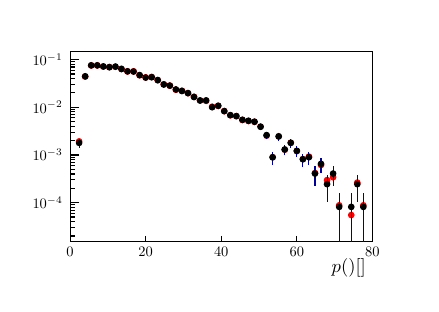
\begin{tikzpicture}
\pgfdeclareplotmark{cross} {
\pgfpathmoveto{\pgfpoint{-0.3\pgfplotmarksize}{\pgfplotmarksize}}
\pgfpathlineto{\pgfpoint{+0.3\pgfplotmarksize}{\pgfplotmarksize}}
\pgfpathlineto{\pgfpoint{+0.3\pgfplotmarksize}{0.3\pgfplotmarksize}}
\pgfpathlineto{\pgfpoint{+1\pgfplotmarksize}{0.3\pgfplotmarksize}}
\pgfpathlineto{\pgfpoint{+1\pgfplotmarksize}{-0.3\pgfplotmarksize}}
\pgfpathlineto{\pgfpoint{+0.3\pgfplotmarksize}{-0.3\pgfplotmarksize}}
\pgfpathlineto{\pgfpoint{+0.3\pgfplotmarksize}{-1.\pgfplotmarksize}}
\pgfpathlineto{\pgfpoint{-0.3\pgfplotmarksize}{-1.\pgfplotmarksize}}
\pgfpathlineto{\pgfpoint{-0.3\pgfplotmarksize}{-0.3\pgfplotmarksize}}
\pgfpathlineto{\pgfpoint{-1.\pgfplotmarksize}{-0.3\pgfplotmarksize}}
\pgfpathlineto{\pgfpoint{-1.\pgfplotmarksize}{0.3\pgfplotmarksize}}
\pgfpathlineto{\pgfpoint{-0.3\pgfplotmarksize}{0.3\pgfplotmarksize}}
\pgfpathclose
\pgfusepathqstroke
}
\pgfdeclareplotmark{cross*} {
\pgfpathmoveto{\pgfpoint{-0.3\pgfplotmarksize}{\pgfplotmarksize}}
\pgfpathlineto{\pgfpoint{+0.3\pgfplotmarksize}{\pgfplotmarksize}}
\pgfpathlineto{\pgfpoint{+0.3\pgfplotmarksize}{0.3\pgfplotmarksize}}
\pgfpathlineto{\pgfpoint{+1\pgfplotmarksize}{0.3\pgfplotmarksize}}
\pgfpathlineto{\pgfpoint{+1\pgfplotmarksize}{-0.3\pgfplotmarksize}}
\pgfpathlineto{\pgfpoint{+0.3\pgfplotmarksize}{-0.3\pgfplotmarksize}}
\pgfpathlineto{\pgfpoint{+0.3\pgfplotmarksize}{-1.\pgfplotmarksize}}
\pgfpathlineto{\pgfpoint{-0.3\pgfplotmarksize}{-1.\pgfplotmarksize}}
\pgfpathlineto{\pgfpoint{-0.3\pgfplotmarksize}{-0.3\pgfplotmarksize}}
\pgfpathlineto{\pgfpoint{-1.\pgfplotmarksize}{-0.3\pgfplotmarksize}}
\pgfpathlineto{\pgfpoint{-1.\pgfplotmarksize}{0.3\pgfplotmarksize}}
\pgfpathlineto{\pgfpoint{-0.3\pgfplotmarksize}{0.3\pgfplotmarksize}}
\pgfpathclose
\pgfusepathqfillstroke
}
\pgfdeclareplotmark{newstar} {
\pgfpathmoveto{\pgfqpoint{0pt}{\pgfplotmarksize}}
\pgfpathlineto{\pgfqpointpolar{44}{0.5\pgfplotmarksize}}
\pgfpathlineto{\pgfqpointpolar{18}{\pgfplotmarksize}}
\pgfpathlineto{\pgfqpointpolar{-20}{0.5\pgfplotmarksize}}
\pgfpathlineto{\pgfqpointpolar{-54}{\pgfplotmarksize}}
\pgfpathlineto{\pgfqpointpolar{-90}{0.5\pgfplotmarksize}}
\pgfpathlineto{\pgfqpointpolar{234}{\pgfplotmarksize}}
\pgfpathlineto{\pgfqpointpolar{198}{0.5\pgfplotmarksize}}
\pgfpathlineto{\pgfqpointpolar{162}{\pgfplotmarksize}}
\pgfpathlineto{\pgfqpointpolar{134}{0.5\pgfplotmarksize}}
\pgfpathclose
\pgfusepathqstroke
}
\pgfdeclareplotmark{newstar*} {
\pgfpathmoveto{\pgfqpoint{0pt}{\pgfplotmarksize}}
\pgfpathlineto{\pgfqpointpolar{44}{0.5\pgfplotmarksize}}
\pgfpathlineto{\pgfqpointpolar{18}{\pgfplotmarksize}}
\pgfpathlineto{\pgfqpointpolar{-20}{0.5\pgfplotmarksize}}
\pgfpathlineto{\pgfqpointpolar{-54}{\pgfplotmarksize}}
\pgfpathlineto{\pgfqpointpolar{-90}{0.5\pgfplotmarksize}}
\pgfpathlineto{\pgfqpointpolar{234}{\pgfplotmarksize}}
\pgfpathlineto{\pgfqpointpolar{198}{0.5\pgfplotmarksize}}
\pgfpathlineto{\pgfqpointpolar{162}{\pgfplotmarksize}}
\pgfpathlineto{\pgfqpointpolar{134}{0.5\pgfplotmarksize}}
\pgfpathclose
\pgfusepathqfillstroke
}
\definecolor{c}{rgb}{1,1,1};
\draw [color=c, fill=c] (0.1,0.0627517) rectangle (4.9,3.07483);
\draw [color=c, fill=c] (0.58,0.36396) rectangle (4.42,2.77362);
\definecolor{c}{rgb}{0,0,0};
\draw [c] (0.58,0.36396) -- (0.58,2.77362) -- (4.42,2.77362) -- (4.42,0.36396) -- (0.58,0.36396);
\definecolor{c}{rgb}{1,0,0};
\draw [c] (0.6952,1.61688) -- (0.6952,1.63756);
\draw [c] (0.6952,1.63756) -- (0.6952,1.65673);
\draw [c] (0.6568,1.63756) -- (0.6952,1.63756);
\draw [c] (0.6952,1.63756) -- (0.7336,1.63756);
\foreach \P in {(0.6952,1.63756)}{\draw[mark options={color=c,fill=c},mark size=2.402402pt,mark=*,mark size=1pt] plot coordinates {\P};}
\draw [c] (0.772,2.45646) -- (0.772,2.46065);
\draw [c] (0.772,2.46065) -- (0.772,2.46478);
\draw [c] (0.7336,2.46065) -- (0.772,2.46065);
\draw [c] (0.772,2.46065) -- (0.8104,2.46065);
\foreach \P in {(0.772,2.46065)}{\draw[mark options={color=c,fill=c},mark size=2.402402pt,mark=*,mark size=1pt] plot coordinates {\P};}
\draw [c] (0.8488,2.59887) -- (0.8488,2.60207);
\draw [c] (0.8488,2.60207) -- (0.8488,2.60523);
\draw [c] (0.8104,2.60207) -- (0.8488,2.60207);
\draw [c] (0.8488,2.60207) -- (0.8872,2.60207);
\foreach \P in {(0.8488,2.60207)}{\draw[mark options={color=c,fill=c},mark size=2.402402pt,mark=*,mark size=1pt] plot coordinates {\P};}
\draw [c] (0.9256,2.59914) -- (0.9256,2.60234);
\draw [c] (0.9256,2.60234) -- (0.9256,2.6055);
\draw [c] (0.8872,2.60234) -- (0.9256,2.60234);
\draw [c] (0.9256,2.60234) -- (0.964,2.60234);
\foreach \P in {(0.9256,2.60234)}{\draw[mark options={color=c,fill=c},mark size=2.402402pt,mark=*,mark size=1pt] plot coordinates {\P};}
\draw [c] (1.0024,2.58506) -- (1.0024,2.58834);
\draw [c] (1.0024,2.58834) -- (1.0024,2.59159);
\draw [c] (0.964,2.58834) -- (1.0024,2.58834);
\draw [c] (1.0024,2.58834) -- (1.0408,2.58834);
\foreach \P in {(1.0024,2.58834)}{\draw[mark options={color=c,fill=c},mark size=2.402402pt,mark=*,mark size=1pt] plot coordinates {\P};}
\draw [c] (1.0792,2.57929) -- (1.0792,2.58261);
\draw [c] (1.0792,2.58261) -- (1.0792,2.58589);
\draw [c] (1.0408,2.58261) -- (1.0792,2.58261);
\draw [c] (1.0792,2.58261) -- (1.1176,2.58261);
\foreach \P in {(1.0792,2.58261)}{\draw[mark options={color=c,fill=c},mark size=2.402402pt,mark=*,mark size=1pt] plot coordinates {\P};}
\draw [c] (1.156,2.58231) -- (1.156,2.58562);
\draw [c] (1.156,2.58562) -- (1.156,2.58888);
\draw [c] (1.1176,2.58562) -- (1.156,2.58562);
\draw [c] (1.156,2.58562) -- (1.1944,2.58562);
\foreach \P in {(1.156,2.58562)}{\draw[mark options={color=c,fill=c},mark size=2.402402pt,mark=*,mark size=1pt] plot coordinates {\P};}
\draw [c] (1.2328,2.55619) -- (1.2328,2.55966);
\draw [c] (1.2328,2.55966) -- (1.2328,2.56309);
\draw [c] (1.1944,2.55966) -- (1.2328,2.55966);
\draw [c] (1.2328,2.55966) -- (1.2712,2.55966);
\foreach \P in {(1.2328,2.55966)}{\draw[mark options={color=c,fill=c},mark size=2.402402pt,mark=*,mark size=1pt] plot coordinates {\P};}
\draw [c] (1.3096,2.52233) -- (1.3096,2.52603);
\draw [c] (1.3096,2.52603) -- (1.3096,2.52968);
\draw [c] (1.2712,2.52603) -- (1.3096,2.52603);
\draw [c] (1.3096,2.52603) -- (1.348,2.52603);
\foreach \P in {(1.3096,2.52603)}{\draw[mark options={color=c,fill=c},mark size=2.402402pt,mark=*,mark size=1pt] plot coordinates {\P};}
\draw [c] (1.3864,2.52326) -- (1.3864,2.52695);
\draw [c] (1.3864,2.52695) -- (1.3864,2.5306);
\draw [c] (1.348,2.52695) -- (1.3864,2.52695);
\draw [c] (1.3864,2.52695) -- (1.4248,2.52695);
\foreach \P in {(1.3864,2.52695)}{\draw[mark options={color=c,fill=c},mark size=2.402402pt,mark=*,mark size=1pt] plot coordinates {\P};}
\draw [c] (1.4632,2.4726) -- (1.4632,2.47667);
\draw [c] (1.4632,2.47667) -- (1.4632,2.48067);
\draw [c] (1.4248,2.47667) -- (1.4632,2.47667);
\draw [c] (1.4632,2.47667) -- (1.5016,2.47667);
\foreach \P in {(1.4632,2.47667)}{\draw[mark options={color=c,fill=c},mark size=2.402402pt,mark=*,mark size=1pt] plot coordinates {\P};}
\draw [c] (1.54,2.44652) -- (1.54,2.4508);
\draw [c] (1.54,2.4508) -- (1.54,2.455);
\draw [c] (1.5016,2.4508) -- (1.54,2.4508);
\draw [c] (1.54,2.4508) -- (1.5784,2.4508);
\foreach \P in {(1.54,2.4508)}{\draw[mark options={color=c,fill=c},mark size=2.402402pt,mark=*,mark size=1pt] plot coordinates {\P};}
\draw [c] (1.6168,2.45171) -- (1.6168,2.45594);
\draw [c] (1.6168,2.45594) -- (1.6168,2.4601);
\draw [c] (1.5784,2.45594) -- (1.6168,2.45594);
\draw [c] (1.6168,2.45594) -- (1.6552,2.45594);
\foreach \P in {(1.6168,2.45594)}{\draw[mark options={color=c,fill=c},mark size=2.402402pt,mark=*,mark size=1pt] plot coordinates {\P};}
\draw [c] (1.6936,2.40843) -- (1.6936,2.41303);
\draw [c] (1.6936,2.41303) -- (1.6936,2.41754);
\draw [c] (1.6552,2.41303) -- (1.6936,2.41303);
\draw [c] (1.6936,2.41303) -- (1.732,2.41303);
\foreach \P in {(1.6936,2.41303)}{\draw[mark options={color=c,fill=c},mark size=2.402402pt,mark=*,mark size=1pt] plot coordinates {\P};}
\draw [c] (1.7704,2.35821) -- (1.7704,2.36326);
\draw [c] (1.7704,2.36326) -- (1.7704,2.36822);
\draw [c] (1.732,2.36326) -- (1.7704,2.36326);
\draw [c] (1.7704,2.36326) -- (1.8088,2.36326);
\foreach \P in {(1.7704,2.36326)}{\draw[mark options={color=c,fill=c},mark size=2.402402pt,mark=*,mark size=1pt] plot coordinates {\P};}
\draw [c] (1.8472,2.33978) -- (1.8472,2.34502);
\draw [c] (1.8472,2.34502) -- (1.8472,2.35015);
\draw [c] (1.8088,2.34502) -- (1.8472,2.34502);
\draw [c] (1.8472,2.34502) -- (1.8856,2.34502);
\foreach \P in {(1.8472,2.34502)}{\draw[mark options={color=c,fill=c},mark size=2.402402pt,mark=*,mark size=1pt] plot coordinates {\P};}
\draw [c] (1.924,2.28774) -- (1.924,2.29352);
\draw [c] (1.924,2.29352) -- (1.924,2.29917);
\draw [c] (1.8856,2.29352) -- (1.924,2.29352);
\draw [c] (1.924,2.29352) -- (1.9624,2.29352);
\foreach \P in {(1.924,2.29352)}{\draw[mark options={color=c,fill=c},mark size=2.402402pt,mark=*,mark size=1pt] plot coordinates {\P};}
\draw [c] (2.0008,2.275) -- (2.0008,2.28092);
\draw [c] (2.0008,2.28092) -- (2.0008,2.28671);
\draw [c] (1.9624,2.28092) -- (2.0008,2.28092);
\draw [c] (2.0008,2.28092) -- (2.0392,2.28092);
\foreach \P in {(2.0008,2.28092)}{\draw[mark options={color=c,fill=c},mark size=2.402402pt,mark=*,mark size=1pt] plot coordinates {\P};}
\draw [c] (2.0776,2.24341) -- (2.0776,2.24969);
\draw [c] (2.0776,2.24969) -- (2.0776,2.25583);
\draw [c] (2.0392,2.24969) -- (2.0776,2.24969);
\draw [c] (2.0776,2.24969) -- (2.116,2.24969);
\foreach \P in {(2.0776,2.24969)}{\draw[mark options={color=c,fill=c},mark size=2.402402pt,mark=*,mark size=1pt] plot coordinates {\P};}
\draw [c] (2.1544,2.19747) -- (2.1544,2.20433);
\draw [c] (2.1544,2.20433) -- (2.1544,2.21101);
\draw [c] (2.116,2.20433) -- (2.1544,2.20433);
\draw [c] (2.1544,2.20433) -- (2.1928,2.20433);
\foreach \P in {(2.1544,2.20433)}{\draw[mark options={color=c,fill=c},mark size=2.402402pt,mark=*,mark size=1pt] plot coordinates {\P};}
\draw [c] (2.2312,2.15) -- (2.2312,2.15751);
\draw [c] (2.2312,2.15751) -- (2.2312,2.16481);
\draw [c] (2.1928,2.15751) -- (2.2312,2.15751);
\draw [c] (2.2312,2.15751) -- (2.2696,2.15751);
\foreach \P in {(2.2312,2.15751)}{\draw[mark options={color=c,fill=c},mark size=2.402402pt,mark=*,mark size=1pt] plot coordinates {\P};}
\draw [c] (2.308,2.14467) -- (2.308,2.15225);
\draw [c] (2.308,2.15225) -- (2.308,2.15963);
\draw [c] (2.2696,2.15225) -- (2.308,2.15225);
\draw [c] (2.308,2.15225) -- (2.3464,2.15225);
\foreach \P in {(2.308,2.15225)}{\draw[mark options={color=c,fill=c},mark size=2.402402pt,mark=*,mark size=1pt] plot coordinates {\P};}
\draw [c] (2.3848,2.06909) -- (2.3848,2.07784);
\draw [c] (2.3848,2.07784) -- (2.3848,2.08632);
\draw [c] (2.3464,2.07784) -- (2.3848,2.07784);
\draw [c] (2.3848,2.07784) -- (2.4232,2.07784);
\foreach \P in {(2.3848,2.07784)}{\draw[mark options={color=c,fill=c},mark size=2.402402pt,mark=*,mark size=1pt] plot coordinates {\P};}
\draw [c] (2.4616,2.07949) -- (2.4616,2.08807);
\draw [c] (2.4616,2.08807) -- (2.4616,2.09639);
\draw [c] (2.4232,2.08807) -- (2.4616,2.08807);
\draw [c] (2.4616,2.08807) -- (2.5,2.08807);
\foreach \P in {(2.4616,2.08807)}{\draw[mark options={color=c,fill=c},mark size=2.402402pt,mark=*,mark size=1pt] plot coordinates {\P};}
\draw [c] (2.5384,2.01169) -- (2.5384,2.02146);
\draw [c] (2.5384,2.02146) -- (2.5384,2.03087);
\draw [c] (2.5,2.02146) -- (2.5384,2.02146);
\draw [c] (2.5384,2.02146) -- (2.5768,2.02146);
\foreach \P in {(2.5384,2.02146)}{\draw[mark options={color=c,fill=c},mark size=2.402402pt,mark=*,mark size=1pt] plot coordinates {\P};}
\draw [c] (2.6152,1.95737) -- (2.6152,1.9682);
\draw [c] (2.6152,1.9682) -- (2.6152,1.9786);
\draw [c] (2.5768,1.9682) -- (2.6152,1.9682);
\draw [c] (2.6152,1.9682) -- (2.6536,1.9682);
\foreach \P in {(2.6152,1.9682)}{\draw[mark options={color=c,fill=c},mark size=2.402402pt,mark=*,mark size=1pt] plot coordinates {\P};}
\draw [c] (2.692,1.94759) -- (2.692,1.95862);
\draw [c] (2.692,1.95862) -- (2.692,1.9692);
\draw [c] (2.6536,1.95862) -- (2.692,1.95862);
\draw [c] (2.692,1.95862) -- (2.7304,1.95862);
\foreach \P in {(2.692,1.95862)}{\draw[mark options={color=c,fill=c},mark size=2.402402pt,mark=*,mark size=1pt] plot coordinates {\P};}
\draw [c] (2.7688,1.89736) -- (2.7688,1.9095);
\draw [c] (2.7688,1.9095) -- (2.7688,1.9211);
\draw [c] (2.7304,1.9095) -- (2.7688,1.9095);
\draw [c] (2.7688,1.9095) -- (2.8072,1.9095);
\foreach \P in {(2.7688,1.9095)}{\draw[mark options={color=c,fill=c},mark size=2.402402pt,mark=*,mark size=1pt] plot coordinates {\P};}
\draw [c] (2.8456,1.88389) -- (2.8456,1.89634);
\draw [c] (2.8456,1.89634) -- (2.8456,1.90823);
\draw [c] (2.8072,1.89634) -- (2.8456,1.89634);
\draw [c] (2.8456,1.89634) -- (2.884,1.89634);
\foreach \P in {(2.8456,1.89634)}{\draw[mark options={color=c,fill=c},mark size=2.402402pt,mark=*,mark size=1pt] plot coordinates {\P};}
\draw [c] (2.9224,1.87392) -- (2.9224,1.88661);
\draw [c] (2.9224,1.88661) -- (2.9224,1.89871);
\draw [c] (2.884,1.88661) -- (2.9224,1.88661);
\draw [c] (2.9224,1.88661) -- (2.9608,1.88661);
\foreach \P in {(2.9224,1.88661)}{\draw[mark options={color=c,fill=c},mark size=2.402402pt,mark=*,mark size=1pt] plot coordinates {\P};}
\draw [c] (2.9992,1.81006) -- (2.9992,1.82438);
\draw [c] (2.9992,1.82438) -- (2.9992,1.83797);
\draw [c] (2.9608,1.82438) -- (2.9992,1.82438);
\draw [c] (2.9992,1.82438) -- (3.0376,1.82438);
\foreach \P in {(2.9992,1.82438)}{\draw[mark options={color=c,fill=c},mark size=2.402402pt,mark=*,mark size=1pt] plot coordinates {\P};}
\draw [c] (3.076,1.69151) -- (3.076,1.70946);
\draw [c] (3.076,1.70946) -- (3.076,1.72626);
\draw [c] (3.0376,1.70946) -- (3.076,1.70946);
\draw [c] (3.076,1.70946) -- (3.1144,1.70946);
\foreach \P in {(3.076,1.70946)}{\draw[mark options={color=c,fill=c},mark size=2.402402pt,mark=*,mark size=1pt] plot coordinates {\P};}
\draw [c] (3.1528,1.40392) -- (3.1528,1.43491);
\draw [c] (3.1528,1.43491) -- (3.1528,1.46263);
\draw [c] (3.1144,1.43491) -- (3.1528,1.43491);
\draw [c] (3.1528,1.43491) -- (3.1912,1.43491);
\foreach \P in {(3.1528,1.43491)}{\draw[mark options={color=c,fill=c},mark size=2.402402pt,mark=*,mark size=1pt] plot coordinates {\P};}
\draw [c] (3.2296,1.68431) -- (3.2296,1.7025);
\draw [c] (3.2296,1.7025) -- (3.2296,1.71952);
\draw [c] (3.1912,1.7025) -- (3.2296,1.7025);
\draw [c] (3.2296,1.7025) -- (3.268,1.7025);
\foreach \P in {(3.2296,1.7025)}{\draw[mark options={color=c,fill=c},mark size=2.402402pt,mark=*,mark size=1pt] plot coordinates {\P};}
\draw [c] (3.3064,1.50613) -- (3.3064,1.53165);
\draw [c] (3.3064,1.53165) -- (3.3064,1.55491);
\draw [c] (3.268,1.53165) -- (3.3064,1.53165);
\draw [c] (3.3064,1.53165) -- (3.3448,1.53165);
\foreach \P in {(3.3064,1.53165)}{\draw[mark options={color=c,fill=c},mark size=2.402402pt,mark=*,mark size=1pt] plot coordinates {\P};}
\draw [c] (3.3832,1.59909) -- (3.3832,1.62048);
\draw [c] (3.3832,1.62048) -- (3.3832,1.64026);
\draw [c] (3.3448,1.62048) -- (3.3832,1.62048);
\draw [c] (3.3832,1.62048) -- (3.4216,1.62048);
\foreach \P in {(3.3832,1.62048)}{\draw[mark options={color=c,fill=c},mark size=2.402402pt,mark=*,mark size=1pt] plot coordinates {\P};}
\draw [c] (3.46,1.48653) -- (3.46,1.51301);
\draw [c] (3.46,1.51301) -- (3.46,1.53708);
\draw [c] (3.4216,1.51301) -- (3.46,1.51301);
\draw [c] (3.46,1.51301) -- (3.4984,1.51301);
\foreach \P in {(3.46,1.51301)}{\draw[mark options={color=c,fill=c},mark size=2.402402pt,mark=*,mark size=1pt] plot coordinates {\P};}
\draw [c] (3.5368,1.37862) -- (3.5368,1.41113);
\draw [c] (3.5368,1.41113) -- (3.5368,1.44006);
\draw [c] (3.4984,1.41113) -- (3.5368,1.41113);
\draw [c] (3.5368,1.41113) -- (3.5752,1.41113);
\foreach \P in {(3.5368,1.41113)}{\draw[mark options={color=c,fill=c},mark size=2.402402pt,mark=*,mark size=1pt] plot coordinates {\P};}
\draw [c] (3.6136,1.41408) -- (3.6136,1.44448);
\draw [c] (3.6136,1.44448) -- (3.6136,1.47172);
\draw [c] (3.5752,1.44448) -- (3.6136,1.44448);
\draw [c] (3.6136,1.44448) -- (3.652,1.44448);
\foreach \P in {(3.6136,1.44448)}{\draw[mark options={color=c,fill=c},mark size=2.402402pt,mark=*,mark size=1pt] plot coordinates {\P};}
\draw [c] (3.6904,1.18924) -- (3.6904,1.2358);
\draw [c] (3.6904,1.2358) -- (3.6904,1.27535);
\draw [c] (3.652,1.2358) -- (3.6904,1.2358);
\draw [c] (3.6904,1.2358) -- (3.7288,1.2358);
\foreach \P in {(3.6904,1.2358)}{\draw[mark options={color=c,fill=c},mark size=2.402402pt,mark=*,mark size=1pt] plot coordinates {\P};}
\draw [c] (3.7672,1.30007) -- (3.7672,1.33781);
\draw [c] (3.7672,1.33781) -- (3.7672,1.37081);
\draw [c] (3.7288,1.33781) -- (3.7672,1.33781);
\draw [c] (3.7672,1.33781) -- (3.8056,1.33781);
\foreach \P in {(3.7672,1.33781)}{\draw[mark options={color=c,fill=c},mark size=2.402402pt,mark=*,mark size=1pt] plot coordinates {\P};}
\draw [c] (3.844,1.08966) -- (3.844,1.1459);
\draw [c] (3.844,1.1459) -- (3.844,1.1922);
\draw [c] (3.8056,1.1459) -- (3.844,1.1459);
\draw [c] (3.844,1.1459) -- (3.8824,1.1459);
\foreach \P in {(3.844,1.1459)}{\draw[mark options={color=c,fill=c},mark size=2.402402pt,mark=*,mark size=1pt] plot coordinates {\P};}
\draw [c] (3.9208,1.13016) -- (3.9208,1.18224);
\draw [c] (3.9208,1.18224) -- (3.9208,1.22569);
\draw [c] (3.8824,1.18224) -- (3.9208,1.18224);
\draw [c] (3.9208,1.18224) -- (3.9592,1.18224);
\foreach \P in {(3.9208,1.18224)}{\draw[mark options={color=c,fill=c},mark size=2.402402pt,mark=*,mark size=1pt] plot coordinates {\P};}
\draw [c] (3.9976,0.711127) -- (3.9976,0.825896);
\draw [c] (3.9976,0.825896) -- (3.9976,0.905537);
\draw [c] (3.9592,0.825896) -- (3.9976,0.825896);
\draw [c] (3.9976,0.825896) -- (4.036,0.825896);
\foreach \P in {(3.9976,0.825896)}{\draw[mark options={color=c,fill=c},mark size=2.402402pt,mark=*,mark size=1pt] plot coordinates {\P};}
\draw [c] (4.1512,0.546307) -- (4.1512,0.702251);
\draw [c] (4.1512,0.702251) -- (4.1512,0.799493);
\draw [c] (4.1128,0.702251) -- (4.1512,0.702251);
\draw [c] (4.1512,0.702251) -- (4.1896,0.702251);
\foreach \P in {(4.1512,0.702251)}{\draw[mark options={color=c,fill=c},mark size=2.402402pt,mark=*,mark size=1pt] plot coordinates {\P};}
\draw [c] (4.228,1.05485) -- (4.228,1.11491);
\draw [c] (4.228,1.11491) -- (4.228,1.16378);
\draw [c] (4.1896,1.11491) -- (4.228,1.11491);
\draw [c] (4.228,1.11491) -- (4.2664,1.11491);
\foreach \P in {(4.228,1.11491)}{\draw[mark options={color=c,fill=c},mark size=2.402402pt,mark=*,mark size=1pt] plot coordinates {\P};}
\draw [c] (4.3048,0.711127) -- (4.3048,0.825896);
\draw [c] (4.3048,0.825896) -- (4.3048,0.905537);
\draw [c] (4.2664,0.825896) -- (4.3048,0.825896);
\draw [c] (4.3048,0.825896) -- (4.3432,0.825896);
\foreach \P in {(4.3048,0.825896)}{\draw[mark options={color=c,fill=c},mark size=2.402402pt,mark=*,mark size=1pt] plot coordinates {\P};}
\definecolor{c}{rgb}{0,0,0};
\draw [c] (0.58,0.36396) -- (4.42,0.36396);
\draw [anchor= east] (4.42,0.0266067) node[scale=0.672711, rotate=0]{$p(\kaon) [\mevc]$};
\draw [c] (0.58,0.43625) -- (0.58,0.36396);
\draw [c] (1.54,0.43625) -- (1.54,0.36396);
\draw [c] (2.5,0.43625) -- (2.5,0.36396);
\draw [c] (3.46,0.43625) -- (3.46,0.36396);
\draw [c] (4.42,0.43625) -- (4.42,0.36396);
\draw [anchor=base] (0.58,0.171187) node[scale=0.52322, rotate=0]{0};
\draw [anchor=base] (1.54,0.171187) node[scale=0.52322, rotate=0]{20};
\draw [anchor=base] (2.5,0.171187) node[scale=0.52322, rotate=0]{40};
\draw [anchor=base] (3.46,0.171187) node[scale=0.52322, rotate=0]{60};
\draw [anchor=base] (4.42,0.171187) node[scale=0.52322, rotate=0]{80};
\draw [c] (0.58,0.36396) -- (0.58,2.77362);
\draw [c] (0.6376,0.435798) -- (0.58,0.435798);
\draw [c] (0.6376,0.542465) -- (0.58,0.542465);
\draw [c] (0.6376,0.618146) -- (0.58,0.618146);
\draw [c] (0.6376,0.676848) -- (0.58,0.676848);
\draw [c] (0.6376,0.724812) -- (0.58,0.724812);
\draw [c] (0.6376,0.765365) -- (0.58,0.765365);
\draw [c] (0.6376,0.800493) -- (0.58,0.800493);
\draw [c] (0.6376,0.831478) -- (0.58,0.831478);
\draw [c] (0.6952,0.859196) -- (0.58,0.859196);
\draw [anchor= east] (0.54928,0.859196) node[scale=0.52322, rotate=0]{$10^{-4}$};
\draw [c] (0.6376,1.04154) -- (0.58,1.04154);
\draw [c] (0.6376,1.14821) -- (0.58,1.14821);
\draw [c] (0.6376,1.22389) -- (0.58,1.22389);
\draw [c] (0.6376,1.28259) -- (0.58,1.28259);
\draw [c] (0.6376,1.33056) -- (0.58,1.33056);
\draw [c] (0.6376,1.37111) -- (0.58,1.37111);
\draw [c] (0.6376,1.40624) -- (0.58,1.40624);
\draw [c] (0.6376,1.43722) -- (0.58,1.43722);
\draw [c] (0.6952,1.46494) -- (0.58,1.46494);
\draw [anchor= east] (0.54928,1.46494) node[scale=0.52322, rotate=0]{$10^{-3}$};
\draw [c] (0.6376,1.64729) -- (0.58,1.64729);
\draw [c] (0.6376,1.75395) -- (0.58,1.75395);
\draw [c] (0.6376,1.82963) -- (0.58,1.82963);
\draw [c] (0.6376,1.88834) -- (0.58,1.88834);
\draw [c] (0.6376,1.9363) -- (0.58,1.9363);
\draw [c] (0.6376,1.97685) -- (0.58,1.97685);
\draw [c] (0.6376,2.01198) -- (0.58,2.01198);
\draw [c] (0.6376,2.04297) -- (0.58,2.04297);
\draw [c] (0.6952,2.07068) -- (0.58,2.07068);
\draw [anchor= east] (0.54928,2.07068) node[scale=0.52322, rotate=0]{$10^{-2}$};
\draw [c] (0.6376,2.25303) -- (0.58,2.25303);
\draw [c] (0.6376,2.3597) -- (0.58,2.3597);
\draw [c] (0.6376,2.43538) -- (0.58,2.43538);
\draw [c] (0.6376,2.49408) -- (0.58,2.49408);
\draw [c] (0.6376,2.54204) -- (0.58,2.54204);
\draw [c] (0.6376,2.5826) -- (0.58,2.5826);
\draw [c] (0.6376,2.61773) -- (0.58,2.61773);
\draw [c] (0.6376,2.64871) -- (0.58,2.64871);
\draw [c] (0.6952,2.67643) -- (0.58,2.67643);
\draw [anchor= east] (0.54928,2.67643) node[scale=0.52322, rotate=0]{$10^{-1}$};
\definecolor{c}{rgb}{0,0,0.6};
\draw [c] (0.6952,1.55576) -- (0.6952,1.61884);
\draw [c] (0.6952,1.61884) -- (0.6952,1.66969);
\draw [c] (0.6568,1.61884) -- (0.6952,1.61884);
\draw [c] (0.6952,1.61884) -- (0.7336,1.61884);
\definecolor{c}{rgb}{0,0,0};
\foreach \P in {(0.6952,1.61884)}{\draw[mark options={color=c,fill=c},mark size=2.402402pt,mark=*,mark size=1pt] plot coordinates {\P};}
\definecolor{c}{rgb}{0,0,0.6};
\draw [c] (0.772,2.4527) -- (0.772,2.4642);
\draw [c] (0.772,2.4642) -- (0.772,2.47521);
\draw [c] (0.7336,2.4642) -- (0.772,2.4642);
\draw [c] (0.772,2.4642) -- (0.8104,2.4642);
\definecolor{c}{rgb}{0,0,0};
\foreach \P in {(0.772,2.4642)}{\draw[mark options={color=c,fill=c},mark size=2.402402pt,mark=*,mark size=1pt] plot coordinates {\P};}
\definecolor{c}{rgb}{0,0,0.6};
\draw [c] (0.8488,2.59447) -- (0.8488,2.60325);
\draw [c] (0.8488,2.60325) -- (0.8488,2.61175);
\draw [c] (0.8104,2.60325) -- (0.8488,2.60325);
\draw [c] (0.8488,2.60325) -- (0.8872,2.60325);
\definecolor{c}{rgb}{0,0,0};
\foreach \P in {(0.8488,2.60325)}{\draw[mark options={color=c,fill=c},mark size=2.402402pt,mark=*,mark size=1pt] plot coordinates {\P};}
\definecolor{c}{rgb}{0,0,0.6};
\draw [c] (0.9256,2.59447) -- (0.9256,2.60325);
\draw [c] (0.9256,2.60325) -- (0.9256,2.61175);
\draw [c] (0.8872,2.60325) -- (0.9256,2.60325);
\draw [c] (0.9256,2.60325) -- (0.964,2.60325);
\definecolor{c}{rgb}{0,0,0};
\foreach \P in {(0.9256,2.60325)}{\draw[mark options={color=c,fill=c},mark size=2.402402pt,mark=*,mark size=1pt] plot coordinates {\P};}
\definecolor{c}{rgb}{0,0,0.6};
\draw [c] (1.0024,2.58057) -- (1.0024,2.58958);
\draw [c] (1.0024,2.58958) -- (1.0024,2.5983);
\draw [c] (0.964,2.58958) -- (1.0024,2.58958);
\draw [c] (1.0024,2.58958) -- (1.0408,2.58958);
\definecolor{c}{rgb}{0,0,0};
\foreach \P in {(1.0024,2.58958)}{\draw[mark options={color=c,fill=c},mark size=2.402402pt,mark=*,mark size=1pt] plot coordinates {\P};}
\definecolor{c}{rgb}{0,0,0.6};
\draw [c] (1.0792,2.57003) -- (1.0792,2.57923);
\draw [c] (1.0792,2.57923) -- (1.0792,2.58811);
\draw [c] (1.0408,2.57923) -- (1.0792,2.57923);
\draw [c] (1.0792,2.57923) -- (1.1176,2.57923);
\definecolor{c}{rgb}{0,0,0};
\foreach \P in {(1.0792,2.57923)}{\draw[mark options={color=c,fill=c},mark size=2.402402pt,mark=*,mark size=1pt] plot coordinates {\P};}
\definecolor{c}{rgb}{0,0,0.6};
\draw [c] (1.156,2.57843) -- (1.156,2.58748);
\draw [c] (1.156,2.58748) -- (1.156,2.59623);
\draw [c] (1.1176,2.58748) -- (1.156,2.58748);
\draw [c] (1.156,2.58748) -- (1.1944,2.58748);
\definecolor{c}{rgb}{0,0,0};
\foreach \P in {(1.156,2.58748)}{\draw[mark options={color=c,fill=c},mark size=2.402402pt,mark=*,mark size=1pt] plot coordinates {\P};}
\definecolor{c}{rgb}{0,0,0.6};
\draw [c] (1.2328,2.54658) -- (1.2328,2.5562);
\draw [c] (1.2328,2.5562) -- (1.2328,2.56547);
\draw [c] (1.1944,2.5562) -- (1.2328,2.5562);
\draw [c] (1.2328,2.5562) -- (1.2712,2.5562);
\definecolor{c}{rgb}{0,0,0};
\foreach \P in {(1.2328,2.5562)}{\draw[mark options={color=c,fill=c},mark size=2.402402pt,mark=*,mark size=1pt] plot coordinates {\P};}
\definecolor{c}{rgb}{0,0,0.6};
\draw [c] (1.3096,2.51702) -- (1.3096,2.52719);
\draw [c] (1.3096,2.52719) -- (1.3096,2.53699);
\draw [c] (1.2712,2.52719) -- (1.3096,2.52719);
\draw [c] (1.3096,2.52719) -- (1.348,2.52719);
\definecolor{c}{rgb}{0,0,0};
\foreach \P in {(1.3096,2.52719)}{\draw[mark options={color=c,fill=c},mark size=2.402402pt,mark=*,mark size=1pt] plot coordinates {\P};}
\definecolor{c}{rgb}{0,0,0.6};
\draw [c] (1.3864,2.51431) -- (1.3864,2.52453);
\draw [c] (1.3864,2.52453) -- (1.3864,2.53437);
\draw [c] (1.348,2.52453) -- (1.3864,2.52453);
\draw [c] (1.3864,2.52453) -- (1.4248,2.52453);
\definecolor{c}{rgb}{0,0,0};
\foreach \P in {(1.3864,2.52453)}{\draw[mark options={color=c,fill=c},mark size=2.402402pt,mark=*,mark size=1pt] plot coordinates {\P};}
\definecolor{c}{rgb}{0,0,0.6};
\draw [c] (1.4632,2.46845) -- (1.4632,2.47961);
\draw [c] (1.4632,2.47961) -- (1.4632,2.49031);
\draw [c] (1.4248,2.47961) -- (1.4632,2.47961);
\draw [c] (1.4632,2.47961) -- (1.5016,2.47961);
\definecolor{c}{rgb}{0,0,0};
\foreach \P in {(1.4632,2.47961)}{\draw[mark options={color=c,fill=c},mark size=2.402402pt,mark=*,mark size=1pt] plot coordinates {\P};}
\definecolor{c}{rgb}{0,0,0.6};
\draw [c] (1.54,2.43596) -- (1.54,2.44783);
\draw [c] (1.54,2.44783) -- (1.54,2.45918);
\draw [c] (1.5016,2.44783) -- (1.54,2.44783);
\draw [c] (1.54,2.44783) -- (1.5784,2.44783);
\definecolor{c}{rgb}{0,0,0};
\foreach \P in {(1.54,2.44783)}{\draw[mark options={color=c,fill=c},mark size=2.402402pt,mark=*,mark size=1pt] plot coordinates {\P};}
\definecolor{c}{rgb}{0,0,0.6};
\draw [c] (1.6168,2.44063) -- (1.6168,2.4524);
\draw [c] (1.6168,2.4524) -- (1.6168,2.46365);
\draw [c] (1.5784,2.4524) -- (1.6168,2.4524);
\draw [c] (1.6168,2.4524) -- (1.6552,2.4524);
\definecolor{c}{rgb}{0,0,0};
\foreach \P in {(1.6168,2.4524)}{\draw[mark options={color=c,fill=c},mark size=2.402402pt,mark=*,mark size=1pt] plot coordinates {\P};}
\definecolor{c}{rgb}{0,0,0.6};
\draw [c] (1.6936,2.4043) -- (1.6936,2.41691);
\draw [c] (1.6936,2.41691) -- (1.6936,2.42893);
\draw [c] (1.6552,2.41691) -- (1.6936,2.41691);
\draw [c] (1.6936,2.41691) -- (1.732,2.41691);
\definecolor{c}{rgb}{0,0,0};
\foreach \P in {(1.6936,2.41691)}{\draw[mark options={color=c,fill=c},mark size=2.402402pt,mark=*,mark size=1pt] plot coordinates {\P};}
\definecolor{c}{rgb}{0,0,0.6};
\draw [c] (1.7704,2.34584) -- (1.7704,2.35993);
\draw [c] (1.7704,2.35993) -- (1.7704,2.37329);
\draw [c] (1.732,2.35993) -- (1.7704,2.35993);
\draw [c] (1.7704,2.35993) -- (1.8088,2.35993);
\definecolor{c}{rgb}{0,0,0};
\foreach \P in {(1.7704,2.35993)}{\draw[mark options={color=c,fill=c},mark size=2.402402pt,mark=*,mark size=1pt] plot coordinates {\P};}
\definecolor{c}{rgb}{0,0,0.6};
\draw [c] (1.8472,2.33151) -- (1.8472,2.34598);
\draw [c] (1.8472,2.34598) -- (1.8472,2.3597);
\draw [c] (1.8088,2.34598) -- (1.8472,2.34598);
\draw [c] (1.8472,2.34598) -- (1.8856,2.34598);
\definecolor{c}{rgb}{0,0,0};
\foreach \P in {(1.8472,2.34598)}{\draw[mark options={color=c,fill=c},mark size=2.402402pt,mark=*,mark size=1pt] plot coordinates {\P};}
\definecolor{c}{rgb}{0,0,0.6};
\draw [c] (1.924,2.28134) -- (1.924,2.29726);
\draw [c] (1.924,2.29726) -- (1.924,2.31227);
\draw [c] (1.8856,2.29726) -- (1.924,2.29726);
\draw [c] (1.924,2.29726) -- (1.9624,2.29726);
\definecolor{c}{rgb}{0,0,0};
\foreach \P in {(1.924,2.29726)}{\draw[mark options={color=c,fill=c},mark size=2.402402pt,mark=*,mark size=1pt] plot coordinates {\P};}
\definecolor{c}{rgb}{0,0,0.6};
\draw [c] (2.0008,2.26094) -- (2.0008,2.27749);
\draw [c] (2.0008,2.27749) -- (2.0008,2.29306);
\draw [c] (1.9624,2.27749) -- (2.0008,2.27749);
\draw [c] (2.0008,2.27749) -- (2.0392,2.27749);
\definecolor{c}{rgb}{0,0,0};
\foreach \P in {(2.0008,2.27749)}{\draw[mark options={color=c,fill=c},mark size=2.402402pt,mark=*,mark size=1pt] plot coordinates {\P};}
\definecolor{c}{rgb}{0,0,0.6};
\draw [c] (2.0776,2.2333) -- (2.0776,2.25075);
\draw [c] (2.0776,2.25075) -- (2.0776,2.2671);
\draw [c] (2.0392,2.25075) -- (2.0776,2.25075);
\draw [c] (2.0776,2.25075) -- (2.116,2.25075);
\definecolor{c}{rgb}{0,0,0};
\foreach \P in {(2.0776,2.25075)}{\draw[mark options={color=c,fill=c},mark size=2.402402pt,mark=*,mark size=1pt] plot coordinates {\P};}
\definecolor{c}{rgb}{0,0,0.6};
\draw [c] (2.1544,2.18158) -- (2.1544,2.20083);
\draw [c] (2.1544,2.20083) -- (2.1544,2.21876);
\draw [c] (2.116,2.20083) -- (2.1544,2.20083);
\draw [c] (2.1544,2.20083) -- (2.1928,2.20083);
\definecolor{c}{rgb}{0,0,0};
\foreach \P in {(2.1544,2.20083)}{\draw[mark options={color=c,fill=c},mark size=2.402402pt,mark=*,mark size=1pt] plot coordinates {\P};}
\definecolor{c}{rgb}{0,0,0.6};
\draw [c] (2.2312,2.13577) -- (2.2312,2.15676);
\draw [c] (2.2312,2.15676) -- (2.2312,2.1762);
\draw [c] (2.1928,2.15676) -- (2.2312,2.15676);
\draw [c] (2.2312,2.15676) -- (2.2696,2.15676);
\definecolor{c}{rgb}{0,0,0};
\foreach \P in {(2.2312,2.15676)}{\draw[mark options={color=c,fill=c},mark size=2.402402pt,mark=*,mark size=1pt] plot coordinates {\P};}
\definecolor{c}{rgb}{0,0,0.6};
\draw [c] (2.308,2.13738) -- (2.308,2.1583);
\draw [c] (2.308,2.1583) -- (2.308,2.17769);
\draw [c] (2.2696,2.1583) -- (2.308,2.1583);
\draw [c] (2.308,2.1583) -- (2.3464,2.1583);
\definecolor{c}{rgb}{0,0,0};
\foreach \P in {(2.308,2.1583)}{\draw[mark options={color=c,fill=c},mark size=2.402402pt,mark=*,mark size=1pt] plot coordinates {\P};}
\definecolor{c}{rgb}{0,0,0.6};
\draw [c] (2.3848,2.04677) -- (2.3848,2.07163);
\draw [c] (2.3848,2.07163) -- (2.3848,2.09434);
\draw [c] (2.3464,2.07163) -- (2.3848,2.07163);
\draw [c] (2.3848,2.07163) -- (2.4232,2.07163);
\definecolor{c}{rgb}{0,0,0};
\foreach \P in {(2.3848,2.07163)}{\draw[mark options={color=c,fill=c},mark size=2.402402pt,mark=*,mark size=1pt] plot coordinates {\P};}
\definecolor{c}{rgb}{0,0,0.6};
\draw [c] (2.4616,2.06625) -- (2.4616,2.0902);
\draw [c] (2.4616,2.0902) -- (2.4616,2.11216);
\draw [c] (2.4232,2.0902) -- (2.4616,2.0902);
\draw [c] (2.4616,2.0902) -- (2.5,2.0902);
\definecolor{c}{rgb}{0,0,0};
\foreach \P in {(2.4616,2.0902)}{\draw[mark options={color=c,fill=c},mark size=2.402402pt,mark=*,mark size=1pt] plot coordinates {\P};}
\definecolor{c}{rgb}{0,0,0.6};
\draw [c] (2.5384,1.99495) -- (2.5384,2.02238);
\draw [c] (2.5384,2.02238) -- (2.5384,2.04721);
\draw [c] (2.5,2.02238) -- (2.5384,2.02238);
\draw [c] (2.5384,2.02238) -- (2.5768,2.02238);
\definecolor{c}{rgb}{0,0,0};
\foreach \P in {(2.5384,2.02238)}{\draw[mark options={color=c,fill=c},mark size=2.402402pt,mark=*,mark size=1pt] plot coordinates {\P};}
\definecolor{c}{rgb}{0,0,0.6};
\draw [c] (2.6152,1.94091) -- (2.6152,1.9713);
\draw [c] (2.6152,1.9713) -- (2.6152,1.99854);
\draw [c] (2.5768,1.9713) -- (2.6152,1.9713);
\draw [c] (2.6152,1.9713) -- (2.6536,1.9713);
\definecolor{c}{rgb}{0,0,0};
\foreach \P in {(2.6152,1.9713)}{\draw[mark options={color=c,fill=c},mark size=2.402402pt,mark=*,mark size=1pt] plot coordinates {\P};}
\definecolor{c}{rgb}{0,0,0.6};
\draw [c] (2.692,1.92727) -- (2.692,1.95846);
\draw [c] (2.692,1.95846) -- (2.692,1.98635);
\draw [c] (2.6536,1.95846) -- (2.692,1.95846);
\draw [c] (2.692,1.95846) -- (2.7304,1.95846);
\definecolor{c}{rgb}{0,0,0};
\foreach \P in {(2.692,1.95846)}{\draw[mark options={color=c,fill=c},mark size=2.402402pt,mark=*,mark size=1pt] plot coordinates {\P};}
\definecolor{c}{rgb}{0,0,0.6};
\draw [c] (2.7688,1.87753) -- (2.7688,1.91181);
\draw [c] (2.7688,1.91181) -- (2.7688,1.94214);
\draw [c] (2.7304,1.91181) -- (2.7688,1.91181);
\draw [c] (2.7688,1.91181) -- (2.8072,1.91181);
\definecolor{c}{rgb}{0,0,0};
\foreach \P in {(2.7688,1.91181)}{\draw[mark options={color=c,fill=c},mark size=2.402402pt,mark=*,mark size=1pt] plot coordinates {\P};}
\definecolor{c}{rgb}{0,0,0.6};
\draw [c] (2.8456,1.86463) -- (2.8456,1.89976);
\draw [c] (2.8456,1.89976) -- (2.8456,1.93075);
\draw [c] (2.8072,1.89976) -- (2.8456,1.89976);
\draw [c] (2.8456,1.89976) -- (2.884,1.89976);
\definecolor{c}{rgb}{0,0,0};
\foreach \P in {(2.8456,1.89976)}{\draw[mark options={color=c,fill=c},mark size=2.402402pt,mark=*,mark size=1pt] plot coordinates {\P};}
\definecolor{c}{rgb}{0,0,0.6};
\draw [c] (2.9224,1.85109) -- (2.9224,1.88713);
\draw [c] (2.9224,1.88713) -- (2.9224,1.91883);
\draw [c] (2.884,1.88713) -- (2.9224,1.88713);
\draw [c] (2.9224,1.88713) -- (2.9608,1.88713);
\definecolor{c}{rgb}{0,0,0};
\foreach \P in {(2.9224,1.88713)}{\draw[mark options={color=c,fill=c},mark size=2.402402pt,mark=*,mark size=1pt] plot coordinates {\P};}
\definecolor{c}{rgb}{0,0,0.6};
\draw [c] (2.9992,1.78307) -- (2.9992,1.82408);
\draw [c] (2.9992,1.82408) -- (2.9992,1.85955);
\draw [c] (2.9608,1.82408) -- (2.9992,1.82408);
\draw [c] (2.9992,1.82408) -- (3.0376,1.82408);
\definecolor{c}{rgb}{0,0,0};
\foreach \P in {(2.9992,1.82408)}{\draw[mark options={color=c,fill=c},mark size=2.402402pt,mark=*,mark size=1pt] plot coordinates {\P};}
\definecolor{c}{rgb}{0,0,0.6};
\draw [c] (3.076,1.66624) -- (3.076,1.71741);
\draw [c] (3.076,1.71741) -- (3.076,1.76024);
\draw [c] (3.0376,1.71741) -- (3.076,1.71741);
\draw [c] (3.076,1.71741) -- (3.1144,1.71741);
\definecolor{c}{rgb}{0,0,0};
\foreach \P in {(3.076,1.71741)}{\draw[mark options={color=c,fill=c},mark size=2.402402pt,mark=*,mark size=1pt] plot coordinates {\P};}
\definecolor{c}{rgb}{0,0,0.6};
\draw [c] (3.1528,1.3421) -- (3.1528,1.4365);
\draw [c] (3.1528,1.4365) -- (3.1528,1.50582);
\draw [c] (3.1144,1.4365) -- (3.1528,1.4365);
\draw [c] (3.1528,1.4365) -- (3.1912,1.4365);
\definecolor{c}{rgb}{0,0,0};
\foreach \P in {(3.1528,1.4365)}{\draw[mark options={color=c,fill=c},mark size=2.402402pt,mark=*,mark size=1pt] plot coordinates {\P};}
\definecolor{c}{rgb}{0,0,0.6};
\draw [c] (3.2296,1.6474) -- (3.2296,1.70044);
\draw [c] (3.2296,1.70044) -- (3.2296,1.74455);
\draw [c] (3.1912,1.70044) -- (3.2296,1.70044);
\draw [c] (3.2296,1.70044) -- (3.268,1.70044);
\definecolor{c}{rgb}{0,0,0};
\foreach \P in {(3.2296,1.70044)}{\draw[mark options={color=c,fill=c},mark size=2.402402pt,mark=*,mark size=1pt] plot coordinates {\P};}
\definecolor{c}{rgb}{0,0,0.6};
\draw [c] (3.3064,1.45939) -- (3.3064,1.53507);
\draw [c] (3.3064,1.53507) -- (3.3064,1.59377);
\draw [c] (3.268,1.53507) -- (3.3064,1.53507);
\draw [c] (3.3064,1.53507) -- (3.3448,1.53507);
\definecolor{c}{rgb}{0,0,0};
\foreach \P in {(3.3064,1.53507)}{\draw[mark options={color=c,fill=c},mark size=2.402402pt,mark=*,mark size=1pt] plot coordinates {\P};}
\definecolor{c}{rgb}{0,0,0.6};
\draw [c] (3.3832,1.55576) -- (3.3832,1.61884);
\draw [c] (3.3832,1.61884) -- (3.3832,1.66969);
\draw [c] (3.3448,1.61884) -- (3.3832,1.61884);
\draw [c] (3.3832,1.61884) -- (3.4216,1.61884);
\definecolor{c}{rgb}{0,0,0};
\foreach \P in {(3.3832,1.61884)}{\draw[mark options={color=c,fill=c},mark size=2.402402pt,mark=*,mark size=1pt] plot coordinates {\P};}
\definecolor{c}{rgb}{0,0,0.6};
\draw [c] (3.46,1.43952) -- (3.46,1.51809);
\draw [c] (3.46,1.51809) -- (3.46,1.57851);
\draw [c] (3.4216,1.51809) -- (3.46,1.51809);
\draw [c] (3.46,1.51809) -- (3.4984,1.51809);
\definecolor{c}{rgb}{0,0,0};
\foreach \P in {(3.46,1.51809)}{\draw[mark options={color=c,fill=c},mark size=2.402402pt,mark=*,mark size=1pt] plot coordinates {\P};}
\definecolor{c}{rgb}{0,0,0.6};
\draw [c] (3.5368,1.31142) -- (3.5368,1.41142);
\draw [c] (3.5368,1.41142) -- (3.5368,1.48371);
\draw [c] (3.4984,1.41142) -- (3.5368,1.41142);
\draw [c] (3.5368,1.41142) -- (3.5752,1.41142);
\definecolor{c}{rgb}{0,0,0};
\foreach \P in {(3.5368,1.41142)}{\draw[mark options={color=c,fill=c},mark size=2.402402pt,mark=*,mark size=1pt] plot coordinates {\P};}
\definecolor{c}{rgb}{0,0,0.6};
\draw [c] (3.6136,1.3421) -- (3.6136,1.4365);
\draw [c] (3.6136,1.4365) -- (3.6136,1.50582);
\draw [c] (3.5752,1.4365) -- (3.6136,1.4365);
\draw [c] (3.6136,1.4365) -- (3.652,1.4365);
\definecolor{c}{rgb}{0,0,0};
\foreach \P in {(3.6136,1.4365)}{\draw[mark options={color=c,fill=c},mark size=2.402402pt,mark=*,mark size=1pt] plot coordinates {\P};}
\definecolor{c}{rgb}{0,0,0.6};
\draw [c] (3.6904,1.07313) -- (3.6904,1.22908);
\draw [c] (3.6904,1.22908) -- (3.6904,1.32632);
\draw [c] (3.652,1.22908) -- (3.6904,1.22908);
\draw [c] (3.6904,1.22908) -- (3.7288,1.22908);
\definecolor{c}{rgb}{0,0,0};
\foreach \P in {(3.6904,1.22908)}{\draw[mark options={color=c,fill=c},mark size=2.402402pt,mark=*,mark size=1pt] plot coordinates {\P};}
\definecolor{c}{rgb}{0,0,0.6};
\draw [c] (3.7672,1.23795) -- (3.7672,1.35272);
\draw [c] (3.7672,1.35272) -- (3.7672,1.43236);
\draw [c] (3.7288,1.35272) -- (3.7672,1.35272);
\draw [c] (3.7672,1.35272) -- (3.8056,1.35272);
\definecolor{c}{rgb}{0,0,0};
\foreach \P in {(3.7672,1.35272)}{\draw[mark options={color=c,fill=c},mark size=2.402402pt,mark=*,mark size=1pt] plot coordinates {\P};}
\definecolor{c}{rgb}{0,0,0.6};
\draw [c] (3.844,0.868132) -- (3.844,1.09469);
\draw [c] (3.844,1.09469) -- (3.844,1.21459);
\draw [c] (3.8056,1.09469) -- (3.844,1.09469);
\draw [c] (3.844,1.09469) -- (3.8824,1.09469);
\definecolor{c}{rgb}{0,0,0};
\foreach \P in {(3.844,1.09469)}{\draw[mark options={color=c,fill=c},mark size=2.402402pt,mark=*,mark size=1pt] plot coordinates {\P};}
\definecolor{c}{rgb}{0,0,0.6};
\draw [c] (3.9208,1.07313) -- (3.9208,1.22908);
\draw [c] (3.9208,1.22908) -- (3.9208,1.32632);
\draw [c] (3.8824,1.22908) -- (3.9208,1.22908);
\draw [c] (3.9208,1.22908) -- (3.9592,1.22908);
\definecolor{c}{rgb}{0,0,0};
\foreach \P in {(3.9208,1.22908)}{\draw[mark options={color=c,fill=c},mark size=2.402402pt,mark=*,mark size=1pt] plot coordinates {\P};}
\definecolor{c}{rgb}{0,0,0.6};
\draw [c] (3.9976,0.36396) -- (3.9976,0.805678);
\draw [c] (3.9976,0.805678) -- (3.9976,0.988026);
\draw [c] (3.9592,0.805678) -- (3.9976,0.805678);
\draw [c] (3.9976,0.805678) -- (4.036,0.805678);
\definecolor{c}{rgb}{0,0,0};
\foreach \P in {(3.9976,0.805678)}{\draw[mark options={color=c,fill=c},mark size=2.402402pt,mark=*,mark size=1pt] plot coordinates {\P};}
\definecolor{c}{rgb}{0,0,0.6};
\draw [c] (4.1512,0.36396) -- (4.1512,0.805678);
\draw [c] (4.1512,0.805678) -- (4.1512,0.988026);
\draw [c] (4.1128,0.805678) -- (4.1512,0.805678);
\draw [c] (4.1512,0.805678) -- (4.1896,0.805678);
\definecolor{c}{rgb}{0,0,0};
\foreach \P in {(4.1512,0.805678)}{\draw[mark options={color=c,fill=c},mark size=2.402402pt,mark=*,mark size=1pt] plot coordinates {\P};}
\definecolor{c}{rgb}{0,0,0.6};
\draw [c] (4.228,0.868132) -- (4.228,1.09469);
\draw [c] (4.228,1.09469) -- (4.228,1.21459);
\draw [c] (4.1896,1.09469) -- (4.228,1.09469);
\draw [c] (4.228,1.09469) -- (4.2664,1.09469);
\definecolor{c}{rgb}{0,0,0};
\foreach \P in {(4.228,1.09469)}{\draw[mark options={color=c,fill=c},mark size=2.402402pt,mark=*,mark size=1pt] plot coordinates {\P};}
\definecolor{c}{rgb}{0,0,0.6};
\draw [c] (4.3048,0.36396) -- (4.3048,0.805678);
\draw [c] (4.3048,0.805678) -- (4.3048,0.988026);
\draw [c] (4.2664,0.805678) -- (4.3048,0.805678);
\draw [c] (4.3048,0.805678) -- (4.3432,0.805678);
\definecolor{c}{rgb}{0,0,0};
\foreach \P in {(4.3048,0.805678)}{\draw[mark options={color=c,fill=c},mark size=2.402402pt,mark=*,mark size=1pt] plot coordinates {\P};}
\end{tikzpicture}
}
    \caption{}
    \label{pminus_rew_matched}
  \end{subfigure}
  \caption{Comparision before and after matching. Source(Target) distributions are shown in red(blue) color.
   The upper(lower) two distributions are the original(matched) distributions.}
  \label{rew_original}
\end{figure}

\begin{table}[!h]
  \center
  \begin{tabular}{c c c}
    \hline
      distribution   & KS before matching  & KS after matching \\
      \hline
       \ptot(\kaon)   &  $10^{-9}$   & $0.998$ \\
       \ptot(\pion)   &  $10^{-25}$  & $1.000$ \\
      \hline
  \end{tabular}
  \caption{\small KS test values between source and target for each of the two distributions $\parenthesis{\ptot(\kaon)-\ptot(\pion)}$
           before and after matching. The KS values indicate that the agrement after matchin improves significantly.}
  \label{hor_rew_ks_test}
\end{table}
